\documentclass[journal abbreviation, manuscript]{copernicus}

\usepackage[utf8]{inputenc}
\usepackage{amsmath, amssymb}
\usepackage{hyperref, float}
\usepackage{booktabs}
\usepackage{pdflscape}
\usepackage{caption, subcaption}
\usepackage{graphicx}
\usepackage{xcolor}

\DeclareMathOperator*{\argmax}{arg\,max}
\DeclareMathOperator*{\argmin}{arg\,min}
\newcommand{\splitdir}{results/splits-100-3relu}
\newcommand{\baselinedir}{results/filtered-data}

\title{Evaluating and Improving the Reliability of Gas-Phase Sensor System Calibrations Across New Locations (?) for Ambient Measurements and Personal Exposure Monitoring}
\date{\today}


\Author[]{}{}
\Author[]{}{}
\Author[]{}{}

\affil[]{University of California, San Diego}
\affil[]{ADDRESS}

%% The [] brackets identify the author with the corresponding affiliation. 1, 2, 3, etc. should be inserted.



\runningtitle{TEXT}

\runningauthor{TEXT}

\correspondence{NAME (EMAIL)}



\received{}
\pubdiscuss{} %% only important for two-stage journals
\revised{}
\accepted{}
\published{}

\newcommand\todo[1]{\textcolor{red}{#1}}

\begin{document}

\maketitle

\begin{abstract}

Advances in environmental monitoring technologies are making it increasingly possible for concerned communities and citizens to collect data in an effort to better understand their local environment and potential exposures. However, communities and citizen scientists often lack the funding, time, and expertise to conduct conventional research projects. While there are challenges related to the quality of data from instruments available to citizen scientists, these tools make it possible to collect data with increased temporal and spatial resolution providing data on a large scale with unprecedented levels of detail. This type of data has the potential to empower people to make personal decisions about their exposure and support the development of local strategies for reducing pollution and improving health outcomes. \todo{(How?) - to which part is the 'how' referring?} 

One of the challenges related to data quality of mobile sensors has been calibration – often sensors are calibrated via field calibration or normalization \todo{(To what does normalization refer?) field normalization (of sensor data to co-located reference data), as described in the next sentence, is just anther term used to describe this method, would you have any recommendations on how to add clarity?}. Field calibration involves co-locating sensor systems with high-quality reference instruments for extended periods, then machine learning and model fitting techniques, such as multiple-linear regression, are used to develop a calibration model for converting raw sensor signals to concentrations. While this method helps to correct for dependencies to ambient conditions (i.e. temperature, humidity, and pressure) and cross-sensitivities with non-target pollutants, there are concerns that calibration models may be overfit to a given location or set of conditions. Calibration models commonly overfit to a particular location on account of the high correlation between diurnal cycles and environmental conditions with pollutant levels. Sensors trained at a particular field site may provide less reliable data as sensors are moved to new locations. Furthermore, as we consider the idea of individuals carrying personal, mobile air quality monitoring systems we will need to ensure that the calibration models the users rely on are robust across a variety of new locations.

We deployed three sensor packages to three different sites, each with reference monitors, and then rotated the sensor packages through the sites. Two sites in San Diego, CA, and a third outside of Bakersfield, CA, offered varying degrees of differences in environmental conditions, overall air quality composition, and pollutant concentrations. This deployment offered the opportunity to compare how different calibration techniques perform when sensors are moved to new locations as well as exploring what factors impact sensor performance in new locations, for example factors such as new environmental conditions versus differing overall pollutant compositions. Included in our results are also recommendations for building the most robust calibration models, as well as recommendations to increase robustness given the typical constraints of a community-based studies \todo{(what are these recommendations?) - these come from section 3 of the results}. \emph{Overall, we are interested in how we can improve calibration robustness as sensors become increasingly mobile thus supporting emerging citizen science efforts.}

\end{abstract}

\section{Introduction}

\emph{Overarching research question: If one has a lot of low-cost sensors to calibrate, what is a (more) cost-effective method for generating a highest quality model for them?}

As the use of low-cost sensor systems for citizen science and community-based research expands, improving the robustness of calibration for low-cost sensors will support these efforts by ensuring more reliable data and enabling a more effective use of the often-limited resources of these groups. These next-generation technologies have the potential to reduce the cost of air quality monitoring instruments by orders of magnitude, increase the spatial and temporal resolution data, and provide new options for personal exposure monitoring \todo{[1]}.  While there still exist challenges and limitations, these attributes make low-cost sensing an attractive option for concerned citizens and communities interested in investigating local air quality issues. 

As has been demonstrated by previous studies, air quality can vary on small temporal and spatial scales \todo{[2,3]}. This variability can make it difficult to estimate exposure or understand the impact of local sources using data from existing monitoring networks \todo{[4]}, which provide information at a more regional scale. Furthermore, studies have highlighted instances where air quality guidelines have been exceeded on small spatial scales, in so called ‘hot spots’ \todo{[5]}. This may be of particular concern for environmental justice communities, where residents are unknowingly exposed to higher concentrations of pollutants due to a lack of proximity to local monitoring stations. One group already using low-cost sensors to provide more detailed and locally specific air quality information is the Imperial County Community Air Monitoring Network \todo{[6]}. The hope is that this network of particulate monitors could help to inform local action (e.g., keeping kids with asthma inside), or open the door to conversations with regulators \todo{[6]}. In another example, researchers are investigating the potential for wearable monitors to improve personal exposure estimates \todo{[7]}. 

Despite the growing use of sensors, an ongoing concern related to sensors is data quality \todo{[8]}. Low-cost sensors, particularly those designed to detect gas-phase pollutants, are often cross-sensitive to changing environmental conditions (e.g., temperature or humidity) and sometimes other pollutant species as well.  Much work has gone into exploring calibration methods, models, and techniques that incorporate corrections for these cross-sensitives and make measurements in complex ambient environments possible \todo{[9, 10, 11, 12, 13]} \todo{(Should we expand on some of the top papers and briefly mention their methods?) - if we're not pressed for space it would be good}. While calibration models differ, these studies have all utilized co-locations with high-quality reference instruments in the field, instruments such as Federal Reference Method/Equivalence monitors \todo{[cite]}. This co-located data allows predictive, calibration models to be built for the conditions which the sensors will experience in the field (e.g., diurnal environmental trends and background pollutants). A recurring observation has been that laboratory calibrations, while valuable for characterizing a sensor’s abilities, perform poorly compared to field calibrations likely due to an inability to replicate complex conditions in a chamber \todo{[14, 15]}. However, one aspect of calibration and sensor quantification that has yet to be fully explored is how robust these field calibrations are in new locations or for mobile applications. 

There are few examples in the existing literature of sensors being calibrated in one location and tested in another and often a decrease in performance is seen in new locations where conditions are likely to differ from calibration conditions.  For example, in one study, researchers testing a field calibration for electrochemical SO2 sensors from one location in Hawaii and at another location also in Hawaii found a small drop in correlation between the reference and converted sensor data [16]. This primary difference in datasets here was attributed to the testing location being a cleaner environment [16]. Another researcher observed that metal-oxide O3 and non-dispersive infrared CO2 sensors calibrated in an oil and gas basin perform better in a similar environment (i.e., another oil and gas basin) further away, rather than in a contrasting environment (i.e., an urban area) closer in proximity [17]. Additionally, in comparing different types of calibration models in this same study, the team found that overall artificial neural networks seemed to perform better than multiple linear regression models even when the model performance was tested in a new location [17]. Another study utilizing electrochemical CO, NO, NO2, and O3 sensors found that performance varied spatially and temporally according to changing atmospheric composition and meteorological conditions [15]. This team also found calibration model parameters differed based on where a single sensor node was co-located (i.e., a site on busy street verses a calm street), supporting the need to calibrate for given conditions [15] \todo{(Or should we try to explain this as the model was overfitting to a given environment? instead of needing to calibrate for given conditions) - I think this is how the authors described it, but I would need to go back and review to confirm}. Highlighting the need for a more comprehensive understanding of how and why calibration performance changes when sensors are moved. A better understanding of this issue will inform potential strategies to mitigate these effects. Studies have already begun to utilize advanced machine learning techniques to improve sensor calibration models [13, 18, 19]. It is possible these advanced techniques could also be leveraged in innovative ways to improve calibration reliability across new data sets. \todo{(We should add the new papers that Ashley sent out) - first one has been added}

In a more recent study targeting this particular issue with low-cost sensors, electrochemical NO and NO2 sensors were calibrated at a rural site using multivariate linear regression model, support vector regression models, and a random forest regression model. The performance of these models was then examined at two urban sites (one background urban site, and one near-traffic urban site). For both sensor types random forests were found to be the best-performing models, resulting in mean averages errors between 2 – 4 ppb and relatively useful information in the new locations (Bigi et al, 2018). One important note from the authors is that both sensor signals were included in the models for NO and NO2 respectively, potentially helping to mitigate cross0interference effects (Bigi et al, 2018). \todo{ADD MAILINGS PAPER NEXT HERE}
 
As many of these studies involve co-location with reference measurements in one location and a validation in a second location, we designed a deployment that included triplicates of sensor systems co-located at three different reference monitoring stations and then rotated through the three sites – two are near the city of San Diego, CA and one is in a rural area outside of Bakersfield, CA. While these systems included other sensor types, this analysis focuses on data from electrochemical O3 and NO2 sensors. Pollutants that would be of interest to individuals and communities given the dangers associated with ozone exposure [20], and nitrogen dioxide’s role in ozone formation. In addition to further isolating the variable of a new deployment location, we are also adding to the existing literature by examining this issue in relation to electrochemical O3 and NO2 sensors, which are also known to exhibit cross-sensitive effects (cite). Furthermore, we are comparing the performance of multiple linear regression models, neural networks, and random forest models. Using this data set, we explore (1) how well different calibration techniques hold up across new environments, (2) what is causing a drop in performance in new locations, (3) and solutions and recommendations for sensor users to ensure the most robust calibration possible. 

\section{Methods}

\subsection{Study Overview and Sampling Sites}
For this deployment, we coordinated with three regulatory monitoring sites and rotated sensor packages through each site over the course of approximately six months. Each monitoring site included reference measurements for NO2 and O3, along with various other instruments. Two sites were in San Diego and the third was further north, outside of Bakersfield, CA. The first San Diego site was in a suburban area near an elementary school (El Cajon Site). The second was in a more rural approximately two miles from the border crossing for heavy duty vehicles in Otay Mesa (Donovan Site). The third site was in Shafter CA, in a neighborhood in a rural community with nearby agriculture as well as oil and gas extraction activities. We expect to see unique emission trends between sites \todo{(What are we trying to say here?)} particularly at the Donovan and Shafter sites between the presence of heavy duty vehicles, potentially idling for long periods of time, and the oil and the presence of gas activity respectively. We expect the El Cajon site to resemble a typical urban/suburban site in terms of emissions profiles.  Given the unique local sources, particularly at the second and third sites, we expected to see different pollutant compositions and ranges at each of these sites as well as different temperature and humidity profiles \todo{(We should list expected temp and humidity profiles for each station to support this claim)}.

Each sensor package, which included three MetaSense monitors and two additional sensor systems \todo{(Should we list the other sensor systems?)} with a further variety of sensors, was placed at one of our three sites. These systems were then co-located for a given period of time before being rotated to the next site. Each sensor experienced a co-location at each site, and finished the fourth round at it’s starting position. \autoref{tab:board-rotations} lists the dates for each rotation as well as where each sensor system was located for each rotation. 

\todo{Add dates for rotations}

\todo{Add environmental and pollutant distributions here too}

\begin{figure}[H]
\centering
\includegraphics[width=0.75\textwidth]{writeup/img/MSdeployment.png}
\caption{Map and images of deployment locations}
\label{fig:img-label}
\end{figure}


\begin{table}[H]
\centering
\caption{Board locations for each round}
\begin{tabular}{l|llll}
                  & \textbf{Round 1} & \textbf{Round 2} & \textbf{Round 3} & \textbf{Round 4} \\ \hline
\textbf{Board 17} & N/A & El Cajon  & Shafter     &Donovan    \\
\textbf{Board 19} & Donovan & El Cajon       & Shafter       &Donovan   \\
\textbf{Board 21} & Donovan          & El Cajon         & Shafter        &Donovan  \\ \hline
\textbf{Board 11} & El Cajon         & Shafter          & Donovan        &El Cajon  \\
\textbf{Board 12} & El Cajon         & Shafter          & Donovan        &El Cajon  \\
\textbf{Board 13} & El Cajon         & Shafter          & Donovan         &El Cajon  \\ \hline
\textbf{Board 15} & Shafter          & Donovan          & El Cajon     &Shafter    \\
\textbf{Board 18} & Shafter          & Donovan          & El Cajon    &Shafter     \\
\textbf{Board 20} & N/A & Donovan          & El Cajon    &Shafter   
\end{tabular}
\label{tab:board-rotations}
\end{table}


\subsection{MetaSense Monitor Description} %Hardware, Sensor Signals, and Processing}

A low-cost air quality sensing platform was developed to interface with commercially available sensors [cite SPIE2017 paper, which has initial description]. The platform was designed to be mobile, modular, and extensible, enabling end users to configure the platform with sensors suited to their monitoring needs. It interfaces with the Particle Photon or Particle Electron [cite] platforms, which contain a 24 MHz ARM Cortex M3 microprocessor and a WiFi or cellular module, respectively. The platform can interface with any sensor that communicates using standard communication protocols (i.e. analog, I2C, SPI, UART, USB, BLE) and supports an input voltage of 3.3 V or 5.0 V. The platform can communicate results to nearby devices using BLE, WiFi, or 2G/3G cellular, depending on requirements.

Our configuration utilized electrochemical sensors for traditional air quality indicators (NO2, CO, Ox), nondispersive infrared sensors for CO2, photoionization detectors for volatile organic compounds (VOCs), and a variety of environmental sensors (temperature, humidity, barometric pressure). The electrochemical sensors (NO2: Alphasense NO2-A43F, Ox: Alphasense O3-A431, and CO: Alphasense CO-A4 are mounted to a companion analog front end (AFE) from Alphasense, which assists with voltage regulation and signal amplification. Electrochemical sensors offer a high level of accuracy at a low current consumption. Each sensing element has two electrodes which give analog outputs for the working electrode (WE) and auxiliary electrodes (AE). The difference in signals is approximately linear with respect to the ambient target gas concentration but have dependencies with temperature, humidity, barometric pressure, and cross-sensitivities with other gases. The electrochemical sensors generate an analog output, which is connected to a pair of ADCs (TI ADS6115) and converted into a digital representation of the measured voltage, which is later used as inputs for our machine learning models.

Modern low-cost electrochemical sensors offer a low cost and low power method to measure pollutants, but currently available sensors are not designed with air pollution monitoring as the primary focus: the overall sensing range is too wide and the noise levels are too high. For example, the commercially available sensors for NO2, Ox, and CO have a measurement range of 20, 20, and 500 ppm, respectively, which is significantly higher than the unhealthy range proposed by the United States Air Quality Index. Unhealthy levels for NO2 at 1-hour exposure range from 0.36 – 0.65 ppm, O3 at 1-hour exposure from 0.17 – 0.20 ppm, and CO at 8-hour exposure from 12.5 – 15.4 ppm. Along with the high range, the noise levels of the sensors make distinguishing whether air quality is Good or not difficult. Using the analog front end (AFE) offered by Alphasense, the noise levels for NO2, Ox, and CO have standard deviations of 7.5 ppb, 7.5 ppb, and 10 ppb, respectively. These standard deviations are large compared to the signal level for NO2 and Ox measurements, which range between 0 – 35 ppb and 12 – 60 ppb during the 3 month testing period, respectively.

The environmental sensors (MS5540C and SHT11) accurately measure temperature, humidity, and pressure and are important features for correcting the environmentally related offset in electrochemical sensor readings. The TE Connectivity MS5540C is a barometric pressure sensor capable of measuring
across a 10 to 1100 mbar range with 0.1 mbar resolution. Across 0 C to 50 C, the sensor is accurate to within 1 mbar and has a typical drift of +/- 1 mbar per year. The Sensiron SHT11 is a relative humidity sensor capable of measuring across the full range of relative humidity (0 to 100\% RH) with a 0.05\% RH resolution. Both sensors come equipped with temperature sensors with +/-0.8 C and +/-0.4 C accuracy, respectively. The sensors stabilize to environmental changes in under 30 seconds, which is sufficiently fast to capture changes in the local environment.

In order to improve the robustness of the sensors to ambient conditions, the electronics were conformally coated with silicone and placed into a housing with the sensing elements. The housing prevents direct contact with the sensors by providing grates over the electrochemical sensors and a vent near the ambient environmental sensors for humidity, temperature, and barometric pressure. The system relies on passive diffusion of pollutants into the sensors due to the high power cost of active ventilation. The passive diffusion model is acceptable for the mobile sensor use case, though, because external movement of the sensor will cause a higher exchange rate of air into the enclosure.  [do you want to show a picture of the case?]  

For longer term static deployments, such as the presented case study that lasted 3 months, the sensors were placed into a more environmentally robust container. The container was a dry box, measuring 27.4 x 25.1 x 12.4 cm, that was machined to have two sets of two vents on opposing walls. Louvers were installed with two 5 V, 50 mm square axial fans expelling ambient air from one wall and two louvers allowing air to enter the opposite side. The configuration allowed the robust container to equilibrate with the local environment for accurate measurement. Due to the long timeframe of the deployment, a USB charging hub was installed into the container to power the fans, the air quality sensors, and either a BLU Android phone or WiFi hotspot, which was used to relay information offsite for real-time analysis and storage. Each container could hold up to three air quality sensors with cases.


\todo {summarize all other processing, time averaging, filtering electronic spikes***}

\begin{figure}[H]
\centering
\includegraphics[width=0.75\textwidth]{writeup/img/metasense-platform}
\caption{labeled MetaSense board}
\label{fig:img-label}
\end{figure}

\subsection{Quantification Techniques and Approaches}

\todo{Overall questions we need to answer: How is data preprocessed? What filters are we applying? How are we aligning in time? How do we handle different sampling frequencies? How do we handle missing data? What does the pipeline look like? What engine are we using for performing training? }

Sensor calibration is the process of developing and training models to convert raw sensor voltages from WE and AE into usable pollutant concentrations. We formalize sensor calibration as a regression problem, with input features $x$ representing board voltages and environmental measurements (O3 voltage, NO2 voltage, CO voltage, \todo{(Why are we using a single value for voltage instead of inputting both electrodes? We need to explain a bit.)} temperature, pressure, humidity), and $y$ representing a set of pollutant concentrations to predict (O3 ppb, NO2 ppb).
To obtain these ground-truth gas concentrations $y$ to go along
with the board readings, we colocated
the MetaSense boards with EPA stations \todo{(official word?)}.
After obtaining minute-averaged O3 and NO2
concentrations from these EPA stations, we aligned them with
minute-averaged readings from MetaSense boards
to create a dataset consisting of $(x, y)$ pairs
for each board.

In regression, the goal is to develop a function $h_\theta(x)$
such that $h_\theta(x) \approx y$. This optimization is often formalized as minimizing error over a training dataset $\{x_n, y_n\}_{n = 1}^N$ according to a loss function $L(h_\theta(x), y)$, i.e. 
\begin{equation}
\theta^* = \argmin_\theta \frac{1}{N}\sum_{n = 1}^N L(h_\theta(x_n), y_n)
\end{equation}
Models trained in this way, however, assume that predictions are made
on data sampled from the training distribution. In practice,
models will often overfit to the training distribution and when
presented with out-of-examples, will produce incorrect predictions.
In this paper, we examine how well this distributional assumption holds in a real-life case study, as in practice we want our sensors to be deployed in different locations from where they were calibrated. Specifically, we analyze how certain models perform when their data distribution changes. As previously described, we colocated MetaSense boards with EPA stations across three locations in California (El Cajon, Donovan, Shafter).
By training a calibration model on a training data restricted to some sites and testing on the other site, we effectively measure how well particular models ``transfer'' to other sites.

We focus on four different models: 
\begin{enumerate}
    \item \textbf{Linear regression:} we assume the functional form $h(x) \triangleq w^T x + b$, and $w$ and $b$ can be fit in closed form.
    \item \textbf{Two-layer neural network:} we fit a two-hidden layer (200 wide) multilayer perceptron with rectified-linear unit activation functions and a final linear layer. We train this neural network using the Adam optimizer ($\beta_0 = 0.9, \beta_1 = 0.999$) and a learning rate of $1e-3$.
    \item \textbf{Four-layer neural network:} Same as two-layer neural network, but four hidden layers of width 200 instead of two.
    \item \textbf{Random forest:} We divide our data into five folds and train a random forest of size 100 on each fold, resulting in 500 trees.
\end{enumerate}
With each of these four models, we performed a suite of identical benchmarks that measure various model transfer capabilities. We first initially split all datasets uniformly at random into train and test subsets, reserving 20\% of each board's data for testing.
In each benchmark, we progressively widen the training distribution by combining training data from more locations, while keeping the test set dataset from one location. We thus have four ``levels'' of benchmarks:
\begin{itemize}
    \item \textbf{Level 0:} train a model on one location and test on the same location
    \item \textbf{Level 1:} train a model on one location and test on another location
    \item \textbf{Level 2:} train a model on two locations and test on a third location 
    \item \textbf{Level 3:} train on three locations and tests on each of same three. 
\end{itemize}
Notably in Level 0 and Level 3 benchmarks, the train and test data distribution have explicit overlap, whereas in Level 1 and 2, there is no explicit overlap. 
In each of these benchmarks, we measure
the mean-absolute error in the test set (although our models are trained with MSE, we evaluate with MAE to offer a closer comparison to the results from \citep{subu}).

The goal of this benchmark suite is to evaluate how expanding the data distribution can improve model transferability. We expect Level 0 performance to be the best, as the train and test distribution are identical. We also expect Level 1 performance to be the worst, as the training distribution is the narrowest and Level 3 to be close to Level 0 performance, due to the overlap in train and test distributions. 
Furthermore, we expect higher capacity models to overfit more to the training dataset, and thus have the biggest gap between Level 0 and Level 1. Thus, we expect linear regression to have more consistent performance across the benchmarks, followed by the 2-layer neural network, 4-layer neural network, and finally the random forest.

We ran each benchmark across all permutations of our collected dataset,
measuring mean absolute error (MAE) \todo{(Our loss function is minimizing for MSE. Why are we using MAE?)} and the coefficient of variation of mean absolute error (CvMAE), to be consistent with results with \citet{subu},
where these two measures are defined as
\begin{align*}
    \mathrm{MAE}(h(x), y) &= |h(x) - y| \\
    \mathrm{CvMAE}(h(x), y) &= \frac{1}{\textrm{Average conc. of pollutant}}|h(x) - y| \\
\end{align*}

\subsection{A Method for Improving Transferability}

The most straightforward method to improve model transferability is collecting training data that more closely matches the test distribution.
This is reflected by the Level 2 and Level 3 results. The improvement from adding more data indicates that collecting data from a wider distribution can help in model transferability.
However, colocating sensors and moving them
several times can be expensive and takes more time to collect the training data.

Consider a collection of many boards. Previously, we would attribute each board $i$ with a calibration function $h_{\theta_i}(x)$, and fit this calibration function with colocated data.
We propose using a calibration function split into two distinct steps: first, we pass in pollutant sensor voltages $x$ into a sensor-specific model, $s_{\theta_i}(x)$ (a function parametrized by $\theta_i$, which outputs a fixed dimensional vector $u$ \todo{Add diagram}. This intermediate representation $u$ is concatenated with environment data $e$ is then passed into a global calibration model $c_\phi([u | e])$. For a single board, our final calibration function is $c_\phi([s_{\theta_i}(x) | e])$.
In general, we use neural networks as the sensor-specific models and the global calibration models.

\begin{figure}
    \includegraphics[width=0.8\textwidth]{writeup/img/split-model.png}
    \caption{}
\end{figure}

The split model can be trained efficiently with stochastic gradient descent. Specifically, we first collect $N$ datasets for each board $D_i = \{x^{(i)}, e^{(i)}, y^{(i)}\}_{i = 1}^N$. We ensure each of these datasets is the same size by sampling each with replacement to artificially match the largest dataset. We then pool the datasets together into one dataset from which we sample minibatches. Each sensor-specific model will be trained only on data collected by its sensor, but the global calibration model will be trained on all the data. Furthermore, sensor-specific models will be encouraged to output intermediate representations $u$ that are compatible with each other, since they are all fed into the same global model to produce pollutant levels.

This method has some key advantages over conventional calibration techniques. \todo{Has this been done before? Are there tradeoffs, such as taking longer to train?}
The first is its ability to share information across both boards. 
Suppose Board A is trained on Location 1 and Board B is trained on Location 2 \todo{(Shouldn't we mention that the boards have to have some shared location? Or am I not understanding this correctly?)}. Pooling the datasets and using a shared model will encourage the global calibration model to predict well in both locations, and thus the calibration models for both boards will have information about the other locations in them, hopefully improving transferability.
The second is more efficient utilization of data. By pooling data and training jointly, we effectively multiply our data size by the number of boards we collect data for.
Finally, the split model enables us to calibrate new boards by colocating to match representation, which we discuss later.

To evaluate this split model, we perform a leave-one-out benchmark. Given our dataset of nine boards across three locations, we train a split model on all (board, location) pairs but one, which is used for testing. The hope is that using data from other boards from the held out location, we can get better error than a Level 1 or Level 2 evaluation from RFs.


\section{Results \& Discussion}
\todo{How many data samples? What was the test/val/train split? Random distribution of samples into groups or segmented for continuous blocks? Should we discuss how one or the other might be more representitive of real use cases?}

\subsection{Robustness of Different Sensor Quantification Techniques Across New Locations}

We observe that on average, linear regression \todo{(What linear regression model did we use? Any sort of regularization? What variables did we put into the model? Have other groups tried this? How do our initial results compare to theirs (ie. did we collect sufficiently good data)?)} has the highest error across different benchmarks. However, its performance across those benchmarks is more consistent than the other models \todo{(What does this mean?)}. On the other hand, we have random forests (RFs) which have on average the lowest error, but suffer from a large jump in error from Level 0 to Level 1. In fact, NN[2] has less Level 1 3rd-quartile error for O3 than RFs, and a similar error profile to RFs for NO2 \todo{(Difficult to compare across plots. Is there a better way to show?)}.

The advantage of RFs is mainly in Level 0 and Level 3 benchmarks, where the train and test distribution have explicit overlap. This indicates that RFs are much  more prone to overfitting in this problem than the neural networks and linear regression. In a scenario where sensors are deployed and immobile, RFs seem to be the appropriate model \todo{(How is an appropriate model defined? Isn't our argument that RFs are overfitting to local conditions and that our randomized intermingling of test/train points is causing RFs to artificially look good but they aren't actually calculating pollution values from input electrode data but rather from environmental conditions?)}, but when the calibration location and deployment location are different, other methods will be necessary to obtain better performance. For example, neural networks appear a more consistent model after transfer than random forests \todo{("appear" is a soft comparison. How do they quantitatively compare? By what percent are neural networks better?)}.

\begin{figure}[H]
\centering
\begin{subfigure}{0.45\textwidth}
\includegraphics[width=\textwidth]{\baselinedir/linear/no2.png}
\caption{NO2}
\end{subfigure}
\begin{subfigure}{0.45\textwidth}
\includegraphics[width=\textwidth]{\baselinedir/linear/o3.png}
\caption{O3}
\end{subfigure}
\caption{Results for linear regression. Error is in parts per billion \todo{(How should these plots be interpreted? What is being plotted? Are these different trials of the same network with different randomized starting seeds? Are these distributions of the range of all sensing data combined?)}}
\label{fig:results-linear}
\end{figure}

\begin{figure}[H]
\centering
\begin{subfigure}{0.45\textwidth}
\includegraphics[width=\textwidth]{\baselinedir/nn-2/no2.png}
\caption{NO2}
\end{subfigure}
\begin{subfigure}{0.45\textwidth}
\includegraphics[width=\textwidth]{\baselinedir/nn-2/o3.png}
\caption{O3}
\end{subfigure}
\caption{Results for NN[2]. Error is in parts per billion}
\label{fig:results-nn2}
\end{figure}

\begin{figure}[H]
\centering
\begin{subfigure}{0.45\textwidth}
\includegraphics[width=\textwidth]{\baselinedir/nn-4/no2.png}
\caption{NO2}
\end{subfigure}
\begin{subfigure}{0.45\textwidth}
\includegraphics[width=\textwidth]{\baselinedir/nn-4/o3.png}
\caption{O3}
\end{subfigure}
\caption{Results for NN[4]. Error is in parts per billion}
\label{fig:results-nn4}
\end{figure}

\begin{figure}[h]
\centering
\begin{subfigure}{0.45\textwidth}
\includegraphics[width=\textwidth]{\baselinedir/subu/no2.png}
\caption{NO2}
\end{subfigure}
\begin{subfigure}{0.45\textwidth}
\includegraphics[width=\textwidth]{\baselinedir/subu/o3.png}
\caption{O3}
\end{subfigure}
\caption{Results for RFs. Error is in parts per billion}
\label{fig:results-subu}
\end{figure}

\iffalse

\begin{itemize}
    \item  \emph{Current techniques assume that the conditions of sensor use match those of calibration.  How reasonable are these assumptions in practice?}
    \begin{itemize}
        \item Summarize the results of training on one location and testing on the others, compare the results across MLR, NN, and RF 
        \item Discuss the implications of these results, what does it mean for groups that are calibrating sensors in one location in a city and then moving them to new locations? Or groups calibrating in one city and deploying in another city? Is the drop in performance worse for moving sensors to a new city versus a new location in the same city (this could be valuable information for other researchers and regulatory agencies) Also, out of the quantification techniques tested (MLR, NN, RF) which would be recommended for different situations?
    \end{itemize}
    \item When they fail, what are the underlying causes of those failures?  (E.g., variance in humidity, temperature, barometric pressure, or background pollutants.)
    \begin{itemize}
        \item When we have a drop in performance is there still any valuable information in the data (i.e., are the trends still there, is it simply a shift causing the poorer performance?) -> a time series of training data from one San Diego site and that same model tested at the other San Diego site and the Shafter site could help us figure this out. (plot model tested on other site)
        \item Can these drops in performance be attributed to mainly a change in environmental and pollutant distributions between sites OR do different overall/background compositions at sites (based on environmental differences, different sources near and far, etc.) play a large role.
        \item different data distribution
        \item overfitting to environment experiments
        \item include data about RF leaves
    \end{itemize}
\end{itemize}
\fi

Our hypothesis as to why models degrade after transfer is that the distribution
of pollutant values and environmental factors differs across location and time. When
a model is fit to one distribution, it performs poorly on others due to overfitting \todo{(perhaps add something like: the model is overfitting to ambient environmental conditions and not the sensor reading. Many pollutants change with the diurnal cycle of the earth (eg. NO2 turning into O3 only when there is UV light, so NO2 is bigger at night, which is typically cooler and more/less humidity).)}.
We first investigate how these data distributions differ. Over each location and round, pollutant values can be highly variable. This is reflected, for example, in \autoref{fig:no2-rounds} where Shafter has higher values of NO2 in Round 1 and 2. Furthermore, in \autoref{fig:o3-rounds}, the distribution of O3 changes remarkably across round and location.
Similarly, temperature and humidity change significantly across location and round, which can be seen in \autoref{fig:temperature-rounds} and \autoref{fig:humidity-rounds}.

To determine whether models overfit to a particular feature, we evaluate their train and test performance on the datasets with and without the feature. We found that (models overfit to temperature) \todo{fill in this section}.



Another way of examining this issue is comparing the raw sensor signal from each location. Figure X depicts data from the O3 sensor, from each site that has been matched by similar temperature, humidity, and ozone values. We would expect the same conditions to result in the same raw value from the sensor, but as we can see from the plots this is not the case. Furthermore, there is more correlation when comparing the values within a site versus between sites - this seems to suggest that there are location specific conditions that impact our sensor data (possibly different background compositions). Either way, it is important to note that more factors than temperature, humidity, and target gas concentration can impact sensor signal.
\todo{replace the above paragraph and below plot with plots similar to those from the ASIC presentation} 

\begin{figure}[H]
\centering
\includegraphics[width=1\textwidth]{writeup/img/plots.png}
\caption{Scatter plots illustrating consistency of sensor behavior}
\label{fig:img-label}
\end{figure}


\subsection{Approaches to Increase the Robustness of Calibrations}

\todo{How is this different than the split level outlined in the methods section? Do we have a more detailed results write up for this section?}

In this section, we detail a method to share models across different boards, effectively increasing the amount of data each board is trained on. This method also enables a new technique for colocating boards. We evaluate the split model described in Section 2.4, by performing a leave-one-out benchmark. Of nine boards across three locations, we train a split model on all board/location pairs except for one, which is used for testing. 
We performed this evaluation on all possible held out locations (i.e. training a split model on all our datasets but one), which results pictured in \autoref{fig:split-comparison}.
In these results, our model on average has lower MAE and CvMAE than the random forest model \todo{(Than which random forest model? Than the random forest model that was constructed using data from only one board and how many sites (ie. level 0, level 1, level 2)?)}, with an especially significant \todo{"significant" carries significant meaning to ML and stats communities. Do we actually have statistical significance?} improvement on NO2 prediction. We found that held out boards calibrated in this way had only a small drop in performance compared to when they were included in the global model.

\begin{figure}[H]
\begin{subfigure}{0.49\textwidth}
\includegraphics[width=\textwidth]{\splitdir/subu/no2mae.png}
\caption{NO2 MAE}
\end{subfigure}
\begin{subfigure}{0.49\textwidth}
\includegraphics[width=\textwidth]{\splitdir/subu/o3mae.png}
\caption{O3 MAE}
\end{subfigure}
\begin{subfigure}{0.49\textwidth}
\includegraphics[width=\textwidth]{\splitdir/subu/no2cvmae.png}
\caption{NO2 CvMAE}
\end{subfigure}
\begin{subfigure}{0.49\textwidth}
\includegraphics[width=\textwidth]{\splitdir/subu/o3cvmae.png}
\caption{O3 CvMAE}
\end{subfigure}
\caption{Comparison of errors of Split NN and RFs. Training size corresponds to a Level 1 or Level 2 comparison.}
\label{fig:split-comparison}
\end{figure}

\todo{(Add graphic to help explain)}This split architecture enables cheaper calibration of new boards. 
Suppose we have a set of $N$ calibrated boards and are presented with an uncalibrated $N + 1$-th board. The safest way to calibrate this new board would be to colocate it with a ground-truth sensor and train a model. This restricts the datasets to train a newer sensor on to ground-truth locations. 

However, suppose we had a fleet of low-cost sensors already deployed. 
A more efficient calibration method would be to colocate it with one of our $N$ calibrated boards and train a model to match the pollutant levels outputted by its calibration function. This risks compounding errors across models, however. 
We propose calibrating the $N+1$-th sensor to match the intermediate representation outputted by colocated low-cost sensors. These intermediate representations are meant to be robust to changes in location so training to match these representation will hopefully result in a robust calibration model. We analyze this potential calibration technique by holding out a board from our datasets and training a split model. We then simulate calibrating the held out board by training a sensor model to match the representations produced by another board it was colocated with. We then use this new sensor model with the global calibration function to produce pollutant values.

\iffalse

\begin{itemize}
    \item Given these failure modes, how can data collection and model training be improved to overcome these failures?
      \begin{itemize}
          \item Collect data from multiple sites and either:
          \begin{itemize}
            \item Average models over multiple diverse locations 
            \item Pool all the data together and build a single model
          \end{itemize}
      \end{itemize}
    \item Given that it is typical to calibrate many sensors, how should calibration data from multiple sensors be employed to achieve the best results?
      \begin{itemize}
          \item Collect data from all sensors to be calibrated and build a single shared model
      \end{itemize}
    \item Finally, (how) can multiple-site techniques and multiple-sensor techniques be combined?
      \begin{itemize}
         \item Neural networks work, and random forest doesn’t, because they are more modular (differentiability)
      \end{itemize}
    \item Can a new sensor can be affordably and accurately calibrated without having to repeat the whole data collection cycle?
      \begin{itemize}
          \item Simple colocation with a single sensor
          \item Match new sensor to the global model through co-location with one of the calibrated sensors
      \end{itemize}
\end{itemize}
\fi

\subsection{Additional Observations and Recommendations}

\begin{itemize}
    \item If one doesn't have access to multiple sites (or only two instead of three), can multiple locations be approximated by just training longer at one site? \emph{maybe}
    \item Translate what we've learned into practical advice for an average citizen scientist group - how can they use this information to improve their work and given typical real-world constraints where can they focus their efforts in order to get the best data quality possible (maybe this section should include a list of hypothetical) 
\end{itemize}

\section{Conclusion}

\begin{itemize}
    \item Future work
    \begin{itemize}
        \item What is the tradeoff between resolution and accuracy, if any. 
        \item Mobility causes fast changes. Brief high exposures could be harmful.
        \item Our sensors change slowly, taking up to 30 seconds to respond to a change in signal
        \item Noise, Drift?
    \end{itemize}
\end{itemize}

%%%%%%%%%%%%%%%%%%%%%%%%%%%%%%%%%%%%%%%%%%%%%
%%%%%%%%%%%%%%%%%%%%%%%%%%%%%%%%%%%%%%%%%%%%%

\appendix
\setcounter{table}{0}

\section{Data}

We have been collecting data from nine boards
from three sites in southern California.
\begin{enumerate}
    \item El Cajon
    \item Donovan
    \item Shafter
\end{enumerate}
We have split up the boards and rotated the boards
between locations every two weeks (see \autoref{tab:board-rotations}).

We do not have CO data for Shafter and Donovan, so we will focus only on
O3 and NO2.

\section{Distributions}
In this section, we describe
and visualize the distributions
of various values in the data.

\subsection{Environment}

\begin{figure}[H]
\centering
\includegraphics[width=0.5\textwidth]{\baselinedir/distributions/temperature.png}
\caption{Temperature distribution based on
location}
\label{fig:temperature}
\end{figure}

\begin{figure}[H]
\centering
\includegraphics[width=0.5\textwidth]{\baselinedir/distributions/humidity.png}
\caption{Absolute humidity distribution based on
location}
\label{fig:humidity}
\end{figure}

\begin{figure}[H]
\centering
\begin{subfigure}{0.32\textwidth}
\includegraphics[width=\textwidth]{\baselinedir/distributions/location_donovan_temperature.png}
\caption{Donovan}
\end{subfigure}
\begin{subfigure}{0.32\textwidth}
\includegraphics[width=\textwidth]{\baselinedir/distributions/location_elcajon_temperature.png}
\caption{El Cajon}
\end{subfigure}
\begin{subfigure}{0.32\textwidth}
\includegraphics[width=\textwidth]{\baselinedir/distributions/location_shafter_temperature.png}
\caption{Shafter}
\end{subfigure}
\caption{Temperature at locations}
\label{fig:temperature-locations}
\end{figure}

\begin{figure}[H]
\centering
\begin{subfigure}{0.32\textwidth}
\includegraphics[width=\textwidth]{\baselinedir/distributions/location_donovan_humidity.png}
\caption{Donovan}
\end{subfigure}
\begin{subfigure}{0.32\textwidth}
\includegraphics[width=\textwidth]{\baselinedir/distributions/location_elcajon_humidity.png}
\caption{El Cajon}
\end{subfigure}
\begin{subfigure}{0.32\textwidth}
\includegraphics[width=\textwidth]{\baselinedir/distributions/location_shafter_humidity.png}
\caption{Shafter}
\end{subfigure}
\caption{Absolute humidity at locations}
\label{fig:humidity-locations}
\end{figure}

\begin{figure}[H]
\centering
\begin{subfigure}{0.32\textwidth}
\includegraphics[width=\textwidth]{\baselinedir/distributions/round1_temperature.png}
\caption{Round 1}
\end{subfigure}
\begin{subfigure}{0.32\textwidth}
\includegraphics[width=\textwidth]{\baselinedir/distributions/round2_temperature.png}
\caption{Round 2}
\end{subfigure}
\begin{subfigure}{0.32\textwidth}
\includegraphics[width=\textwidth]{\baselinedir/distributions/round3_temperature.png}
\caption{Round 3}
\end{subfigure}
\caption{Temperature over rounds}
\label{fig:temperature-rounds}
\end{figure}

\begin{figure}[H]
\centering
\begin{subfigure}{0.32\textwidth}
\includegraphics[width=\textwidth]{\baselinedir/distributions/round1_humidity.png}
\caption{Round 1}
\end{subfigure}
\begin{subfigure}{0.32\textwidth}
\includegraphics[width=\textwidth]{\baselinedir/distributions/round2_humidity.png}
\caption{Round 2}
\end{subfigure}
\begin{subfigure}{0.32\textwidth}
\includegraphics[width=\textwidth]{\baselinedir/distributions/round3_humidity.png}
\caption{Round 3}
\end{subfigure}
\caption{Humidity over rounds}
\label{fig:humidity-rounds}
\end{figure}


\subsection{Pollutant values}

\begin{figure}[H]
\centering
\begin{subfigure}{0.32\textwidth}
\includegraphics[width=\textwidth]{\baselinedir/distributions/location_donovan_no2.png}
\caption{Donovan}
\end{subfigure}
\begin{subfigure}{0.32\textwidth}
\includegraphics[width=\textwidth]{\baselinedir/distributions/location_elcajon_no2.png}
\caption{El Cajon}
\end{subfigure}
\begin{subfigure}{0.32\textwidth}
\includegraphics[width=\textwidth]{\baselinedir/distributions/location_shafter_no2.png}
\caption{Shafter}
\end{subfigure}
\caption{NO2 at locations}
\label{fig:no2-locations}
\end{figure}

\begin{figure}[H]
\centering
\begin{subfigure}{0.32\textwidth}
\includegraphics[width=\textwidth]{\baselinedir/distributions/round1_no2.png}
\caption{Round 1}
\end{subfigure}
\begin{subfigure}{0.32\textwidth}
\includegraphics[width=\textwidth]{\baselinedir/distributions/round2_no2.png}
\caption{Round 2}
\end{subfigure}
\begin{subfigure}{0.32\textwidth}
\includegraphics[width=\textwidth]{\baselinedir/distributions/round3_no2.png}
\caption{Round 3}
\end{subfigure}
\caption{NO2 over rounds}
\label{fig:no2-rounds}
\end{figure}

\begin{figure}[H]
\centering
\begin{subfigure}{0.32\textwidth}
\includegraphics[width=\textwidth]{\baselinedir/distributions/location_donovan_o3.png}
\caption{Round 1}
\end{subfigure}
\begin{subfigure}{0.32\textwidth}
\includegraphics[width=\textwidth]{\baselinedir/distributions/location_elcajon_o3.png}
\caption{Round 2}
\end{subfigure}
\begin{subfigure}{0.32\textwidth}
\includegraphics[width=\textwidth]{\baselinedir/distributions/location_shafter_o3.png}
\caption{Round 3}
\end{subfigure}
\caption{O3 at locations}
\label{fig:o3-locations}
\end{figure}

\begin{figure}[H]
\centering
\begin{subfigure}{0.32\textwidth}
\includegraphics[width=\textwidth]{\baselinedir/distributions/round1_o3.png}
\caption{Round 1}
\end{subfigure}
\begin{subfigure}{0.32\textwidth}
\includegraphics[width=\textwidth]{\baselinedir/distributions/round2_o3.png}
\caption{Round 2}
\end{subfigure}
\begin{subfigure}{0.32\textwidth}
\includegraphics[width=\textwidth]{\baselinedir/distributions/round3_o3.png}
\caption{Round 3}
\end{subfigure}
\caption{O3 over rounds}
\label{fig:o3-rounds}
\end{figure}


\section{Basic calibration results}

A calibration model takes in sensor readings and environment
variables and outputs pollutant levels. In this basic setup,
we train a model for each board.
We aim to train models that are robust after moving location.

\begin{table}[H]
\centering
\begin{tabular}{|l|l|}
\hline
\textbf{Level 0} & Train on location A and test on location A \\ \hline
\textbf{Level 1} & Train on location A and test on location B \\ \hline
\textbf{Level 2} & Train on location A and B and test on location C \\ \hline
\textbf{Level 3} & Train on location A, B, and C and test on location A \\ \hline
\end{tabular}
\caption{Description of different types of benchmarks.}
\label{tab:levels}
\end{table}

We benchmark four different models: linear regression (linear), random forest regressors based on \cite{subu}(Subu),
a 2-layer neural network (NN[2]), and a 4-layer neural network (NN[4]). The ideal model will
both predict pollutant levels accurately and
generalize across locations.

To benchmark, we first take our datasets (25 total, see \autoref{tab:board-rotations}), and partition each into training and test sets (20\% reserved for testing).
We perform several types of benchmarks,
each to learn about the transferrability of each model (see \autoref{tab:levels}).
In general, we expect Level 0 and Level 3 performance to be the best, as they involve training and testing on data from the same distribution. Furthermore, we expected Level 2 to have lower error than Level 1, because Level 2 is trained on more data and a wider distribution of data (two locations vs one location).
If a model's Level 1 and Level 2 error are close to Level 0 and Level 3, then the model transfers well. Otherwise, the model overfits to its location.


These raw results are in \autoref{sec:simpleresults}. 
We split results into train vs. test
results, where we expect train performance
to be better than test.
Overall, we see that random forests have the lowest Level 0 and Level 3 error. This is consistent with results we see in \cite{subu}. 
We observe when comparing Level 1 error difference (Level 1 train minus Level 1 test), random forests suffer great
drops in performance.
This hints that RFs are overfitting to the training data, even if they
report the lowest test error for Level 0 and Level 3.  See \autoref{fig:generalization} for 
details.

\begin{figure}[H]
\centering
\begin{subfigure}{0.45\textwidth}
\includegraphics[width=\textwidth]{\baselinedir/no2mae_diff.png}
\caption{NO2}
\end{subfigure}
\begin{subfigure}{0.45\textwidth}
\includegraphics[width=\textwidth]{\baselinedir/o3mae_diff.png}
\caption{O3}
\end{subfigure}
\caption{Level 1 difference plots. Train minus test errors for various models. A smaller value means that the models transfer better.}
\label{fig:generalization}
\end{figure}

\section{Neural representation learning}

We now present split-neural network results: we split
up calibration into two stages, a sensor model
and a pollutant model, which we will call $s_i$ and $c$
respectively.
Given a sensor readings $x$ from board $i$,
and environment readings $e$
we obtain a calibrated reading $y$ by simply passing it through
the sensor model, then the pollutant model, i.e.
\begin{align*}
    y = c(s_i(x), e)
\end{align*}
We can learn individual sensor models for each board,
but the pollutant model is shared across boards. This allows
us to pool data across boards to learn the pollutant model.
Furthermore, environment variables are only 
included in the pollutant model, which hopefully enables
a stronger fit with a very complex pollutant model.

Each $s_i(x)$ outputs a ``sensor representation'', which is chosen
to be some fixed dimension $d$. We hope that the sensor representation
contains the minimal information to produce calibrated readings.

We experiment with each $s_i$ being a linear regression model,
and $c$ being a deep neural network (two layers, 100 width ReLU). 
Each set of data we collect
is identified by a triplet of information (round, location, board number). In total, we have 25 of such datasets as defined in \autoref{tab:board-rotations}. To benchmark these split models, we train on all of these datasets, but
hold one triple out, resulting in a
total training set size of 24 datasets and test size of 1 dataset. This results in a total of 25 experiments
for which we boxplot the results.
We compare the split models to our four static models (Linear, NN[2], NN[4], Subu) by comparing the Split-NN performance on the held out dataset to the Level 2 performance of the four models.
Level 2 performance corresponds to training on two locations
and testing on the third. The split model has access to the same training data as the Level 2 models, but with the addition of data from other boards. The hope is this additional board data can help improve upon Level 2 performance, which can be thought of as the ``best'' possible transfer performance.

\begin{figure}[H]
\begin{subfigure}{0.49\textwidth}
\includegraphics[width=\textwidth]{\splitdir/linear/no2mae.png}
\caption{NO2 MAE}
\end{subfigure}
\begin{subfigure}{0.49\textwidth}
\includegraphics[width=\textwidth]{\splitdir/linear/o3mae.png}
\caption{O3 MAE}
\end{subfigure}
\begin{subfigure}{0.49\textwidth}
\includegraphics[width=\textwidth]{\splitdir/linear/no2cvmae.png}
\caption{NO2 CvMAE}
\end{subfigure}
\begin{subfigure}{0.49\textwidth}
\includegraphics[width=\textwidth]{\splitdir/linear/o3cvmae.png}
\caption{O3 CvMAE}
\end{subfigure}
\caption{Comparison of errors of Split NN and Linear. Training size corresponds to a Level 1 or Level 2 comparison.}
\end{figure}

\begin{figure}[H]
\begin{subfigure}{0.49\textwidth}
\includegraphics[width=\textwidth]{\splitdir/nn-2/no2mae.png}
\caption{NO2 MAE}
\end{subfigure}
\begin{subfigure}{0.49\textwidth}
\includegraphics[width=\textwidth]{\splitdir/nn-2/o3mae.png}
\caption{O3 MAE}
\end{subfigure}
\begin{subfigure}{0.49\textwidth}
\includegraphics[width=\textwidth]{\splitdir/nn-2/no2cvmae.png}
\caption{NO2 CvMAE}
\end{subfigure}
\begin{subfigure}{0.49\textwidth}
\includegraphics[width=\textwidth]{\splitdir/nn-2/o3cvmae.png}
\caption{O3 CvMAE}
\end{subfigure}
\caption{Comparison of errors of Split NN and NN[2]. Training size corresponds to a Level 1 or Level 2 comparison.}
\end{figure}

\begin{figure}[H]
\begin{subfigure}{0.49\textwidth}
\includegraphics[width=\textwidth]{\splitdir/nn-4/no2mae.png}
\caption{NO2 MAE}
\end{subfigure}
\begin{subfigure}{0.49\textwidth}
\includegraphics[width=\textwidth]{\splitdir/nn-4/o3mae.png}
\caption{O3 MAE}
\end{subfigure}
\begin{subfigure}{0.49\textwidth}
\includegraphics[width=\textwidth]{\splitdir/nn-4/no2cvmae.png}
\caption{NO2 CvMAE}
\end{subfigure}
\begin{subfigure}{0.49\textwidth}
\includegraphics[width=\textwidth]{\splitdir/nn-4/o3cvmae.png}
\caption{O3 CvMAE}
\end{subfigure}
\caption{Comparison of errors of Split NN and NN[4]. Training size corresponds to a Level 1 or Level 2 comparison.}
\end{figure}

\begin{figure}[H]
\begin{subfigure}{0.49\textwidth}
\includegraphics[width=\textwidth]{\splitdir/subu/no2mae.png}
\caption{NO2 MAE}
\end{subfigure}
\begin{subfigure}{0.49\textwidth}
\includegraphics[width=\textwidth]{\splitdir/subu/o3mae.png}
\caption{O3 MAE}
\end{subfigure}
\begin{subfigure}{0.49\textwidth}
\includegraphics[width=\textwidth]{\splitdir/subu/no2cvmae.png}
\caption{NO2 CvMAE}
\end{subfigure}
\begin{subfigure}{0.49\textwidth}
\includegraphics[width=\textwidth]{\splitdir/subu/o3cvmae.png}
\caption{O3 CvMAE}
\end{subfigure}
\caption{Comparison of errors of Split NN and Subu. Training size corresponds to a Level 1 or Level 2 comparison.}
\end{figure}

To further accentuate the improvement, we can compare
the difference in performance between Split-NN and the four models. In these plots, a more negative value corresponds to a larger improvement.

\begin{figure}[H]
\begin{subfigure}{0.49\textwidth}
\includegraphics[width=\textwidth]{\splitdir/linear/no2mae-diff.png}
\caption{NO2 MAE Difference}
\end{subfigure}
\begin{subfigure}{0.49\textwidth}
\includegraphics[width=\textwidth]{\splitdir/linear/o3mae-diff.png}
\caption{O3 MAE Difference}
\end{subfigure}
\begin{subfigure}{0.49\textwidth}
\includegraphics[width=\textwidth]{\splitdir/linear/no2cvmae-diff.png}
\caption{NO2 CvMAE Difference}
\end{subfigure}
\begin{subfigure}{0.49\textwidth}
\includegraphics[width=\textwidth]{\splitdir/linear/o3cvmae-diff.png}
\caption{O3 CvMAE Difference}
\end{subfigure}
\caption{Comparison of errors of Split NN and Linear. Training size corresponds to a Level 1 or Level 2 comparison.}
\end{figure}

\begin{figure}[H]
\begin{subfigure}{0.49\textwidth}
\includegraphics[width=\textwidth]{\splitdir/nn-2/no2mae-diff.png}
\caption{NO2 MAE Difference}
\end{subfigure}
\begin{subfigure}{0.49\textwidth}
\includegraphics[width=\textwidth]{\splitdir/nn-2/o3mae-diff.png}
\caption{O3 MAE Difference}
\end{subfigure}
\begin{subfigure}{0.49\textwidth}
\includegraphics[width=\textwidth]{\splitdir/nn-2/no2cvmae-diff.png}
\caption{NO2 CvMAE Difference}
\end{subfigure}
\begin{subfigure}{0.49\textwidth}
\includegraphics[width=\textwidth]{\splitdir/nn-2/o3cvmae-diff.png}
\caption{O3 CvMAE Difference}
\end{subfigure}
\caption{Comparison of errors of Split NN and NN[2]. Training size corresponds to a Level 1 or Level 2 comparison.}
\end{figure}

\begin{figure}[H]
\begin{subfigure}{0.49\textwidth}
\includegraphics[width=\textwidth]{\splitdir/nn-4/no2mae-diff.png}
\caption{NO2 MAE Difference}
\end{subfigure}
\begin{subfigure}{0.49\textwidth}
\includegraphics[width=\textwidth]{\splitdir/nn-4/o3mae-diff.png}
\caption{O3 MAE Difference}
\end{subfigure}
\begin{subfigure}{0.49\textwidth}
\includegraphics[width=\textwidth]{\splitdir/nn-4/no2cvmae-diff.png}
\caption{NO2 CvMAE Difference}
\end{subfigure}
\begin{subfigure}{0.49\textwidth}
\includegraphics[width=\textwidth]{\splitdir/nn-4/o3cvmae-diff.png}
\caption{O3 CvMAE Difference}
\end{subfigure}
\caption{Comparison of errors of Split NN and NN[4]. Training size corresponds to a Level 1 or Level 2 comparison.}
\end{figure}

\begin{figure}[H]
\begin{subfigure}{0.49\textwidth}
\includegraphics[width=\textwidth]{\splitdir/subu/no2mae-diff.png}
\caption{NO2 MAE Difference}
\end{subfigure}
\begin{subfigure}{0.49\textwidth}
\includegraphics[width=\textwidth]{\splitdir/subu/o3mae-diff.png}
\caption{O3 MAE Difference}
\end{subfigure}
\begin{subfigure}{0.49\textwidth}
\includegraphics[width=\textwidth]{\splitdir/subu/no2cvmae-diff.png}
\caption{NO2 CvMAE Difference}
\end{subfigure}
\begin{subfigure}{0.49\textwidth}
\includegraphics[width=\textwidth]{\splitdir/subu/o3cvmae-diff.png}
\caption{O3 CvMAE Difference}
\end{subfigure}
\caption{Comparison of errors of Split NN and Subu. Training size corresponds to a Level 1 or Level 2 comparison.}
\end{figure}

\renewcommand{\thetable}{\Alph{section}.\arabic{table}}

\section{Summaries of data for each location and round}
\label{sec:summaryresults}

\begin{table}[H]
\scriptsize
\begin{tabular}{llrrrrr}
\toprule
        &       &        epa-no2 &         epa-o3 &    temperature &       pressure &       humidity \\
Location & {} &                &                &                &                &                \\
\midrule
Donovan & count &  100780.000000 &  100780.000000 &  100780.000000 &  100780.000000 &  100780.000000 \\
        & mean &      10.433935 &      33.741754 &      24.169665 &     991.767096 &      45.936100 \\
        & std &      10.806825 &      15.377884 &       5.623902 &       3.225683 &      21.965759 \\
        & min &       0.000000 &       0.000000 &      13.900000 &     982.820000 &       4.086000 \\
        & 25\% &       3.000000 &      24.000000 &      20.100000 &     989.530000 &      27.244000 \\
        & 50\% &       7.000000 &      35.000000 &      22.620000 &     991.460000 &      49.511000 \\
        & 75\% &      14.000000 &      43.000000 &      27.000000 &     993.610000 &      64.394250 \\
        & max &     157.000000 &      96.000000 &      49.710000 &    1004.160000 &      92.753000 \\
El Cajon & count &   97412.000000 &   97412.000000 &   97412.000000 &   97412.000000 &   97412.000000 \\
        & mean &      12.914015 &      29.331499 &      24.341702 &     997.287606 &      43.923309 \\
        & std &       9.732012 &      19.337040 &       8.232391 &       3.507203 &      20.076611 \\
        & min &       0.000000 &       1.000000 &       5.430000 &     989.230000 &       2.733000 \\
        & 25\% &       5.000000 &      11.000000 &      18.570000 &     994.880000 &      28.623000 \\
        & 50\% &      10.000000 &      31.000000 &      23.380000 &     996.890000 &      45.052500 \\
        & 75\% &      20.000000 &      43.000000 &      29.700000 &     999.450000 &      61.166250 \\
        & max &      66.000000 &      95.000000 &      49.790000 &    1010.480000 &      85.827000 \\
Shafter & count &  119785.000000 &  119785.000000 &  119785.000000 &  119785.000000 &  119785.000000 \\
        & mean &      12.578259 &      26.357091 &      22.100842 &    1003.882723 &      45.804388 \\
        & std &       9.078981 &      20.739128 &       8.184091 &       5.595797 &      18.072375 \\
        & min &       0.000000 &       0.000000 &       4.010000 &     872.755556 &       6.349000 \\
        & 25\% &       4.700000 &       7.800000 &      16.155556 &     999.750000 &      30.585000 \\
        & 50\% &      10.800000 &      22.300000 &      21.040000 &    1003.990000 &      46.763000 \\
        & 75\% &      19.000000 &      41.200000 &      27.200000 &    1007.400000 &      60.965000 \\
        & max &     594.600000 &     110.400000 &      47.700000 &    1019.580000 &      85.047000 \\
\bottomrule
\end{tabular}

\caption{Summary of dataset grouped by location}
\label{tab:locationsummary}
\end{table}

\begin{table}[H]
\scriptsize
\begin{tabular}{llrrrrr}
\toprule
  &       &        epa-no2 &         epa-o3 &    temperature &       pressure &       humidity \\
Round & {} &                &                &                &                &                \\
\midrule
1 & count &   49779.000000 &   49779.000000 &   49779.000000 &   49779.000000 &   49779.000000 \\
  & mean &       5.510173 &      36.010330 &      26.061407 &     994.458473 &      48.324276 \\
  & std &       5.472665 &      13.867920 &       6.776587 &       4.786306 &      19.538803 \\
  & min &       0.000000 &       1.300000 &      13.100000 &     872.755556 &       9.644000 \\
  & 25\% &       2.000000 &      28.000000 &      20.900000 &     990.920000 &      31.793000 \\
  & 50\% &       3.700000 &      37.300000 &      24.600000 &     995.240000 &      50.513000 \\
  & 75\% &       6.600000 &      45.000000 &      30.130000 &     997.640000 &      61.526500 \\
  & max &      57.000000 &     110.400000 &      47.700000 &    1002.940000 &      92.753000 \\
2 & count &   75129.000000 &   75129.000000 &   75129.000000 &   75129.000000 &   75129.000000 \\
  & mean &      11.915875 &      36.973669 &      25.952835 &     995.989062 &      41.511134 \\
  & std &       9.583090 &      21.259456 &       7.576508 &       6.074511 &      19.756994 \\
  & min &      -1.000000 &      -2.400000 &      12.000000 &     982.820000 &       4.420000 \\
  & 25\% &       5.000000 &      19.200000 &      20.000000 &     990.990000 &      23.461000 \\
  & 50\% &       8.000000 &      36.000000 &      24.400000 &     995.420000 &      41.539000 \\
  & 75\% &      17.900000 &      53.000000 &      31.710000 &    1000.710000 &      56.961000 \\
  & max &      82.000000 &      96.000000 &      48.180000 &    1009.890000 &      87.562000 \\
3 & count &  193077.000000 &  193077.000000 &  193077.000000 &  193077.000000 &  193077.000000 \\
  & mean &      13.708376 &      25.092386 &      21.791316 &     999.732162 &      45.945741 \\
  & std &      10.225285 &      17.803517 &       7.275538 &       6.707979 &      20.012530 \\
  & min &      -3.000000 &      -6.200000 &       4.010000 &     986.770000 &       2.733000 \\
  & 25\% &       5.100000 &       8.000000 &      17.190000 &     994.300000 &      30.192000 \\
  & 50\% &      11.600000 &      24.700000 &      21.000000 &     999.090000 &      48.470000 \\
  & 75\% &      20.000000 &      38.500000 &      25.780000 &    1004.690000 &      63.450000 \\
  & max &     594.600000 &      87.900000 &      49.790000 &    1019.580000 &      85.440000 \\
\bottomrule
\end{tabular}

\caption{Summary of dataset grouped by round}
\label{tab:roundsummary}
\end{table}

\section{Raw results for simple calibration models}
\label{sec:simpleresults}

\subsection{Benchmarks for linear regression}
\label{sec:results-lr}

\begin{table}[H]
\centering
\scriptsize
\begin{tabular}{llrrrr}
\toprule
{} &             Model &   NO2 MAE &    O3 MAE &  NO2 CvMAE &  O3 CvMAE \\
\midrule
2  &  (2, donovan, 15) &  5.296253 &  7.353475 &   0.498609 &  0.171269 \\
0  &  (2, donovan, 18) &  5.183306 &  6.060521 &   0.498628 &  0.142250 \\
1  &  (2, donovan, 20) &  5.321437 &  7.142768 &   0.512499 &  0.167511 \\
3  &  (2, elcajon, 17) &  3.137985 &  5.875599 &   0.278736 &  0.154050 \\
4  &  (2, elcajon, 19) &  2.949172 &  6.446641 &   0.262023 &  0.168872 \\
5  &  (2, elcajon, 21) &  2.683857 &  5.384253 &   0.238983 &  0.141082 \\
6  &  (2, shafter, 11) &  4.191379 &  6.445025 &   0.312204 &  0.204265 \\
7  &  (2, shafter, 12) &  4.257370 &  6.506620 &   0.316725 &  0.205761 \\
8  &  (2, shafter, 13) &  4.214745 &  7.200924 &   0.310801 &  0.229274 \\
9  &  (3, donovan, 11) &  3.533456 &  4.695356 &   0.297969 &  0.156988 \\
10 &  (3, donovan, 12) &  3.257274 &  5.053999 &   0.274603 &  0.169044 \\
11 &  (3, donovan, 13) &  3.736048 &  5.273576 &   0.318220 &  0.177265 \\
14 &  (3, elcajon, 15) &  2.587321 &  4.085945 &   0.163097 &  0.181170 \\
12 &  (3, elcajon, 18) &  3.744327 &  5.546997 &   0.234780 &  0.246428 \\
13 &  (3, elcajon, 20) &  2.557018 &  3.880721 &   0.160276 &  0.172490 \\
15 &  (3, shafter, 17) &  3.213014 &  4.055245 &   0.234732 &  0.177829 \\
16 &  (3, shafter, 19) &  3.451085 &  4.303536 &   0.248017 &  0.188118 \\
17 &  (3, shafter, 21) &  2.835860 &  4.056824 &   0.207179 &  0.177898 \\
18 &  (4, donovan, 17) &  4.708200 &  9.135653 &   0.618093 &  0.245760 \\
19 &  (4, donovan, 19) &  3.878695 &  8.099184 &   0.512792 &  0.216968 \\
20 &  (4, donovan, 21) &  4.110870 &  7.249053 &   0.539675 &  0.195008 \\
21 &  (4, elcajon, 11) &  2.698800 &  3.205830 &   0.139537 &  0.180516 \\
22 &  (4, elcajon, 12) &  3.480081 &  3.931002 &   0.179932 &  0.221350 \\
23 &  (4, elcajon, 13) &  3.241803 &  4.146205 &   0.167565 &  0.233762 \\
26 &  (4, shafter, 15) &  3.193996 &  4.088930 &   0.257318 &  0.207106 \\
24 &  (4, shafter, 18) &  2.719865 &  3.045010 &   0.220370 &  0.151982 \\
25 &  (4, shafter, 20) &  2.893553 &  3.322521 &   0.234566 &  0.165597 \\
\bottomrule
\end{tabular}

\caption{Level 0 train results for linear regression}
\end{table}
\begin{table}[H]
\centering
\scriptsize
\begin{tabular}{llrrrrrrrrrrrrrr}
\toprule
{} &             Model &  NO2 CvMAE &   NO2 MAE &   NO2 MBE &     NO2 MSE &   NO2 R\textasciicircum2 &  NO2 crMSE &   NO2 rMSE &  O3 CvMAE &     O3 MAE &    O3 MBE &      O3 MSE &    O3 R\textasciicircum2 &   O3 crMSE &    O3 rMSE \\
\midrule
0 &  (2, donovan, 20) &   0.720246 &  7.590350 &  5.394131 &  148.947374 & -0.106880 &  10.947635 &  12.204400 &  0.245755 &  10.415336 &  4.445248 &  186.292673 &  0.336850 &  12.904745 &  13.648907 \\
1 &  (2, elcajon, 19) &   0.553185 &  6.222017 &  0.045805 &   77.154289 & -0.145954 &   8.783632 &   8.783751 &  0.312472 &  12.048846 & -2.157033 &  240.433349 &  0.434577 &  15.355148 &  15.505913 \\
2 &  (2, shafter, 12) &   0.461650 &  6.196718 &  1.205316 &   66.860913 &  0.216922 &   8.087529 &   8.176852 &  0.347965 &  10.962378 & -2.348445 &  183.796044 &  0.650780 &  13.352185 &  13.557140 \\
3 &  (3, donovan, 12) &   0.363246 &  4.365522 &  2.069420 &   58.903353 &  0.531011 &   7.390592 &   7.674852 &  0.235493 &   7.023744 & -0.563876 &   86.968850 &  0.582412 &   9.308646 &   9.325709 \\
4 &  (3, elcajon, 20) &   0.358527 &  5.714505 &  3.522176 &   56.671888 &  0.449523 &   6.653282 &   7.528073 &  0.291348 &   6.580696 &  1.688986 &   88.375432 &  0.713730 &   9.247852 &   9.400821 \\
5 &  (3, shafter, 19) &   0.460916 &  6.462723 &  1.933662 &  116.096619 & -0.427597 &  10.599885 &  10.774814 &  0.483285 &  10.980240 & -8.484540 &  228.289050 &  0.439415 &  12.502065 &  15.109237 \\
\bottomrule
\end{tabular}

\caption{Level 0 test results for linear regression}
\end{table}

\begin{table}[H]
\centering
\scriptsize
\begin{tabular}{llrrrr}
\toprule
{} &             Model &   NO2 MAE &    O3 MAE &  NO2 CvMAE &  O3 CvMAE \\
\midrule
2  &  (2, donovan, 15) &  5.296253 &  7.353475 &   0.498609 &  0.171269 \\
0  &  (2, donovan, 18) &  5.183306 &  6.060521 &   0.498628 &  0.142250 \\
1  &  (2, donovan, 20) &  5.321437 &  7.142768 &   0.512499 &  0.167511 \\
3  &  (2, elcajon, 17) &  3.137985 &  5.875599 &   0.278736 &  0.154050 \\
4  &  (2, elcajon, 19) &  2.949172 &  6.446641 &   0.262023 &  0.168872 \\
5  &  (2, elcajon, 21) &  2.683857 &  5.384253 &   0.238983 &  0.141082 \\
6  &  (2, shafter, 11) &  4.191379 &  6.445025 &   0.312204 &  0.204265 \\
7  &  (2, shafter, 12) &  4.257370 &  6.506620 &   0.316725 &  0.205761 \\
8  &  (2, shafter, 13) &  4.214745 &  7.200924 &   0.310801 &  0.229274 \\
9  &  (3, donovan, 11) &  3.533456 &  4.695356 &   0.297969 &  0.156988 \\
10 &  (3, donovan, 12) &  3.257274 &  5.053999 &   0.274603 &  0.169044 \\
11 &  (3, donovan, 13) &  3.736048 &  5.273576 &   0.318220 &  0.177265 \\
14 &  (3, elcajon, 15) &  2.587321 &  4.085945 &   0.163097 &  0.181170 \\
12 &  (3, elcajon, 18) &  3.744327 &  5.546997 &   0.234780 &  0.246428 \\
13 &  (3, elcajon, 20) &  2.557018 &  3.880721 &   0.160276 &  0.172490 \\
15 &  (3, shafter, 17) &  3.213014 &  4.055245 &   0.234732 &  0.177829 \\
16 &  (3, shafter, 19) &  3.451085 &  4.303536 &   0.248017 &  0.188118 \\
17 &  (3, shafter, 21) &  2.835860 &  4.056824 &   0.207179 &  0.177898 \\
18 &  (4, donovan, 17) &  4.708200 &  9.135653 &   0.618093 &  0.245760 \\
19 &  (4, donovan, 19) &  3.878695 &  8.099184 &   0.512792 &  0.216968 \\
20 &  (4, donovan, 21) &  4.110870 &  7.249053 &   0.539675 &  0.195008 \\
21 &  (4, elcajon, 11) &  2.698800 &  3.205830 &   0.139537 &  0.180516 \\
22 &  (4, elcajon, 12) &  3.480081 &  3.931002 &   0.179932 &  0.221350 \\
23 &  (4, elcajon, 13) &  3.241803 &  4.146205 &   0.167565 &  0.233762 \\
26 &  (4, shafter, 15) &  3.193996 &  4.088930 &   0.257318 &  0.207106 \\
24 &  (4, shafter, 18) &  2.719865 &  3.045010 &   0.220370 &  0.151982 \\
25 &  (4, shafter, 20) &  2.893553 &  3.322521 &   0.234566 &  0.165597 \\
\bottomrule
\end{tabular}

\caption{Level 1 train results for linear regression}
\end{table}
\begin{table}[H]
\centering
\scriptsize
\begin{tabular}{llrrrrrrrrrrrrrr}
\toprule
{} &             Model &  NO2 CvMAE &   NO2 MAE &   NO2 MBE &     NO2 MSE &   NO2 R\textasciicircum2 &  NO2 crMSE &   NO2 rMSE &  O3 CvMAE &     O3 MAE &    O3 MBE &      O3 MSE &    O3 R\textasciicircum2 &   O3 crMSE &    O3 rMSE \\
\midrule
0 &  (2, donovan, 20) &   0.720246 &  7.590350 &  5.394131 &  148.947374 & -0.106880 &  10.947635 &  12.204400 &  0.245755 &  10.415336 &  4.445248 &  186.292673 &  0.336850 &  12.904745 &  13.648907 \\
1 &  (2, elcajon, 19) &   0.553185 &  6.222017 &  0.045805 &   77.154289 & -0.145954 &   8.783632 &   8.783751 &  0.312472 &  12.048846 & -2.157033 &  240.433349 &  0.434577 &  15.355148 &  15.505913 \\
2 &  (2, shafter, 12) &   0.461650 &  6.196718 &  1.205316 &   66.860913 &  0.216922 &   8.087529 &   8.176852 &  0.347965 &  10.962378 & -2.348445 &  183.796044 &  0.650780 &  13.352185 &  13.557140 \\
3 &  (3, donovan, 12) &   0.363246 &  4.365522 &  2.069420 &   58.903353 &  0.531011 &   7.390592 &   7.674852 &  0.235493 &   7.023744 & -0.563876 &   86.968850 &  0.582412 &   9.308646 &   9.325709 \\
4 &  (3, elcajon, 20) &   0.358527 &  5.714505 &  3.522176 &   56.671888 &  0.449523 &   6.653282 &   7.528073 &  0.291348 &   6.580696 &  1.688986 &   88.375432 &  0.713730 &   9.247852 &   9.400821 \\
5 &  (3, shafter, 19) &   0.460916 &  6.462723 &  1.933662 &  116.096619 & -0.427597 &  10.599885 &  10.774814 &  0.483285 &  10.980240 & -8.484540 &  228.289050 &  0.439415 &  12.502065 &  15.109237 \\
\bottomrule
\end{tabular}

\caption{Level 1 test results for linear regression}
\end{table}

\begin{table}[H]
\centering
\scriptsize
\begin{tabular}{llrrrr}
\toprule
{} &             Model &   NO2 MAE &    O3 MAE &  NO2 CvMAE &  O3 CvMAE \\
\midrule
2  &  (2, donovan, 15) &  5.296253 &  7.353475 &   0.498609 &  0.171269 \\
0  &  (2, donovan, 18) &  5.183306 &  6.060521 &   0.498628 &  0.142250 \\
1  &  (2, donovan, 20) &  5.321437 &  7.142768 &   0.512499 &  0.167511 \\
3  &  (2, elcajon, 17) &  3.137985 &  5.875599 &   0.278736 &  0.154050 \\
4  &  (2, elcajon, 19) &  2.949172 &  6.446641 &   0.262023 &  0.168872 \\
5  &  (2, elcajon, 21) &  2.683857 &  5.384253 &   0.238983 &  0.141082 \\
6  &  (2, shafter, 11) &  4.191379 &  6.445025 &   0.312204 &  0.204265 \\
7  &  (2, shafter, 12) &  4.257370 &  6.506620 &   0.316725 &  0.205761 \\
8  &  (2, shafter, 13) &  4.214745 &  7.200924 &   0.310801 &  0.229274 \\
9  &  (3, donovan, 11) &  3.533456 &  4.695356 &   0.297969 &  0.156988 \\
10 &  (3, donovan, 12) &  3.257274 &  5.053999 &   0.274603 &  0.169044 \\
11 &  (3, donovan, 13) &  3.736048 &  5.273576 &   0.318220 &  0.177265 \\
14 &  (3, elcajon, 15) &  2.587321 &  4.085945 &   0.163097 &  0.181170 \\
12 &  (3, elcajon, 18) &  3.744327 &  5.546997 &   0.234780 &  0.246428 \\
13 &  (3, elcajon, 20) &  2.557018 &  3.880721 &   0.160276 &  0.172490 \\
15 &  (3, shafter, 17) &  3.213014 &  4.055245 &   0.234732 &  0.177829 \\
16 &  (3, shafter, 19) &  3.451085 &  4.303536 &   0.248017 &  0.188118 \\
17 &  (3, shafter, 21) &  2.835860 &  4.056824 &   0.207179 &  0.177898 \\
18 &  (4, donovan, 17) &  4.708200 &  9.135653 &   0.618093 &  0.245760 \\
19 &  (4, donovan, 19) &  3.878695 &  8.099184 &   0.512792 &  0.216968 \\
20 &  (4, donovan, 21) &  4.110870 &  7.249053 &   0.539675 &  0.195008 \\
21 &  (4, elcajon, 11) &  2.698800 &  3.205830 &   0.139537 &  0.180516 \\
22 &  (4, elcajon, 12) &  3.480081 &  3.931002 &   0.179932 &  0.221350 \\
23 &  (4, elcajon, 13) &  3.241803 &  4.146205 &   0.167565 &  0.233762 \\
26 &  (4, shafter, 15) &  3.193996 &  4.088930 &   0.257318 &  0.207106 \\
24 &  (4, shafter, 18) &  2.719865 &  3.045010 &   0.220370 &  0.151982 \\
25 &  (4, shafter, 20) &  2.893553 &  3.322521 &   0.234566 &  0.165597 \\
\bottomrule
\end{tabular}

\caption{Level 2 train results for linear regression}
\end{table}
\begin{table}[H]
\centering
\scriptsize
\begin{tabular}{llrrrrrrrrrrrrrr}
\toprule
{} &             Model &  NO2 CvMAE &   NO2 MAE &   NO2 MBE &     NO2 MSE &   NO2 R\textasciicircum2 &  NO2 crMSE &   NO2 rMSE &  O3 CvMAE &     O3 MAE &    O3 MBE &      O3 MSE &    O3 R\textasciicircum2 &   O3 crMSE &    O3 rMSE \\
\midrule
0 &  (2, donovan, 20) &   0.720246 &  7.590350 &  5.394131 &  148.947374 & -0.106880 &  10.947635 &  12.204400 &  0.245755 &  10.415336 &  4.445248 &  186.292673 &  0.336850 &  12.904745 &  13.648907 \\
1 &  (2, elcajon, 19) &   0.553185 &  6.222017 &  0.045805 &   77.154289 & -0.145954 &   8.783632 &   8.783751 &  0.312472 &  12.048846 & -2.157033 &  240.433349 &  0.434577 &  15.355148 &  15.505913 \\
2 &  (2, shafter, 12) &   0.461650 &  6.196718 &  1.205316 &   66.860913 &  0.216922 &   8.087529 &   8.176852 &  0.347965 &  10.962378 & -2.348445 &  183.796044 &  0.650780 &  13.352185 &  13.557140 \\
3 &  (3, donovan, 12) &   0.363246 &  4.365522 &  2.069420 &   58.903353 &  0.531011 &   7.390592 &   7.674852 &  0.235493 &   7.023744 & -0.563876 &   86.968850 &  0.582412 &   9.308646 &   9.325709 \\
4 &  (3, elcajon, 20) &   0.358527 &  5.714505 &  3.522176 &   56.671888 &  0.449523 &   6.653282 &   7.528073 &  0.291348 &   6.580696 &  1.688986 &   88.375432 &  0.713730 &   9.247852 &   9.400821 \\
5 &  (3, shafter, 19) &   0.460916 &  6.462723 &  1.933662 &  116.096619 & -0.427597 &  10.599885 &  10.774814 &  0.483285 &  10.980240 & -8.484540 &  228.289050 &  0.439415 &  12.502065 &  15.109237 \\
\bottomrule
\end{tabular}

\caption{Level 2 test results for linear regression}
\end{table}

\begin{table}[H]
\centering
\scriptsize
\begin{tabular}{llrrrr}
\toprule
{} &             Model &   NO2 MAE &    O3 MAE &  NO2 CvMAE &  O3 CvMAE \\
\midrule
2  &  (2, donovan, 15) &  5.296253 &  7.353475 &   0.498609 &  0.171269 \\
0  &  (2, donovan, 18) &  5.183306 &  6.060521 &   0.498628 &  0.142250 \\
1  &  (2, donovan, 20) &  5.321437 &  7.142768 &   0.512499 &  0.167511 \\
3  &  (2, elcajon, 17) &  3.137985 &  5.875599 &   0.278736 &  0.154050 \\
4  &  (2, elcajon, 19) &  2.949172 &  6.446641 &   0.262023 &  0.168872 \\
5  &  (2, elcajon, 21) &  2.683857 &  5.384253 &   0.238983 &  0.141082 \\
6  &  (2, shafter, 11) &  4.191379 &  6.445025 &   0.312204 &  0.204265 \\
7  &  (2, shafter, 12) &  4.257370 &  6.506620 &   0.316725 &  0.205761 \\
8  &  (2, shafter, 13) &  4.214745 &  7.200924 &   0.310801 &  0.229274 \\
9  &  (3, donovan, 11) &  3.533456 &  4.695356 &   0.297969 &  0.156988 \\
10 &  (3, donovan, 12) &  3.257274 &  5.053999 &   0.274603 &  0.169044 \\
11 &  (3, donovan, 13) &  3.736048 &  5.273576 &   0.318220 &  0.177265 \\
14 &  (3, elcajon, 15) &  2.587321 &  4.085945 &   0.163097 &  0.181170 \\
12 &  (3, elcajon, 18) &  3.744327 &  5.546997 &   0.234780 &  0.246428 \\
13 &  (3, elcajon, 20) &  2.557018 &  3.880721 &   0.160276 &  0.172490 \\
15 &  (3, shafter, 17) &  3.213014 &  4.055245 &   0.234732 &  0.177829 \\
16 &  (3, shafter, 19) &  3.451085 &  4.303536 &   0.248017 &  0.188118 \\
17 &  (3, shafter, 21) &  2.835860 &  4.056824 &   0.207179 &  0.177898 \\
18 &  (4, donovan, 17) &  4.708200 &  9.135653 &   0.618093 &  0.245760 \\
19 &  (4, donovan, 19) &  3.878695 &  8.099184 &   0.512792 &  0.216968 \\
20 &  (4, donovan, 21) &  4.110870 &  7.249053 &   0.539675 &  0.195008 \\
21 &  (4, elcajon, 11) &  2.698800 &  3.205830 &   0.139537 &  0.180516 \\
22 &  (4, elcajon, 12) &  3.480081 &  3.931002 &   0.179932 &  0.221350 \\
23 &  (4, elcajon, 13) &  3.241803 &  4.146205 &   0.167565 &  0.233762 \\
26 &  (4, shafter, 15) &  3.193996 &  4.088930 &   0.257318 &  0.207106 \\
24 &  (4, shafter, 18) &  2.719865 &  3.045010 &   0.220370 &  0.151982 \\
25 &  (4, shafter, 20) &  2.893553 &  3.322521 &   0.234566 &  0.165597 \\
\bottomrule
\end{tabular}

\caption{Level 3 train results for linear regression}
\end{table}
\begin{table}[H]
\centering
\scriptsize
\begin{tabular}{llrrrrrrrrrrrrrr}
\toprule
{} &             Model &  NO2 CvMAE &   NO2 MAE &   NO2 MBE &     NO2 MSE &   NO2 R\textasciicircum2 &  NO2 crMSE &   NO2 rMSE &  O3 CvMAE &     O3 MAE &    O3 MBE &      O3 MSE &    O3 R\textasciicircum2 &   O3 crMSE &    O3 rMSE \\
\midrule
0 &  (2, donovan, 20) &   0.720246 &  7.590350 &  5.394131 &  148.947374 & -0.106880 &  10.947635 &  12.204400 &  0.245755 &  10.415336 &  4.445248 &  186.292673 &  0.336850 &  12.904745 &  13.648907 \\
1 &  (2, elcajon, 19) &   0.553185 &  6.222017 &  0.045805 &   77.154289 & -0.145954 &   8.783632 &   8.783751 &  0.312472 &  12.048846 & -2.157033 &  240.433349 &  0.434577 &  15.355148 &  15.505913 \\
2 &  (2, shafter, 12) &   0.461650 &  6.196718 &  1.205316 &   66.860913 &  0.216922 &   8.087529 &   8.176852 &  0.347965 &  10.962378 & -2.348445 &  183.796044 &  0.650780 &  13.352185 &  13.557140 \\
3 &  (3, donovan, 12) &   0.363246 &  4.365522 &  2.069420 &   58.903353 &  0.531011 &   7.390592 &   7.674852 &  0.235493 &   7.023744 & -0.563876 &   86.968850 &  0.582412 &   9.308646 &   9.325709 \\
4 &  (3, elcajon, 20) &   0.358527 &  5.714505 &  3.522176 &   56.671888 &  0.449523 &   6.653282 &   7.528073 &  0.291348 &   6.580696 &  1.688986 &   88.375432 &  0.713730 &   9.247852 &   9.400821 \\
5 &  (3, shafter, 19) &   0.460916 &  6.462723 &  1.933662 &  116.096619 & -0.427597 &  10.599885 &  10.774814 &  0.483285 &  10.980240 & -8.484540 &  228.289050 &  0.439415 &  12.502065 &  15.109237 \\
\bottomrule
\end{tabular}

\caption{Level 3 test results for linear regression}
\end{table}

\subsection{Benchmarks for NN[2]}
\label{sec:results-nn2}

\begin{table}[H]
\centering
\scriptsize
\begin{tabular}{llrrrr}
\toprule
{} &             Model &   NO2 MAE &    O3 MAE &  NO2 CvMAE &  O3 CvMAE \\
\midrule
2  &  (2, donovan, 15) &  5.296253 &  7.353475 &   0.498609 &  0.171269 \\
0  &  (2, donovan, 18) &  5.183306 &  6.060521 &   0.498628 &  0.142250 \\
1  &  (2, donovan, 20) &  5.321437 &  7.142768 &   0.512499 &  0.167511 \\
3  &  (2, elcajon, 17) &  3.137985 &  5.875599 &   0.278736 &  0.154050 \\
4  &  (2, elcajon, 19) &  2.949172 &  6.446641 &   0.262023 &  0.168872 \\
5  &  (2, elcajon, 21) &  2.683857 &  5.384253 &   0.238983 &  0.141082 \\
6  &  (2, shafter, 11) &  4.191379 &  6.445025 &   0.312204 &  0.204265 \\
7  &  (2, shafter, 12) &  4.257370 &  6.506620 &   0.316725 &  0.205761 \\
8  &  (2, shafter, 13) &  4.214745 &  7.200924 &   0.310801 &  0.229274 \\
9  &  (3, donovan, 11) &  3.533456 &  4.695356 &   0.297969 &  0.156988 \\
10 &  (3, donovan, 12) &  3.257274 &  5.053999 &   0.274603 &  0.169044 \\
11 &  (3, donovan, 13) &  3.736048 &  5.273576 &   0.318220 &  0.177265 \\
14 &  (3, elcajon, 15) &  2.587321 &  4.085945 &   0.163097 &  0.181170 \\
12 &  (3, elcajon, 18) &  3.744327 &  5.546997 &   0.234780 &  0.246428 \\
13 &  (3, elcajon, 20) &  2.557018 &  3.880721 &   0.160276 &  0.172490 \\
15 &  (3, shafter, 17) &  3.213014 &  4.055245 &   0.234732 &  0.177829 \\
16 &  (3, shafter, 19) &  3.451085 &  4.303536 &   0.248017 &  0.188118 \\
17 &  (3, shafter, 21) &  2.835860 &  4.056824 &   0.207179 &  0.177898 \\
18 &  (4, donovan, 17) &  4.708200 &  9.135653 &   0.618093 &  0.245760 \\
19 &  (4, donovan, 19) &  3.878695 &  8.099184 &   0.512792 &  0.216968 \\
20 &  (4, donovan, 21) &  4.110870 &  7.249053 &   0.539675 &  0.195008 \\
21 &  (4, elcajon, 11) &  2.698800 &  3.205830 &   0.139537 &  0.180516 \\
22 &  (4, elcajon, 12) &  3.480081 &  3.931002 &   0.179932 &  0.221350 \\
23 &  (4, elcajon, 13) &  3.241803 &  4.146205 &   0.167565 &  0.233762 \\
26 &  (4, shafter, 15) &  3.193996 &  4.088930 &   0.257318 &  0.207106 \\
24 &  (4, shafter, 18) &  2.719865 &  3.045010 &   0.220370 &  0.151982 \\
25 &  (4, shafter, 20) &  2.893553 &  3.322521 &   0.234566 &  0.165597 \\
\bottomrule
\end{tabular}

\caption{Level 0 train results for NN[2]}
\end{table}
\begin{table}[H]
\centering
\scriptsize
\begin{tabular}{llrrrrrrrrrrrrrr}
\toprule
{} &             Model &  NO2 CvMAE &   NO2 MAE &   NO2 MBE &     NO2 MSE &   NO2 R\textasciicircum2 &  NO2 crMSE &   NO2 rMSE &  O3 CvMAE &     O3 MAE &    O3 MBE &      O3 MSE &    O3 R\textasciicircum2 &   O3 crMSE &    O3 rMSE \\
\midrule
0 &  (2, donovan, 20) &   0.720246 &  7.590350 &  5.394131 &  148.947374 & -0.106880 &  10.947635 &  12.204400 &  0.245755 &  10.415336 &  4.445248 &  186.292673 &  0.336850 &  12.904745 &  13.648907 \\
1 &  (2, elcajon, 19) &   0.553185 &  6.222017 &  0.045805 &   77.154289 & -0.145954 &   8.783632 &   8.783751 &  0.312472 &  12.048846 & -2.157033 &  240.433349 &  0.434577 &  15.355148 &  15.505913 \\
2 &  (2, shafter, 12) &   0.461650 &  6.196718 &  1.205316 &   66.860913 &  0.216922 &   8.087529 &   8.176852 &  0.347965 &  10.962378 & -2.348445 &  183.796044 &  0.650780 &  13.352185 &  13.557140 \\
3 &  (3, donovan, 12) &   0.363246 &  4.365522 &  2.069420 &   58.903353 &  0.531011 &   7.390592 &   7.674852 &  0.235493 &   7.023744 & -0.563876 &   86.968850 &  0.582412 &   9.308646 &   9.325709 \\
4 &  (3, elcajon, 20) &   0.358527 &  5.714505 &  3.522176 &   56.671888 &  0.449523 &   6.653282 &   7.528073 &  0.291348 &   6.580696 &  1.688986 &   88.375432 &  0.713730 &   9.247852 &   9.400821 \\
5 &  (3, shafter, 19) &   0.460916 &  6.462723 &  1.933662 &  116.096619 & -0.427597 &  10.599885 &  10.774814 &  0.483285 &  10.980240 & -8.484540 &  228.289050 &  0.439415 &  12.502065 &  15.109237 \\
\bottomrule
\end{tabular}

\caption{Level 0 test results for NN[2]}
\end{table}

\begin{table}[H]
\centering
\scriptsize
\begin{tabular}{llrrrr}
\toprule
{} &             Model &   NO2 MAE &    O3 MAE &  NO2 CvMAE &  O3 CvMAE \\
\midrule
2  &  (2, donovan, 15) &  5.296253 &  7.353475 &   0.498609 &  0.171269 \\
0  &  (2, donovan, 18) &  5.183306 &  6.060521 &   0.498628 &  0.142250 \\
1  &  (2, donovan, 20) &  5.321437 &  7.142768 &   0.512499 &  0.167511 \\
3  &  (2, elcajon, 17) &  3.137985 &  5.875599 &   0.278736 &  0.154050 \\
4  &  (2, elcajon, 19) &  2.949172 &  6.446641 &   0.262023 &  0.168872 \\
5  &  (2, elcajon, 21) &  2.683857 &  5.384253 &   0.238983 &  0.141082 \\
6  &  (2, shafter, 11) &  4.191379 &  6.445025 &   0.312204 &  0.204265 \\
7  &  (2, shafter, 12) &  4.257370 &  6.506620 &   0.316725 &  0.205761 \\
8  &  (2, shafter, 13) &  4.214745 &  7.200924 &   0.310801 &  0.229274 \\
9  &  (3, donovan, 11) &  3.533456 &  4.695356 &   0.297969 &  0.156988 \\
10 &  (3, donovan, 12) &  3.257274 &  5.053999 &   0.274603 &  0.169044 \\
11 &  (3, donovan, 13) &  3.736048 &  5.273576 &   0.318220 &  0.177265 \\
14 &  (3, elcajon, 15) &  2.587321 &  4.085945 &   0.163097 &  0.181170 \\
12 &  (3, elcajon, 18) &  3.744327 &  5.546997 &   0.234780 &  0.246428 \\
13 &  (3, elcajon, 20) &  2.557018 &  3.880721 &   0.160276 &  0.172490 \\
15 &  (3, shafter, 17) &  3.213014 &  4.055245 &   0.234732 &  0.177829 \\
16 &  (3, shafter, 19) &  3.451085 &  4.303536 &   0.248017 &  0.188118 \\
17 &  (3, shafter, 21) &  2.835860 &  4.056824 &   0.207179 &  0.177898 \\
18 &  (4, donovan, 17) &  4.708200 &  9.135653 &   0.618093 &  0.245760 \\
19 &  (4, donovan, 19) &  3.878695 &  8.099184 &   0.512792 &  0.216968 \\
20 &  (4, donovan, 21) &  4.110870 &  7.249053 &   0.539675 &  0.195008 \\
21 &  (4, elcajon, 11) &  2.698800 &  3.205830 &   0.139537 &  0.180516 \\
22 &  (4, elcajon, 12) &  3.480081 &  3.931002 &   0.179932 &  0.221350 \\
23 &  (4, elcajon, 13) &  3.241803 &  4.146205 &   0.167565 &  0.233762 \\
26 &  (4, shafter, 15) &  3.193996 &  4.088930 &   0.257318 &  0.207106 \\
24 &  (4, shafter, 18) &  2.719865 &  3.045010 &   0.220370 &  0.151982 \\
25 &  (4, shafter, 20) &  2.893553 &  3.322521 &   0.234566 &  0.165597 \\
\bottomrule
\end{tabular}

\caption{Level 1 train results for NN[2]}
\end{table}
\begin{table}[H]
\centering
\scriptsize
\begin{tabular}{llrrrrrrrrrrrrrr}
\toprule
{} &             Model &  NO2 CvMAE &   NO2 MAE &   NO2 MBE &     NO2 MSE &   NO2 R\textasciicircum2 &  NO2 crMSE &   NO2 rMSE &  O3 CvMAE &     O3 MAE &    O3 MBE &      O3 MSE &    O3 R\textasciicircum2 &   O3 crMSE &    O3 rMSE \\
\midrule
0 &  (2, donovan, 20) &   0.720246 &  7.590350 &  5.394131 &  148.947374 & -0.106880 &  10.947635 &  12.204400 &  0.245755 &  10.415336 &  4.445248 &  186.292673 &  0.336850 &  12.904745 &  13.648907 \\
1 &  (2, elcajon, 19) &   0.553185 &  6.222017 &  0.045805 &   77.154289 & -0.145954 &   8.783632 &   8.783751 &  0.312472 &  12.048846 & -2.157033 &  240.433349 &  0.434577 &  15.355148 &  15.505913 \\
2 &  (2, shafter, 12) &   0.461650 &  6.196718 &  1.205316 &   66.860913 &  0.216922 &   8.087529 &   8.176852 &  0.347965 &  10.962378 & -2.348445 &  183.796044 &  0.650780 &  13.352185 &  13.557140 \\
3 &  (3, donovan, 12) &   0.363246 &  4.365522 &  2.069420 &   58.903353 &  0.531011 &   7.390592 &   7.674852 &  0.235493 &   7.023744 & -0.563876 &   86.968850 &  0.582412 &   9.308646 &   9.325709 \\
4 &  (3, elcajon, 20) &   0.358527 &  5.714505 &  3.522176 &   56.671888 &  0.449523 &   6.653282 &   7.528073 &  0.291348 &   6.580696 &  1.688986 &   88.375432 &  0.713730 &   9.247852 &   9.400821 \\
5 &  (3, shafter, 19) &   0.460916 &  6.462723 &  1.933662 &  116.096619 & -0.427597 &  10.599885 &  10.774814 &  0.483285 &  10.980240 & -8.484540 &  228.289050 &  0.439415 &  12.502065 &  15.109237 \\
\bottomrule
\end{tabular}

\caption{Level 1 test results for NN[2]}
\end{table}

\begin{table}[H]
\centering
\scriptsize
\begin{tabular}{llrrrr}
\toprule
{} &             Model &   NO2 MAE &    O3 MAE &  NO2 CvMAE &  O3 CvMAE \\
\midrule
2  &  (2, donovan, 15) &  5.296253 &  7.353475 &   0.498609 &  0.171269 \\
0  &  (2, donovan, 18) &  5.183306 &  6.060521 &   0.498628 &  0.142250 \\
1  &  (2, donovan, 20) &  5.321437 &  7.142768 &   0.512499 &  0.167511 \\
3  &  (2, elcajon, 17) &  3.137985 &  5.875599 &   0.278736 &  0.154050 \\
4  &  (2, elcajon, 19) &  2.949172 &  6.446641 &   0.262023 &  0.168872 \\
5  &  (2, elcajon, 21) &  2.683857 &  5.384253 &   0.238983 &  0.141082 \\
6  &  (2, shafter, 11) &  4.191379 &  6.445025 &   0.312204 &  0.204265 \\
7  &  (2, shafter, 12) &  4.257370 &  6.506620 &   0.316725 &  0.205761 \\
8  &  (2, shafter, 13) &  4.214745 &  7.200924 &   0.310801 &  0.229274 \\
9  &  (3, donovan, 11) &  3.533456 &  4.695356 &   0.297969 &  0.156988 \\
10 &  (3, donovan, 12) &  3.257274 &  5.053999 &   0.274603 &  0.169044 \\
11 &  (3, donovan, 13) &  3.736048 &  5.273576 &   0.318220 &  0.177265 \\
14 &  (3, elcajon, 15) &  2.587321 &  4.085945 &   0.163097 &  0.181170 \\
12 &  (3, elcajon, 18) &  3.744327 &  5.546997 &   0.234780 &  0.246428 \\
13 &  (3, elcajon, 20) &  2.557018 &  3.880721 &   0.160276 &  0.172490 \\
15 &  (3, shafter, 17) &  3.213014 &  4.055245 &   0.234732 &  0.177829 \\
16 &  (3, shafter, 19) &  3.451085 &  4.303536 &   0.248017 &  0.188118 \\
17 &  (3, shafter, 21) &  2.835860 &  4.056824 &   0.207179 &  0.177898 \\
18 &  (4, donovan, 17) &  4.708200 &  9.135653 &   0.618093 &  0.245760 \\
19 &  (4, donovan, 19) &  3.878695 &  8.099184 &   0.512792 &  0.216968 \\
20 &  (4, donovan, 21) &  4.110870 &  7.249053 &   0.539675 &  0.195008 \\
21 &  (4, elcajon, 11) &  2.698800 &  3.205830 &   0.139537 &  0.180516 \\
22 &  (4, elcajon, 12) &  3.480081 &  3.931002 &   0.179932 &  0.221350 \\
23 &  (4, elcajon, 13) &  3.241803 &  4.146205 &   0.167565 &  0.233762 \\
26 &  (4, shafter, 15) &  3.193996 &  4.088930 &   0.257318 &  0.207106 \\
24 &  (4, shafter, 18) &  2.719865 &  3.045010 &   0.220370 &  0.151982 \\
25 &  (4, shafter, 20) &  2.893553 &  3.322521 &   0.234566 &  0.165597 \\
\bottomrule
\end{tabular}

\caption{Level 2 train results for NN[2]}
\end{table}
\begin{table}[H]
\centering
\scriptsize
\begin{tabular}{llrrrrrrrrrrrrrr}
\toprule
{} &             Model &  NO2 CvMAE &   NO2 MAE &   NO2 MBE &     NO2 MSE &   NO2 R\textasciicircum2 &  NO2 crMSE &   NO2 rMSE &  O3 CvMAE &     O3 MAE &    O3 MBE &      O3 MSE &    O3 R\textasciicircum2 &   O3 crMSE &    O3 rMSE \\
\midrule
0 &  (2, donovan, 20) &   0.720246 &  7.590350 &  5.394131 &  148.947374 & -0.106880 &  10.947635 &  12.204400 &  0.245755 &  10.415336 &  4.445248 &  186.292673 &  0.336850 &  12.904745 &  13.648907 \\
1 &  (2, elcajon, 19) &   0.553185 &  6.222017 &  0.045805 &   77.154289 & -0.145954 &   8.783632 &   8.783751 &  0.312472 &  12.048846 & -2.157033 &  240.433349 &  0.434577 &  15.355148 &  15.505913 \\
2 &  (2, shafter, 12) &   0.461650 &  6.196718 &  1.205316 &   66.860913 &  0.216922 &   8.087529 &   8.176852 &  0.347965 &  10.962378 & -2.348445 &  183.796044 &  0.650780 &  13.352185 &  13.557140 \\
3 &  (3, donovan, 12) &   0.363246 &  4.365522 &  2.069420 &   58.903353 &  0.531011 &   7.390592 &   7.674852 &  0.235493 &   7.023744 & -0.563876 &   86.968850 &  0.582412 &   9.308646 &   9.325709 \\
4 &  (3, elcajon, 20) &   0.358527 &  5.714505 &  3.522176 &   56.671888 &  0.449523 &   6.653282 &   7.528073 &  0.291348 &   6.580696 &  1.688986 &   88.375432 &  0.713730 &   9.247852 &   9.400821 \\
5 &  (3, shafter, 19) &   0.460916 &  6.462723 &  1.933662 &  116.096619 & -0.427597 &  10.599885 &  10.774814 &  0.483285 &  10.980240 & -8.484540 &  228.289050 &  0.439415 &  12.502065 &  15.109237 \\
\bottomrule
\end{tabular}

\caption{Level 2 test results for NN[2]}
\end{table}

\begin{table}[H]
\centering
\scriptsize
\begin{tabular}{llrrrr}
\toprule
{} &             Model &   NO2 MAE &    O3 MAE &  NO2 CvMAE &  O3 CvMAE \\
\midrule
2  &  (2, donovan, 15) &  5.296253 &  7.353475 &   0.498609 &  0.171269 \\
0  &  (2, donovan, 18) &  5.183306 &  6.060521 &   0.498628 &  0.142250 \\
1  &  (2, donovan, 20) &  5.321437 &  7.142768 &   0.512499 &  0.167511 \\
3  &  (2, elcajon, 17) &  3.137985 &  5.875599 &   0.278736 &  0.154050 \\
4  &  (2, elcajon, 19) &  2.949172 &  6.446641 &   0.262023 &  0.168872 \\
5  &  (2, elcajon, 21) &  2.683857 &  5.384253 &   0.238983 &  0.141082 \\
6  &  (2, shafter, 11) &  4.191379 &  6.445025 &   0.312204 &  0.204265 \\
7  &  (2, shafter, 12) &  4.257370 &  6.506620 &   0.316725 &  0.205761 \\
8  &  (2, shafter, 13) &  4.214745 &  7.200924 &   0.310801 &  0.229274 \\
9  &  (3, donovan, 11) &  3.533456 &  4.695356 &   0.297969 &  0.156988 \\
10 &  (3, donovan, 12) &  3.257274 &  5.053999 &   0.274603 &  0.169044 \\
11 &  (3, donovan, 13) &  3.736048 &  5.273576 &   0.318220 &  0.177265 \\
14 &  (3, elcajon, 15) &  2.587321 &  4.085945 &   0.163097 &  0.181170 \\
12 &  (3, elcajon, 18) &  3.744327 &  5.546997 &   0.234780 &  0.246428 \\
13 &  (3, elcajon, 20) &  2.557018 &  3.880721 &   0.160276 &  0.172490 \\
15 &  (3, shafter, 17) &  3.213014 &  4.055245 &   0.234732 &  0.177829 \\
16 &  (3, shafter, 19) &  3.451085 &  4.303536 &   0.248017 &  0.188118 \\
17 &  (3, shafter, 21) &  2.835860 &  4.056824 &   0.207179 &  0.177898 \\
18 &  (4, donovan, 17) &  4.708200 &  9.135653 &   0.618093 &  0.245760 \\
19 &  (4, donovan, 19) &  3.878695 &  8.099184 &   0.512792 &  0.216968 \\
20 &  (4, donovan, 21) &  4.110870 &  7.249053 &   0.539675 &  0.195008 \\
21 &  (4, elcajon, 11) &  2.698800 &  3.205830 &   0.139537 &  0.180516 \\
22 &  (4, elcajon, 12) &  3.480081 &  3.931002 &   0.179932 &  0.221350 \\
23 &  (4, elcajon, 13) &  3.241803 &  4.146205 &   0.167565 &  0.233762 \\
26 &  (4, shafter, 15) &  3.193996 &  4.088930 &   0.257318 &  0.207106 \\
24 &  (4, shafter, 18) &  2.719865 &  3.045010 &   0.220370 &  0.151982 \\
25 &  (4, shafter, 20) &  2.893553 &  3.322521 &   0.234566 &  0.165597 \\
\bottomrule
\end{tabular}

\caption{Level 3 train results for NN[2]}
\end{table}
\begin{table}[H]
\centering
\scriptsize
\begin{tabular}{llrrrrrrrrrrrrrr}
\toprule
{} &             Model &  NO2 CvMAE &   NO2 MAE &   NO2 MBE &     NO2 MSE &   NO2 R\textasciicircum2 &  NO2 crMSE &   NO2 rMSE &  O3 CvMAE &     O3 MAE &    O3 MBE &      O3 MSE &    O3 R\textasciicircum2 &   O3 crMSE &    O3 rMSE \\
\midrule
0 &  (2, donovan, 20) &   0.720246 &  7.590350 &  5.394131 &  148.947374 & -0.106880 &  10.947635 &  12.204400 &  0.245755 &  10.415336 &  4.445248 &  186.292673 &  0.336850 &  12.904745 &  13.648907 \\
1 &  (2, elcajon, 19) &   0.553185 &  6.222017 &  0.045805 &   77.154289 & -0.145954 &   8.783632 &   8.783751 &  0.312472 &  12.048846 & -2.157033 &  240.433349 &  0.434577 &  15.355148 &  15.505913 \\
2 &  (2, shafter, 12) &   0.461650 &  6.196718 &  1.205316 &   66.860913 &  0.216922 &   8.087529 &   8.176852 &  0.347965 &  10.962378 & -2.348445 &  183.796044 &  0.650780 &  13.352185 &  13.557140 \\
3 &  (3, donovan, 12) &   0.363246 &  4.365522 &  2.069420 &   58.903353 &  0.531011 &   7.390592 &   7.674852 &  0.235493 &   7.023744 & -0.563876 &   86.968850 &  0.582412 &   9.308646 &   9.325709 \\
4 &  (3, elcajon, 20) &   0.358527 &  5.714505 &  3.522176 &   56.671888 &  0.449523 &   6.653282 &   7.528073 &  0.291348 &   6.580696 &  1.688986 &   88.375432 &  0.713730 &   9.247852 &   9.400821 \\
5 &  (3, shafter, 19) &   0.460916 &  6.462723 &  1.933662 &  116.096619 & -0.427597 &  10.599885 &  10.774814 &  0.483285 &  10.980240 & -8.484540 &  228.289050 &  0.439415 &  12.502065 &  15.109237 \\
\bottomrule
\end{tabular}

\caption{Level 3 test results for NN[2]}
\end{table}

\subsection{Benchmarks for NN[4]}
\label{sec:results-nn4}

\begin{table}[H]
\centering
\scriptsize
\begin{tabular}{llrrrr}
\toprule
{} &             Model &   NO2 MAE &    O3 MAE &  NO2 CvMAE &  O3 CvMAE \\
\midrule
2  &  (2, donovan, 15) &  5.296253 &  7.353475 &   0.498609 &  0.171269 \\
0  &  (2, donovan, 18) &  5.183306 &  6.060521 &   0.498628 &  0.142250 \\
1  &  (2, donovan, 20) &  5.321437 &  7.142768 &   0.512499 &  0.167511 \\
3  &  (2, elcajon, 17) &  3.137985 &  5.875599 &   0.278736 &  0.154050 \\
4  &  (2, elcajon, 19) &  2.949172 &  6.446641 &   0.262023 &  0.168872 \\
5  &  (2, elcajon, 21) &  2.683857 &  5.384253 &   0.238983 &  0.141082 \\
6  &  (2, shafter, 11) &  4.191379 &  6.445025 &   0.312204 &  0.204265 \\
7  &  (2, shafter, 12) &  4.257370 &  6.506620 &   0.316725 &  0.205761 \\
8  &  (2, shafter, 13) &  4.214745 &  7.200924 &   0.310801 &  0.229274 \\
9  &  (3, donovan, 11) &  3.533456 &  4.695356 &   0.297969 &  0.156988 \\
10 &  (3, donovan, 12) &  3.257274 &  5.053999 &   0.274603 &  0.169044 \\
11 &  (3, donovan, 13) &  3.736048 &  5.273576 &   0.318220 &  0.177265 \\
14 &  (3, elcajon, 15) &  2.587321 &  4.085945 &   0.163097 &  0.181170 \\
12 &  (3, elcajon, 18) &  3.744327 &  5.546997 &   0.234780 &  0.246428 \\
13 &  (3, elcajon, 20) &  2.557018 &  3.880721 &   0.160276 &  0.172490 \\
15 &  (3, shafter, 17) &  3.213014 &  4.055245 &   0.234732 &  0.177829 \\
16 &  (3, shafter, 19) &  3.451085 &  4.303536 &   0.248017 &  0.188118 \\
17 &  (3, shafter, 21) &  2.835860 &  4.056824 &   0.207179 &  0.177898 \\
18 &  (4, donovan, 17) &  4.708200 &  9.135653 &   0.618093 &  0.245760 \\
19 &  (4, donovan, 19) &  3.878695 &  8.099184 &   0.512792 &  0.216968 \\
20 &  (4, donovan, 21) &  4.110870 &  7.249053 &   0.539675 &  0.195008 \\
21 &  (4, elcajon, 11) &  2.698800 &  3.205830 &   0.139537 &  0.180516 \\
22 &  (4, elcajon, 12) &  3.480081 &  3.931002 &   0.179932 &  0.221350 \\
23 &  (4, elcajon, 13) &  3.241803 &  4.146205 &   0.167565 &  0.233762 \\
26 &  (4, shafter, 15) &  3.193996 &  4.088930 &   0.257318 &  0.207106 \\
24 &  (4, shafter, 18) &  2.719865 &  3.045010 &   0.220370 &  0.151982 \\
25 &  (4, shafter, 20) &  2.893553 &  3.322521 &   0.234566 &  0.165597 \\
\bottomrule
\end{tabular}

\caption{Level 0 train results for NN[4]}
\end{table}
\begin{table}[H]
\centering
\scriptsize
\begin{tabular}{llrrrrrrrrrrrrrr}
\toprule
{} &             Model &  NO2 CvMAE &   NO2 MAE &   NO2 MBE &     NO2 MSE &   NO2 R\textasciicircum2 &  NO2 crMSE &   NO2 rMSE &  O3 CvMAE &     O3 MAE &    O3 MBE &      O3 MSE &    O3 R\textasciicircum2 &   O3 crMSE &    O3 rMSE \\
\midrule
0 &  (2, donovan, 20) &   0.720246 &  7.590350 &  5.394131 &  148.947374 & -0.106880 &  10.947635 &  12.204400 &  0.245755 &  10.415336 &  4.445248 &  186.292673 &  0.336850 &  12.904745 &  13.648907 \\
1 &  (2, elcajon, 19) &   0.553185 &  6.222017 &  0.045805 &   77.154289 & -0.145954 &   8.783632 &   8.783751 &  0.312472 &  12.048846 & -2.157033 &  240.433349 &  0.434577 &  15.355148 &  15.505913 \\
2 &  (2, shafter, 12) &   0.461650 &  6.196718 &  1.205316 &   66.860913 &  0.216922 &   8.087529 &   8.176852 &  0.347965 &  10.962378 & -2.348445 &  183.796044 &  0.650780 &  13.352185 &  13.557140 \\
3 &  (3, donovan, 12) &   0.363246 &  4.365522 &  2.069420 &   58.903353 &  0.531011 &   7.390592 &   7.674852 &  0.235493 &   7.023744 & -0.563876 &   86.968850 &  0.582412 &   9.308646 &   9.325709 \\
4 &  (3, elcajon, 20) &   0.358527 &  5.714505 &  3.522176 &   56.671888 &  0.449523 &   6.653282 &   7.528073 &  0.291348 &   6.580696 &  1.688986 &   88.375432 &  0.713730 &   9.247852 &   9.400821 \\
5 &  (3, shafter, 19) &   0.460916 &  6.462723 &  1.933662 &  116.096619 & -0.427597 &  10.599885 &  10.774814 &  0.483285 &  10.980240 & -8.484540 &  228.289050 &  0.439415 &  12.502065 &  15.109237 \\
\bottomrule
\end{tabular}

\caption{Level 0 test results for NN[4]}
\end{table}

\begin{table}[H]
\centering
\scriptsize
\begin{tabular}{llrrrr}
\toprule
{} &             Model &   NO2 MAE &    O3 MAE &  NO2 CvMAE &  O3 CvMAE \\
\midrule
2  &  (2, donovan, 15) &  5.296253 &  7.353475 &   0.498609 &  0.171269 \\
0  &  (2, donovan, 18) &  5.183306 &  6.060521 &   0.498628 &  0.142250 \\
1  &  (2, donovan, 20) &  5.321437 &  7.142768 &   0.512499 &  0.167511 \\
3  &  (2, elcajon, 17) &  3.137985 &  5.875599 &   0.278736 &  0.154050 \\
4  &  (2, elcajon, 19) &  2.949172 &  6.446641 &   0.262023 &  0.168872 \\
5  &  (2, elcajon, 21) &  2.683857 &  5.384253 &   0.238983 &  0.141082 \\
6  &  (2, shafter, 11) &  4.191379 &  6.445025 &   0.312204 &  0.204265 \\
7  &  (2, shafter, 12) &  4.257370 &  6.506620 &   0.316725 &  0.205761 \\
8  &  (2, shafter, 13) &  4.214745 &  7.200924 &   0.310801 &  0.229274 \\
9  &  (3, donovan, 11) &  3.533456 &  4.695356 &   0.297969 &  0.156988 \\
10 &  (3, donovan, 12) &  3.257274 &  5.053999 &   0.274603 &  0.169044 \\
11 &  (3, donovan, 13) &  3.736048 &  5.273576 &   0.318220 &  0.177265 \\
14 &  (3, elcajon, 15) &  2.587321 &  4.085945 &   0.163097 &  0.181170 \\
12 &  (3, elcajon, 18) &  3.744327 &  5.546997 &   0.234780 &  0.246428 \\
13 &  (3, elcajon, 20) &  2.557018 &  3.880721 &   0.160276 &  0.172490 \\
15 &  (3, shafter, 17) &  3.213014 &  4.055245 &   0.234732 &  0.177829 \\
16 &  (3, shafter, 19) &  3.451085 &  4.303536 &   0.248017 &  0.188118 \\
17 &  (3, shafter, 21) &  2.835860 &  4.056824 &   0.207179 &  0.177898 \\
18 &  (4, donovan, 17) &  4.708200 &  9.135653 &   0.618093 &  0.245760 \\
19 &  (4, donovan, 19) &  3.878695 &  8.099184 &   0.512792 &  0.216968 \\
20 &  (4, donovan, 21) &  4.110870 &  7.249053 &   0.539675 &  0.195008 \\
21 &  (4, elcajon, 11) &  2.698800 &  3.205830 &   0.139537 &  0.180516 \\
22 &  (4, elcajon, 12) &  3.480081 &  3.931002 &   0.179932 &  0.221350 \\
23 &  (4, elcajon, 13) &  3.241803 &  4.146205 &   0.167565 &  0.233762 \\
26 &  (4, shafter, 15) &  3.193996 &  4.088930 &   0.257318 &  0.207106 \\
24 &  (4, shafter, 18) &  2.719865 &  3.045010 &   0.220370 &  0.151982 \\
25 &  (4, shafter, 20) &  2.893553 &  3.322521 &   0.234566 &  0.165597 \\
\bottomrule
\end{tabular}

\caption{Level 1 train results for NN[4]}
\end{table}
\begin{table}[H]
\centering
\scriptsize
\begin{tabular}{llrrrrrrrrrrrrrr}
\toprule
{} &             Model &  NO2 CvMAE &   NO2 MAE &   NO2 MBE &     NO2 MSE &   NO2 R\textasciicircum2 &  NO2 crMSE &   NO2 rMSE &  O3 CvMAE &     O3 MAE &    O3 MBE &      O3 MSE &    O3 R\textasciicircum2 &   O3 crMSE &    O3 rMSE \\
\midrule
0 &  (2, donovan, 20) &   0.720246 &  7.590350 &  5.394131 &  148.947374 & -0.106880 &  10.947635 &  12.204400 &  0.245755 &  10.415336 &  4.445248 &  186.292673 &  0.336850 &  12.904745 &  13.648907 \\
1 &  (2, elcajon, 19) &   0.553185 &  6.222017 &  0.045805 &   77.154289 & -0.145954 &   8.783632 &   8.783751 &  0.312472 &  12.048846 & -2.157033 &  240.433349 &  0.434577 &  15.355148 &  15.505913 \\
2 &  (2, shafter, 12) &   0.461650 &  6.196718 &  1.205316 &   66.860913 &  0.216922 &   8.087529 &   8.176852 &  0.347965 &  10.962378 & -2.348445 &  183.796044 &  0.650780 &  13.352185 &  13.557140 \\
3 &  (3, donovan, 12) &   0.363246 &  4.365522 &  2.069420 &   58.903353 &  0.531011 &   7.390592 &   7.674852 &  0.235493 &   7.023744 & -0.563876 &   86.968850 &  0.582412 &   9.308646 &   9.325709 \\
4 &  (3, elcajon, 20) &   0.358527 &  5.714505 &  3.522176 &   56.671888 &  0.449523 &   6.653282 &   7.528073 &  0.291348 &   6.580696 &  1.688986 &   88.375432 &  0.713730 &   9.247852 &   9.400821 \\
5 &  (3, shafter, 19) &   0.460916 &  6.462723 &  1.933662 &  116.096619 & -0.427597 &  10.599885 &  10.774814 &  0.483285 &  10.980240 & -8.484540 &  228.289050 &  0.439415 &  12.502065 &  15.109237 \\
\bottomrule
\end{tabular}

\caption{Level 1 test results for NN[4]}
\end{table}

\begin{table}[H]
\centering
\scriptsize
\begin{tabular}{llrrrr}
\toprule
{} &             Model &   NO2 MAE &    O3 MAE &  NO2 CvMAE &  O3 CvMAE \\
\midrule
2  &  (2, donovan, 15) &  5.296253 &  7.353475 &   0.498609 &  0.171269 \\
0  &  (2, donovan, 18) &  5.183306 &  6.060521 &   0.498628 &  0.142250 \\
1  &  (2, donovan, 20) &  5.321437 &  7.142768 &   0.512499 &  0.167511 \\
3  &  (2, elcajon, 17) &  3.137985 &  5.875599 &   0.278736 &  0.154050 \\
4  &  (2, elcajon, 19) &  2.949172 &  6.446641 &   0.262023 &  0.168872 \\
5  &  (2, elcajon, 21) &  2.683857 &  5.384253 &   0.238983 &  0.141082 \\
6  &  (2, shafter, 11) &  4.191379 &  6.445025 &   0.312204 &  0.204265 \\
7  &  (2, shafter, 12) &  4.257370 &  6.506620 &   0.316725 &  0.205761 \\
8  &  (2, shafter, 13) &  4.214745 &  7.200924 &   0.310801 &  0.229274 \\
9  &  (3, donovan, 11) &  3.533456 &  4.695356 &   0.297969 &  0.156988 \\
10 &  (3, donovan, 12) &  3.257274 &  5.053999 &   0.274603 &  0.169044 \\
11 &  (3, donovan, 13) &  3.736048 &  5.273576 &   0.318220 &  0.177265 \\
14 &  (3, elcajon, 15) &  2.587321 &  4.085945 &   0.163097 &  0.181170 \\
12 &  (3, elcajon, 18) &  3.744327 &  5.546997 &   0.234780 &  0.246428 \\
13 &  (3, elcajon, 20) &  2.557018 &  3.880721 &   0.160276 &  0.172490 \\
15 &  (3, shafter, 17) &  3.213014 &  4.055245 &   0.234732 &  0.177829 \\
16 &  (3, shafter, 19) &  3.451085 &  4.303536 &   0.248017 &  0.188118 \\
17 &  (3, shafter, 21) &  2.835860 &  4.056824 &   0.207179 &  0.177898 \\
18 &  (4, donovan, 17) &  4.708200 &  9.135653 &   0.618093 &  0.245760 \\
19 &  (4, donovan, 19) &  3.878695 &  8.099184 &   0.512792 &  0.216968 \\
20 &  (4, donovan, 21) &  4.110870 &  7.249053 &   0.539675 &  0.195008 \\
21 &  (4, elcajon, 11) &  2.698800 &  3.205830 &   0.139537 &  0.180516 \\
22 &  (4, elcajon, 12) &  3.480081 &  3.931002 &   0.179932 &  0.221350 \\
23 &  (4, elcajon, 13) &  3.241803 &  4.146205 &   0.167565 &  0.233762 \\
26 &  (4, shafter, 15) &  3.193996 &  4.088930 &   0.257318 &  0.207106 \\
24 &  (4, shafter, 18) &  2.719865 &  3.045010 &   0.220370 &  0.151982 \\
25 &  (4, shafter, 20) &  2.893553 &  3.322521 &   0.234566 &  0.165597 \\
\bottomrule
\end{tabular}

\caption{Level 2 train results for NN[4]}
\end{table}
\begin{table}[H]
\centering
\scriptsize
\begin{tabular}{llrrrrrrrrrrrrrr}
\toprule
{} &             Model &  NO2 CvMAE &   NO2 MAE &   NO2 MBE &     NO2 MSE &   NO2 R\textasciicircum2 &  NO2 crMSE &   NO2 rMSE &  O3 CvMAE &     O3 MAE &    O3 MBE &      O3 MSE &    O3 R\textasciicircum2 &   O3 crMSE &    O3 rMSE \\
\midrule
0 &  (2, donovan, 20) &   0.720246 &  7.590350 &  5.394131 &  148.947374 & -0.106880 &  10.947635 &  12.204400 &  0.245755 &  10.415336 &  4.445248 &  186.292673 &  0.336850 &  12.904745 &  13.648907 \\
1 &  (2, elcajon, 19) &   0.553185 &  6.222017 &  0.045805 &   77.154289 & -0.145954 &   8.783632 &   8.783751 &  0.312472 &  12.048846 & -2.157033 &  240.433349 &  0.434577 &  15.355148 &  15.505913 \\
2 &  (2, shafter, 12) &   0.461650 &  6.196718 &  1.205316 &   66.860913 &  0.216922 &   8.087529 &   8.176852 &  0.347965 &  10.962378 & -2.348445 &  183.796044 &  0.650780 &  13.352185 &  13.557140 \\
3 &  (3, donovan, 12) &   0.363246 &  4.365522 &  2.069420 &   58.903353 &  0.531011 &   7.390592 &   7.674852 &  0.235493 &   7.023744 & -0.563876 &   86.968850 &  0.582412 &   9.308646 &   9.325709 \\
4 &  (3, elcajon, 20) &   0.358527 &  5.714505 &  3.522176 &   56.671888 &  0.449523 &   6.653282 &   7.528073 &  0.291348 &   6.580696 &  1.688986 &   88.375432 &  0.713730 &   9.247852 &   9.400821 \\
5 &  (3, shafter, 19) &   0.460916 &  6.462723 &  1.933662 &  116.096619 & -0.427597 &  10.599885 &  10.774814 &  0.483285 &  10.980240 & -8.484540 &  228.289050 &  0.439415 &  12.502065 &  15.109237 \\
\bottomrule
\end{tabular}

\caption{Level 2 test results for NN[4]}
\end{table}

\begin{table}[H]
\centering
\scriptsize
\begin{tabular}{llrrrr}
\toprule
{} &             Model &   NO2 MAE &    O3 MAE &  NO2 CvMAE &  O3 CvMAE \\
\midrule
2  &  (2, donovan, 15) &  5.296253 &  7.353475 &   0.498609 &  0.171269 \\
0  &  (2, donovan, 18) &  5.183306 &  6.060521 &   0.498628 &  0.142250 \\
1  &  (2, donovan, 20) &  5.321437 &  7.142768 &   0.512499 &  0.167511 \\
3  &  (2, elcajon, 17) &  3.137985 &  5.875599 &   0.278736 &  0.154050 \\
4  &  (2, elcajon, 19) &  2.949172 &  6.446641 &   0.262023 &  0.168872 \\
5  &  (2, elcajon, 21) &  2.683857 &  5.384253 &   0.238983 &  0.141082 \\
6  &  (2, shafter, 11) &  4.191379 &  6.445025 &   0.312204 &  0.204265 \\
7  &  (2, shafter, 12) &  4.257370 &  6.506620 &   0.316725 &  0.205761 \\
8  &  (2, shafter, 13) &  4.214745 &  7.200924 &   0.310801 &  0.229274 \\
9  &  (3, donovan, 11) &  3.533456 &  4.695356 &   0.297969 &  0.156988 \\
10 &  (3, donovan, 12) &  3.257274 &  5.053999 &   0.274603 &  0.169044 \\
11 &  (3, donovan, 13) &  3.736048 &  5.273576 &   0.318220 &  0.177265 \\
14 &  (3, elcajon, 15) &  2.587321 &  4.085945 &   0.163097 &  0.181170 \\
12 &  (3, elcajon, 18) &  3.744327 &  5.546997 &   0.234780 &  0.246428 \\
13 &  (3, elcajon, 20) &  2.557018 &  3.880721 &   0.160276 &  0.172490 \\
15 &  (3, shafter, 17) &  3.213014 &  4.055245 &   0.234732 &  0.177829 \\
16 &  (3, shafter, 19) &  3.451085 &  4.303536 &   0.248017 &  0.188118 \\
17 &  (3, shafter, 21) &  2.835860 &  4.056824 &   0.207179 &  0.177898 \\
18 &  (4, donovan, 17) &  4.708200 &  9.135653 &   0.618093 &  0.245760 \\
19 &  (4, donovan, 19) &  3.878695 &  8.099184 &   0.512792 &  0.216968 \\
20 &  (4, donovan, 21) &  4.110870 &  7.249053 &   0.539675 &  0.195008 \\
21 &  (4, elcajon, 11) &  2.698800 &  3.205830 &   0.139537 &  0.180516 \\
22 &  (4, elcajon, 12) &  3.480081 &  3.931002 &   0.179932 &  0.221350 \\
23 &  (4, elcajon, 13) &  3.241803 &  4.146205 &   0.167565 &  0.233762 \\
26 &  (4, shafter, 15) &  3.193996 &  4.088930 &   0.257318 &  0.207106 \\
24 &  (4, shafter, 18) &  2.719865 &  3.045010 &   0.220370 &  0.151982 \\
25 &  (4, shafter, 20) &  2.893553 &  3.322521 &   0.234566 &  0.165597 \\
\bottomrule
\end{tabular}

\caption{Level 3 train results for NN[4]}
\end{table}
\begin{table}[H]
\centering
\scriptsize
\begin{tabular}{llrrrrrrrrrrrrrr}
\toprule
{} &             Model &  NO2 CvMAE &   NO2 MAE &   NO2 MBE &     NO2 MSE &   NO2 R\textasciicircum2 &  NO2 crMSE &   NO2 rMSE &  O3 CvMAE &     O3 MAE &    O3 MBE &      O3 MSE &    O3 R\textasciicircum2 &   O3 crMSE &    O3 rMSE \\
\midrule
0 &  (2, donovan, 20) &   0.720246 &  7.590350 &  5.394131 &  148.947374 & -0.106880 &  10.947635 &  12.204400 &  0.245755 &  10.415336 &  4.445248 &  186.292673 &  0.336850 &  12.904745 &  13.648907 \\
1 &  (2, elcajon, 19) &   0.553185 &  6.222017 &  0.045805 &   77.154289 & -0.145954 &   8.783632 &   8.783751 &  0.312472 &  12.048846 & -2.157033 &  240.433349 &  0.434577 &  15.355148 &  15.505913 \\
2 &  (2, shafter, 12) &   0.461650 &  6.196718 &  1.205316 &   66.860913 &  0.216922 &   8.087529 &   8.176852 &  0.347965 &  10.962378 & -2.348445 &  183.796044 &  0.650780 &  13.352185 &  13.557140 \\
3 &  (3, donovan, 12) &   0.363246 &  4.365522 &  2.069420 &   58.903353 &  0.531011 &   7.390592 &   7.674852 &  0.235493 &   7.023744 & -0.563876 &   86.968850 &  0.582412 &   9.308646 &   9.325709 \\
4 &  (3, elcajon, 20) &   0.358527 &  5.714505 &  3.522176 &   56.671888 &  0.449523 &   6.653282 &   7.528073 &  0.291348 &   6.580696 &  1.688986 &   88.375432 &  0.713730 &   9.247852 &   9.400821 \\
5 &  (3, shafter, 19) &   0.460916 &  6.462723 &  1.933662 &  116.096619 & -0.427597 &  10.599885 &  10.774814 &  0.483285 &  10.980240 & -8.484540 &  228.289050 &  0.439415 &  12.502065 &  15.109237 \\
\bottomrule
\end{tabular}

\caption{Level 3 test results for NN[4]}
\end{table}

\subsection{Benchmarks for Subu}
\label{sec:results-nn4}

\begin{table}[H]
\centering
\scriptsize
\begin{tabular}{llrrrr}
\toprule
{} &             Model &   NO2 MAE &    O3 MAE &  NO2 CvMAE &  O3 CvMAE \\
\midrule
2  &  (2, donovan, 15) &  5.296253 &  7.353475 &   0.498609 &  0.171269 \\
0  &  (2, donovan, 18) &  5.183306 &  6.060521 &   0.498628 &  0.142250 \\
1  &  (2, donovan, 20) &  5.321437 &  7.142768 &   0.512499 &  0.167511 \\
3  &  (2, elcajon, 17) &  3.137985 &  5.875599 &   0.278736 &  0.154050 \\
4  &  (2, elcajon, 19) &  2.949172 &  6.446641 &   0.262023 &  0.168872 \\
5  &  (2, elcajon, 21) &  2.683857 &  5.384253 &   0.238983 &  0.141082 \\
6  &  (2, shafter, 11) &  4.191379 &  6.445025 &   0.312204 &  0.204265 \\
7  &  (2, shafter, 12) &  4.257370 &  6.506620 &   0.316725 &  0.205761 \\
8  &  (2, shafter, 13) &  4.214745 &  7.200924 &   0.310801 &  0.229274 \\
9  &  (3, donovan, 11) &  3.533456 &  4.695356 &   0.297969 &  0.156988 \\
10 &  (3, donovan, 12) &  3.257274 &  5.053999 &   0.274603 &  0.169044 \\
11 &  (3, donovan, 13) &  3.736048 &  5.273576 &   0.318220 &  0.177265 \\
14 &  (3, elcajon, 15) &  2.587321 &  4.085945 &   0.163097 &  0.181170 \\
12 &  (3, elcajon, 18) &  3.744327 &  5.546997 &   0.234780 &  0.246428 \\
13 &  (3, elcajon, 20) &  2.557018 &  3.880721 &   0.160276 &  0.172490 \\
15 &  (3, shafter, 17) &  3.213014 &  4.055245 &   0.234732 &  0.177829 \\
16 &  (3, shafter, 19) &  3.451085 &  4.303536 &   0.248017 &  0.188118 \\
17 &  (3, shafter, 21) &  2.835860 &  4.056824 &   0.207179 &  0.177898 \\
18 &  (4, donovan, 17) &  4.708200 &  9.135653 &   0.618093 &  0.245760 \\
19 &  (4, donovan, 19) &  3.878695 &  8.099184 &   0.512792 &  0.216968 \\
20 &  (4, donovan, 21) &  4.110870 &  7.249053 &   0.539675 &  0.195008 \\
21 &  (4, elcajon, 11) &  2.698800 &  3.205830 &   0.139537 &  0.180516 \\
22 &  (4, elcajon, 12) &  3.480081 &  3.931002 &   0.179932 &  0.221350 \\
23 &  (4, elcajon, 13) &  3.241803 &  4.146205 &   0.167565 &  0.233762 \\
26 &  (4, shafter, 15) &  3.193996 &  4.088930 &   0.257318 &  0.207106 \\
24 &  (4, shafter, 18) &  2.719865 &  3.045010 &   0.220370 &  0.151982 \\
25 &  (4, shafter, 20) &  2.893553 &  3.322521 &   0.234566 &  0.165597 \\
\bottomrule
\end{tabular}

\caption{Level 0 train results for Subu}
\end{table}
\begin{table}[H]
\centering
\scriptsize
\begin{tabular}{llrrrrrrrrrrrrrr}
\toprule
{} &             Model &  NO2 CvMAE &   NO2 MAE &   NO2 MBE &     NO2 MSE &   NO2 R\textasciicircum2 &  NO2 crMSE &   NO2 rMSE &  O3 CvMAE &     O3 MAE &    O3 MBE &      O3 MSE &    O3 R\textasciicircum2 &   O3 crMSE &    O3 rMSE \\
\midrule
0 &  (2, donovan, 20) &   0.720246 &  7.590350 &  5.394131 &  148.947374 & -0.106880 &  10.947635 &  12.204400 &  0.245755 &  10.415336 &  4.445248 &  186.292673 &  0.336850 &  12.904745 &  13.648907 \\
1 &  (2, elcajon, 19) &   0.553185 &  6.222017 &  0.045805 &   77.154289 & -0.145954 &   8.783632 &   8.783751 &  0.312472 &  12.048846 & -2.157033 &  240.433349 &  0.434577 &  15.355148 &  15.505913 \\
2 &  (2, shafter, 12) &   0.461650 &  6.196718 &  1.205316 &   66.860913 &  0.216922 &   8.087529 &   8.176852 &  0.347965 &  10.962378 & -2.348445 &  183.796044 &  0.650780 &  13.352185 &  13.557140 \\
3 &  (3, donovan, 12) &   0.363246 &  4.365522 &  2.069420 &   58.903353 &  0.531011 &   7.390592 &   7.674852 &  0.235493 &   7.023744 & -0.563876 &   86.968850 &  0.582412 &   9.308646 &   9.325709 \\
4 &  (3, elcajon, 20) &   0.358527 &  5.714505 &  3.522176 &   56.671888 &  0.449523 &   6.653282 &   7.528073 &  0.291348 &   6.580696 &  1.688986 &   88.375432 &  0.713730 &   9.247852 &   9.400821 \\
5 &  (3, shafter, 19) &   0.460916 &  6.462723 &  1.933662 &  116.096619 & -0.427597 &  10.599885 &  10.774814 &  0.483285 &  10.980240 & -8.484540 &  228.289050 &  0.439415 &  12.502065 &  15.109237 \\
\bottomrule
\end{tabular}

\caption{Level 0 test results for Subu}
\end{table}

\begin{table}[H]
\centering
\scriptsize
\begin{tabular}{llrrrr}
\toprule
{} &             Model &   NO2 MAE &    O3 MAE &  NO2 CvMAE &  O3 CvMAE \\
\midrule
2  &  (2, donovan, 15) &  5.296253 &  7.353475 &   0.498609 &  0.171269 \\
0  &  (2, donovan, 18) &  5.183306 &  6.060521 &   0.498628 &  0.142250 \\
1  &  (2, donovan, 20) &  5.321437 &  7.142768 &   0.512499 &  0.167511 \\
3  &  (2, elcajon, 17) &  3.137985 &  5.875599 &   0.278736 &  0.154050 \\
4  &  (2, elcajon, 19) &  2.949172 &  6.446641 &   0.262023 &  0.168872 \\
5  &  (2, elcajon, 21) &  2.683857 &  5.384253 &   0.238983 &  0.141082 \\
6  &  (2, shafter, 11) &  4.191379 &  6.445025 &   0.312204 &  0.204265 \\
7  &  (2, shafter, 12) &  4.257370 &  6.506620 &   0.316725 &  0.205761 \\
8  &  (2, shafter, 13) &  4.214745 &  7.200924 &   0.310801 &  0.229274 \\
9  &  (3, donovan, 11) &  3.533456 &  4.695356 &   0.297969 &  0.156988 \\
10 &  (3, donovan, 12) &  3.257274 &  5.053999 &   0.274603 &  0.169044 \\
11 &  (3, donovan, 13) &  3.736048 &  5.273576 &   0.318220 &  0.177265 \\
14 &  (3, elcajon, 15) &  2.587321 &  4.085945 &   0.163097 &  0.181170 \\
12 &  (3, elcajon, 18) &  3.744327 &  5.546997 &   0.234780 &  0.246428 \\
13 &  (3, elcajon, 20) &  2.557018 &  3.880721 &   0.160276 &  0.172490 \\
15 &  (3, shafter, 17) &  3.213014 &  4.055245 &   0.234732 &  0.177829 \\
16 &  (3, shafter, 19) &  3.451085 &  4.303536 &   0.248017 &  0.188118 \\
17 &  (3, shafter, 21) &  2.835860 &  4.056824 &   0.207179 &  0.177898 \\
18 &  (4, donovan, 17) &  4.708200 &  9.135653 &   0.618093 &  0.245760 \\
19 &  (4, donovan, 19) &  3.878695 &  8.099184 &   0.512792 &  0.216968 \\
20 &  (4, donovan, 21) &  4.110870 &  7.249053 &   0.539675 &  0.195008 \\
21 &  (4, elcajon, 11) &  2.698800 &  3.205830 &   0.139537 &  0.180516 \\
22 &  (4, elcajon, 12) &  3.480081 &  3.931002 &   0.179932 &  0.221350 \\
23 &  (4, elcajon, 13) &  3.241803 &  4.146205 &   0.167565 &  0.233762 \\
26 &  (4, shafter, 15) &  3.193996 &  4.088930 &   0.257318 &  0.207106 \\
24 &  (4, shafter, 18) &  2.719865 &  3.045010 &   0.220370 &  0.151982 \\
25 &  (4, shafter, 20) &  2.893553 &  3.322521 &   0.234566 &  0.165597 \\
\bottomrule
\end{tabular}

\caption{Level 1 train results for Subu}
\end{table}
\begin{table}[H]
\centering
\scriptsize
\begin{tabular}{llrrrrrrrrrrrrrr}
\toprule
{} &             Model &  NO2 CvMAE &   NO2 MAE &   NO2 MBE &     NO2 MSE &   NO2 R\textasciicircum2 &  NO2 crMSE &   NO2 rMSE &  O3 CvMAE &     O3 MAE &    O3 MBE &      O3 MSE &    O3 R\textasciicircum2 &   O3 crMSE &    O3 rMSE \\
\midrule
0 &  (2, donovan, 20) &   0.720246 &  7.590350 &  5.394131 &  148.947374 & -0.106880 &  10.947635 &  12.204400 &  0.245755 &  10.415336 &  4.445248 &  186.292673 &  0.336850 &  12.904745 &  13.648907 \\
1 &  (2, elcajon, 19) &   0.553185 &  6.222017 &  0.045805 &   77.154289 & -0.145954 &   8.783632 &   8.783751 &  0.312472 &  12.048846 & -2.157033 &  240.433349 &  0.434577 &  15.355148 &  15.505913 \\
2 &  (2, shafter, 12) &   0.461650 &  6.196718 &  1.205316 &   66.860913 &  0.216922 &   8.087529 &   8.176852 &  0.347965 &  10.962378 & -2.348445 &  183.796044 &  0.650780 &  13.352185 &  13.557140 \\
3 &  (3, donovan, 12) &   0.363246 &  4.365522 &  2.069420 &   58.903353 &  0.531011 &   7.390592 &   7.674852 &  0.235493 &   7.023744 & -0.563876 &   86.968850 &  0.582412 &   9.308646 &   9.325709 \\
4 &  (3, elcajon, 20) &   0.358527 &  5.714505 &  3.522176 &   56.671888 &  0.449523 &   6.653282 &   7.528073 &  0.291348 &   6.580696 &  1.688986 &   88.375432 &  0.713730 &   9.247852 &   9.400821 \\
5 &  (3, shafter, 19) &   0.460916 &  6.462723 &  1.933662 &  116.096619 & -0.427597 &  10.599885 &  10.774814 &  0.483285 &  10.980240 & -8.484540 &  228.289050 &  0.439415 &  12.502065 &  15.109237 \\
\bottomrule
\end{tabular}

\caption{Level 1 test results for Subu}
\end{table}

\begin{table}[H]
\centering
\scriptsize
\begin{tabular}{llrrrr}
\toprule
{} &             Model &   NO2 MAE &    O3 MAE &  NO2 CvMAE &  O3 CvMAE \\
\midrule
2  &  (2, donovan, 15) &  5.296253 &  7.353475 &   0.498609 &  0.171269 \\
0  &  (2, donovan, 18) &  5.183306 &  6.060521 &   0.498628 &  0.142250 \\
1  &  (2, donovan, 20) &  5.321437 &  7.142768 &   0.512499 &  0.167511 \\
3  &  (2, elcajon, 17) &  3.137985 &  5.875599 &   0.278736 &  0.154050 \\
4  &  (2, elcajon, 19) &  2.949172 &  6.446641 &   0.262023 &  0.168872 \\
5  &  (2, elcajon, 21) &  2.683857 &  5.384253 &   0.238983 &  0.141082 \\
6  &  (2, shafter, 11) &  4.191379 &  6.445025 &   0.312204 &  0.204265 \\
7  &  (2, shafter, 12) &  4.257370 &  6.506620 &   0.316725 &  0.205761 \\
8  &  (2, shafter, 13) &  4.214745 &  7.200924 &   0.310801 &  0.229274 \\
9  &  (3, donovan, 11) &  3.533456 &  4.695356 &   0.297969 &  0.156988 \\
10 &  (3, donovan, 12) &  3.257274 &  5.053999 &   0.274603 &  0.169044 \\
11 &  (3, donovan, 13) &  3.736048 &  5.273576 &   0.318220 &  0.177265 \\
14 &  (3, elcajon, 15) &  2.587321 &  4.085945 &   0.163097 &  0.181170 \\
12 &  (3, elcajon, 18) &  3.744327 &  5.546997 &   0.234780 &  0.246428 \\
13 &  (3, elcajon, 20) &  2.557018 &  3.880721 &   0.160276 &  0.172490 \\
15 &  (3, shafter, 17) &  3.213014 &  4.055245 &   0.234732 &  0.177829 \\
16 &  (3, shafter, 19) &  3.451085 &  4.303536 &   0.248017 &  0.188118 \\
17 &  (3, shafter, 21) &  2.835860 &  4.056824 &   0.207179 &  0.177898 \\
18 &  (4, donovan, 17) &  4.708200 &  9.135653 &   0.618093 &  0.245760 \\
19 &  (4, donovan, 19) &  3.878695 &  8.099184 &   0.512792 &  0.216968 \\
20 &  (4, donovan, 21) &  4.110870 &  7.249053 &   0.539675 &  0.195008 \\
21 &  (4, elcajon, 11) &  2.698800 &  3.205830 &   0.139537 &  0.180516 \\
22 &  (4, elcajon, 12) &  3.480081 &  3.931002 &   0.179932 &  0.221350 \\
23 &  (4, elcajon, 13) &  3.241803 &  4.146205 &   0.167565 &  0.233762 \\
26 &  (4, shafter, 15) &  3.193996 &  4.088930 &   0.257318 &  0.207106 \\
24 &  (4, shafter, 18) &  2.719865 &  3.045010 &   0.220370 &  0.151982 \\
25 &  (4, shafter, 20) &  2.893553 &  3.322521 &   0.234566 &  0.165597 \\
\bottomrule
\end{tabular}

\caption{Level 2 train results for NN[4]}
\end{table}
\begin{table}[H]
\centering
\scriptsize
\begin{tabular}{llrrrrrrrrrrrrrr}
\toprule
{} &             Model &  NO2 CvMAE &   NO2 MAE &   NO2 MBE &     NO2 MSE &   NO2 R\textasciicircum2 &  NO2 crMSE &   NO2 rMSE &  O3 CvMAE &     O3 MAE &    O3 MBE &      O3 MSE &    O3 R\textasciicircum2 &   O3 crMSE &    O3 rMSE \\
\midrule
0 &  (2, donovan, 20) &   0.720246 &  7.590350 &  5.394131 &  148.947374 & -0.106880 &  10.947635 &  12.204400 &  0.245755 &  10.415336 &  4.445248 &  186.292673 &  0.336850 &  12.904745 &  13.648907 \\
1 &  (2, elcajon, 19) &   0.553185 &  6.222017 &  0.045805 &   77.154289 & -0.145954 &   8.783632 &   8.783751 &  0.312472 &  12.048846 & -2.157033 &  240.433349 &  0.434577 &  15.355148 &  15.505913 \\
2 &  (2, shafter, 12) &   0.461650 &  6.196718 &  1.205316 &   66.860913 &  0.216922 &   8.087529 &   8.176852 &  0.347965 &  10.962378 & -2.348445 &  183.796044 &  0.650780 &  13.352185 &  13.557140 \\
3 &  (3, donovan, 12) &   0.363246 &  4.365522 &  2.069420 &   58.903353 &  0.531011 &   7.390592 &   7.674852 &  0.235493 &   7.023744 & -0.563876 &   86.968850 &  0.582412 &   9.308646 &   9.325709 \\
4 &  (3, elcajon, 20) &   0.358527 &  5.714505 &  3.522176 &   56.671888 &  0.449523 &   6.653282 &   7.528073 &  0.291348 &   6.580696 &  1.688986 &   88.375432 &  0.713730 &   9.247852 &   9.400821 \\
5 &  (3, shafter, 19) &   0.460916 &  6.462723 &  1.933662 &  116.096619 & -0.427597 &  10.599885 &  10.774814 &  0.483285 &  10.980240 & -8.484540 &  228.289050 &  0.439415 &  12.502065 &  15.109237 \\
\bottomrule
\end{tabular}

\caption{Level 2 test results for Subu}
\end{table}

\begin{table}[H]
\centering
\scriptsize
\begin{tabular}{llrrrr}
\toprule
{} &             Model &   NO2 MAE &    O3 MAE &  NO2 CvMAE &  O3 CvMAE \\
\midrule
2  &  (2, donovan, 15) &  5.296253 &  7.353475 &   0.498609 &  0.171269 \\
0  &  (2, donovan, 18) &  5.183306 &  6.060521 &   0.498628 &  0.142250 \\
1  &  (2, donovan, 20) &  5.321437 &  7.142768 &   0.512499 &  0.167511 \\
3  &  (2, elcajon, 17) &  3.137985 &  5.875599 &   0.278736 &  0.154050 \\
4  &  (2, elcajon, 19) &  2.949172 &  6.446641 &   0.262023 &  0.168872 \\
5  &  (2, elcajon, 21) &  2.683857 &  5.384253 &   0.238983 &  0.141082 \\
6  &  (2, shafter, 11) &  4.191379 &  6.445025 &   0.312204 &  0.204265 \\
7  &  (2, shafter, 12) &  4.257370 &  6.506620 &   0.316725 &  0.205761 \\
8  &  (2, shafter, 13) &  4.214745 &  7.200924 &   0.310801 &  0.229274 \\
9  &  (3, donovan, 11) &  3.533456 &  4.695356 &   0.297969 &  0.156988 \\
10 &  (3, donovan, 12) &  3.257274 &  5.053999 &   0.274603 &  0.169044 \\
11 &  (3, donovan, 13) &  3.736048 &  5.273576 &   0.318220 &  0.177265 \\
14 &  (3, elcajon, 15) &  2.587321 &  4.085945 &   0.163097 &  0.181170 \\
12 &  (3, elcajon, 18) &  3.744327 &  5.546997 &   0.234780 &  0.246428 \\
13 &  (3, elcajon, 20) &  2.557018 &  3.880721 &   0.160276 &  0.172490 \\
15 &  (3, shafter, 17) &  3.213014 &  4.055245 &   0.234732 &  0.177829 \\
16 &  (3, shafter, 19) &  3.451085 &  4.303536 &   0.248017 &  0.188118 \\
17 &  (3, shafter, 21) &  2.835860 &  4.056824 &   0.207179 &  0.177898 \\
18 &  (4, donovan, 17) &  4.708200 &  9.135653 &   0.618093 &  0.245760 \\
19 &  (4, donovan, 19) &  3.878695 &  8.099184 &   0.512792 &  0.216968 \\
20 &  (4, donovan, 21) &  4.110870 &  7.249053 &   0.539675 &  0.195008 \\
21 &  (4, elcajon, 11) &  2.698800 &  3.205830 &   0.139537 &  0.180516 \\
22 &  (4, elcajon, 12) &  3.480081 &  3.931002 &   0.179932 &  0.221350 \\
23 &  (4, elcajon, 13) &  3.241803 &  4.146205 &   0.167565 &  0.233762 \\
26 &  (4, shafter, 15) &  3.193996 &  4.088930 &   0.257318 &  0.207106 \\
24 &  (4, shafter, 18) &  2.719865 &  3.045010 &   0.220370 &  0.151982 \\
25 &  (4, shafter, 20) &  2.893553 &  3.322521 &   0.234566 &  0.165597 \\
\bottomrule
\end{tabular}

\caption{Level 3 train results for Subu}
\end{table}
\begin{table}[H]
\centering
\scriptsize
\begin{tabular}{llrrrrrrrrrrrrrr}
\toprule
{} &             Model &  NO2 CvMAE &   NO2 MAE &   NO2 MBE &     NO2 MSE &   NO2 R\textasciicircum2 &  NO2 crMSE &   NO2 rMSE &  O3 CvMAE &     O3 MAE &    O3 MBE &      O3 MSE &    O3 R\textasciicircum2 &   O3 crMSE &    O3 rMSE \\
\midrule
0 &  (2, donovan, 20) &   0.720246 &  7.590350 &  5.394131 &  148.947374 & -0.106880 &  10.947635 &  12.204400 &  0.245755 &  10.415336 &  4.445248 &  186.292673 &  0.336850 &  12.904745 &  13.648907 \\
1 &  (2, elcajon, 19) &   0.553185 &  6.222017 &  0.045805 &   77.154289 & -0.145954 &   8.783632 &   8.783751 &  0.312472 &  12.048846 & -2.157033 &  240.433349 &  0.434577 &  15.355148 &  15.505913 \\
2 &  (2, shafter, 12) &   0.461650 &  6.196718 &  1.205316 &   66.860913 &  0.216922 &   8.087529 &   8.176852 &  0.347965 &  10.962378 & -2.348445 &  183.796044 &  0.650780 &  13.352185 &  13.557140 \\
3 &  (3, donovan, 12) &   0.363246 &  4.365522 &  2.069420 &   58.903353 &  0.531011 &   7.390592 &   7.674852 &  0.235493 &   7.023744 & -0.563876 &   86.968850 &  0.582412 &   9.308646 &   9.325709 \\
4 &  (3, elcajon, 20) &   0.358527 &  5.714505 &  3.522176 &   56.671888 &  0.449523 &   6.653282 &   7.528073 &  0.291348 &   6.580696 &  1.688986 &   88.375432 &  0.713730 &   9.247852 &   9.400821 \\
5 &  (3, shafter, 19) &   0.460916 &  6.462723 &  1.933662 &  116.096619 & -0.427597 &  10.599885 &  10.774814 &  0.483285 &  10.980240 & -8.484540 &  228.289050 &  0.439415 &  12.502065 &  15.109237 \\
\bottomrule
\end{tabular}

\caption{Level 3 test results for Subu}
\end{table}

\begin{landscape}

\section{Split neural network results}

\begin{table}[H]
\centering
\scriptsize
\begin{tabular}{llrllrrrrrrrr}
\toprule
{} & Benchmark &  Board & Calibration &             Model &  NO2 CvMAE &    NO2 MAE &  O3 CvMAE &     O3 MAE &  NO2 MAE Improvement &  NO2 CvMAE Improvement &  O3 MAE Improvement &  O3 CvMAE Improvement \\
\midrule
9  &   Level 2 &    NaN &    Split-NN &  (3, donovan, 11) &   0.345541 &   4.157136 &  0.202889 &   6.042686 &             1.058284 &               0.087965 &            1.809052 &              0.060741 \\
14 &   Level 1 &    NaN &    Split-NN &  (3, elcajon, 20) &   0.338457 &   5.394602 &  0.463141 &  10.460999 &             2.603109 &               0.163319 &            2.344673 &              0.103806 \\
26 &   Level 1 &    NaN &    Split-NN &  (4, shafter, 20) &   0.372851 &   4.627903 &  0.436457 &   8.706347 &             3.240891 &               0.261105 &            7.253036 &              0.363601 \\
4  &   Level 1 &    NaN &    Split-NN &  (2, elcajon, 19) &   0.406720 &   4.574634 &  0.261553 &  10.085421 &             1.960942 &               0.174343 &            0.817978 &              0.021213 \\
16 &   Level 1 &    NaN &    Split-NN &  (3, shafter, 19) &   0.388655 &   5.449511 &  0.414147 &   9.409427 &            -0.175168 &              -0.012493 &            0.868521 &              0.038227 \\
2  &   Level 2 &    NaN &    Split-NN &  (2, donovan, 20) &   0.540176 &   5.692675 &  0.196538 &   8.329471 &             0.647806 &               0.061470 &            1.696324 &              0.040026 \\
2  &   Level 1 &    NaN &    Split-NN &  (2, donovan, 20) &   0.546103 &   5.755138 &  0.207321 &   8.786482 &             1.262542 &               0.119802 &            1.350657 &              0.031869 \\
26 &   Level 1 &    NaN &    Split-NN &  (4, shafter, 20) &   0.362103 &   4.494496 &  0.304770 &   6.079479 &             3.374297 &               0.271853 &            9.879904 &              0.495288 \\
13 &   Level 1 &    NaN &    Split-NN &  (3, elcajon, 18) &   0.408587 &   6.521599 &  0.372282 &   8.392551 &             2.478964 &               0.155310 &            4.748865 &              0.210653 \\
25 &   Level 1 &    NaN &    Split-NN &  (4, shafter, 18) &   0.593405 &   7.352449 &  0.351476 &   7.048513 &             5.065957 &               0.408866 &           14.285746 &              0.712362 \\
3  &   Level 1 &    NaN &    Split-NN &  (2, elcajon, 17) &   0.495105 &   5.568800 &  0.320370 &  12.398757 &             1.942908 &               0.172738 &           -0.771933 &             -0.019946 \\
18 &   Level 1 &    NaN &    Split-NN &  (4, donovan, 17) &   0.723699 &   5.806521 &  0.350163 &  12.700057 &             2.953513 &               0.368113 &            4.397542 &              0.121248 \\
10 &   Level 1 &    NaN &    Split-NN &  (3, donovan, 12) &   0.514697 &   6.185673 &  0.366622 &  10.934758 &             0.113466 &               0.009441 &           -1.527025 &             -0.051198 \\
22 &   Level 1 &    NaN &    Split-NN &  (4, elcajon, 12) &   0.295016 &   5.701736 &  0.433450 &   7.749869 &             0.875953 &               0.045323 &            0.390018 &              0.021814 \\
8  &   Level 2 &    NaN &    Split-NN &  (2, shafter, 13) &   0.382037 &   5.156560 &  0.325211 &  10.305806 &             1.282034 &               0.094983 &            0.663790 &              0.020947 \\
16 &   Level 1 &    NaN &    Split-NN &  (3, shafter, 19) &   0.282235 &   3.957353 &  0.259931 &   5.905638 &             1.316989 &               0.093927 &            4.372311 &              0.192443 \\
19 &   Level 1 &    NaN &    Split-NN &  (4, donovan, 19) &   0.482888 &   3.990183 &  0.201702 &   7.181077 &             2.325675 &               0.281451 &            6.878278 &              0.193197 \\
25 &   Level 2 &    NaN &    Split-NN &  (4, shafter, 18) &   0.307980 &   3.815951 &  0.249045 &   4.994371 &             1.709469 &               0.137969 &            1.633484 &              0.081454 \\
4  &   Level 1 &    NaN &    Split-NN &  (2, elcajon, 19) &   0.316280 &   3.557392 &  0.192715 &   7.431037 &             2.978184 &               0.264783 &            3.472362 &              0.090051 \\
19 &   Level 1 &    NaN &    Split-NN &  (4, donovan, 19) &   0.503335 &   4.159133 &  0.239533 &   8.527932 &             2.156725 &               0.261005 &            5.531424 &              0.155367 \\
6  &   Level 1 &    NaN &    Split-NN &  (2, shafter, 11) &   0.401421 &   5.441549 &  0.249652 &   7.864090 &             0.158252 &               0.011674 &            1.104322 &              0.035058 \\
21 &   Level 1 &    NaN &    Split-NN &  (4, elcajon, 11) &   0.165546 &   3.199479 &  0.210646 &   3.766248 &             3.051853 &               0.157907 &            3.456352 &              0.193314 \\
21 &   Level 2 &    NaN &    Split-NN &  (4, elcajon, 11) &   0.176458 &   3.410381 &  0.228743 &   4.089818 &             2.204919 &               0.114086 &            1.463123 &              0.081832 \\
15 &   Level 1 &    NaN &    Split-NN &  (3, shafter, 17) &   0.317663 &   4.348219 &  0.303622 &   6.860009 &             0.700436 &               0.051171 &            2.729741 &              0.120818 \\
18 &   Level 1 &    NaN &    Split-NN &  (4, donovan, 17) &   0.732600 &   5.877936 &  0.355658 &  12.899347 &             2.882098 &               0.359212 &            4.198252 &              0.115753 \\
1  &   Level 1 &    NaN &    Split-NN &  (2, donovan, 18) &   0.596461 &   6.257557 &  0.187015 &   7.952269 &             0.664282 &               0.063318 &            2.921080 &              0.068696 \\
13 &   Level 1 &    NaN &    Split-NN &  (3, elcajon, 18) &   0.281440 &   4.492160 &  0.257455 &   5.803938 &             4.508404 &               0.282458 &            7.337479 &              0.325481 \\
1  &   Level 2 &    NaN &    Split-NN &  (2, donovan, 18) &   0.544362 &   5.710978 &  0.202667 &   8.617812 &             0.411270 &               0.039202 &            1.068375 &              0.025125 \\
11 &   Level 1 &    NaN &    Split-NN &  (3, donovan, 13) &   0.606466 &   7.223693 &  0.447755 &  13.321920 &             1.075909 &               0.090328 &            0.816833 &              0.027454 \\
23 &   Level 1 &    NaN &    Split-NN &  (4, elcajon, 13) &   0.443271 &   8.590648 &  0.732316 &  12.962311 &             6.095546 &               0.314526 &            2.610966 &              0.147509 \\
22 &   Level 2 &    NaN &    Split-NN &  (4, elcajon, 12) &   0.292700 &   5.656964 &  0.287933 &   5.148104 &             0.361277 &               0.018693 &            0.930218 &              0.052027 \\
11 &   Level 2 &    NaN &    Split-NN &  (3, donovan, 13) &   0.390485 &   4.651110 &  0.258452 &   7.689646 &             1.603812 &               0.134648 &            2.528350 &              0.084979 \\
0  &   Level 1 &    NaN &    Split-NN &  (2, donovan, 15) &   0.523009 &   5.569656 &  0.198252 &   8.523110 &             3.735470 &               0.350773 &            3.996490 &              0.092961 \\
24 &   Level 1 &    NaN &    Split-NN &  (4, shafter, 15) &   0.605374 &   7.557178 &  0.555415 &  10.919675 &            -0.621205 &              -0.049762 &            7.342784 &              0.373481 \\
17 &   Level 1 &    NaN &    Split-NN &  (3, shafter, 21) &   0.279740 &   3.829131 &  0.307972 &   6.958288 &             1.335497 &               0.097566 &            3.701457 &              0.163826 \\
20 &   Level 1 &    NaN &    Split-NN &  (4, donovan, 21) &   0.424850 &   3.408740 &  0.225971 &   8.195755 &             2.737867 &               0.341236 &            2.802806 &              0.077278 \\
8  &   Level 1 &    NaN &    Split-NN &  (2, shafter, 13) &   0.436979 &   5.898147 &  0.354100 &  11.221275 &             0.547918 &               0.040594 &            0.121949 &              0.003848 \\
11 &   Level 1 &    NaN &    Split-NN &  (3, donovan, 13) &   0.409576 &   4.878514 &  0.246225 &   7.325865 &             3.421087 &               0.287218 &            6.812888 &              0.228984 \\
0  &   Level 2 &    NaN &    Split-NN &  (2, donovan, 15) &   0.514059 &   5.474352 &  0.193423 &   8.315507 &             1.024050 &               0.096162 &            1.984872 &              0.046169 \\
12 &   Level 1 &    NaN &    Split-NN &  (3, elcajon, 15) &   0.327829 &   5.232749 &  0.569394 &  12.795037 &             4.864287 &               0.304745 &            2.476448 &              0.110205 \\
24 &   Level 1 &    NaN &    Split-NN &  (4, shafter, 15) &   0.565999 &   7.065640 &  0.712819 &  14.014283 &            -0.129667 &              -0.010387 &            4.248176 &              0.216078 \\
19 &   Level 2 &    NaN &    Split-NN &  (4, donovan, 19) &   0.524556 &   4.334487 &  0.245866 &   8.753396 &             0.439717 &               0.053214 &           -0.172375 &             -0.004842 \\
18 &   Level 2 &    NaN &    Split-NN &  (4, donovan, 17) &   0.720086 &   5.777528 &  0.318598 &  11.555244 &             2.186591 &               0.272527 &            0.386163 &              0.010647 \\
2  &   Level 1 &    NaN &    Split-NN &  (2, donovan, 20) &   0.603427 &   6.359249 &  0.213138 &   9.032990 &             0.658431 &               0.062478 &            1.104149 &              0.026053 \\
14 &   Level 1 &    NaN &    Split-NN &  (3, elcajon, 20) &   0.293386 &   4.676229 &  0.278308 &   6.286157 &             3.321481 &               0.208389 &            6.519514 &              0.288639 \\
3  &   Level 1 &    NaN &    Split-NN &  (2, elcajon, 17) &   0.648233 &   7.291143 &  0.383619 &  14.846585 &             0.220565 &               0.019610 &           -3.219762 &             -0.083195 \\
15 &   Level 1 &    NaN &    Split-NN &  (3, shafter, 17) &   0.360817 &   4.938916 &  0.400551 &   9.049999 &             0.109739 &               0.008017 &            0.539751 &              0.023889 \\
6  &   Level 1 &    NaN &    Split-NN &  (2, shafter, 11) &   0.375013 &   5.083577 &  0.296136 &   9.328363 &             0.516225 &               0.038082 &           -0.359951 &             -0.011427 \\
9  &   Level 1 &    NaN &    Split-NN &  (3, donovan, 11) &   0.347332 &   4.178687 &  0.216322 &   6.442764 &             2.102571 &               0.174766 &            3.349433 &              0.112460 \\
5  &   Level 1 &    NaN &    Split-NN &  (2, elcajon, 21) &   0.340267 &   3.869413 &  0.213560 &   8.243744 &             0.874802 &               0.076928 &            2.671652 &              0.069211 \\
20 &   Level 1 &    NaN &    Split-NN &  (4, donovan, 21) &   0.575281 &   4.615709 &  0.267271 &   9.693667 &             1.530899 &               0.190804 &            1.304894 &              0.035978 \\
26 &   Level 2 &    NaN &    Split-NN &  (4, shafter, 20) &   0.312272 &   3.875984 &  0.299843 &   5.981203 &             1.427986 &               0.115047 &            2.353881 &              0.118002 \\
5  &   Level 2 &    NaN &    Split-NN &  (2, elcajon, 21) &   0.323735 &   3.681413 &  0.200463 &   7.738146 &             2.434872 &               0.214117 &            3.141739 &              0.081389 \\
8  &   Level 1 &    NaN &    Split-NN &  (2, shafter, 13) &   0.360012 &   4.859279 &  0.326240 &  10.338408 &             1.586786 &               0.117561 &            1.004817 &              0.031708 \\
23 &   Level 1 &    NaN &    Split-NN &  (4, elcajon, 13) &   0.375825 &   7.283529 &  0.378349 &   6.696942 &             7.402665 &               0.381972 &            8.876335 &              0.501476 \\
7  &   Level 2 &    NaN &    Split-NN &  (2, shafter, 12) &   0.371072 &   4.980894 &  0.296852 &   9.352100 &             1.248489 &               0.093011 &            1.582102 &              0.050219 \\
14 &   Level 2 &    NaN &    Split-NN &  (3, elcajon, 20) &   0.249929 &   3.983575 &  0.267872 &   6.050440 &             2.387416 &               0.149786 &            1.152810 &              0.051039 \\
6  &   Level 2 &    NaN &    Split-NN &  (2, shafter, 11) &   0.350422 &   4.750222 &  0.261026 &   8.222371 &             0.655906 &               0.048386 &            0.105018 &              0.003334 \\
3  &   Level 2 &    NaN &    Split-NN &  (2, elcajon, 17) &   0.473730 &   5.328383 &  0.280791 &  10.866999 &             2.102830 &               0.186956 &            3.104152 &              0.080208 \\
1  &   Level 1 &    NaN &    Split-NN &  (2, donovan, 18) &   0.593436 &   6.225818 &  0.194269 &   8.260714 &             0.696021 &               0.066344 &            2.612634 &              0.061442 \\
25 &   Level 1 &    NaN &    Split-NN &  (4, shafter, 18) &   0.298241 &   3.695285 &  0.245209 &   4.917426 &             8.723121 &               0.704030 &           16.416833 &              0.818629 \\
12 &   Level 2 &    NaN &    Split-NN &  (3, elcajon, 15) &   0.294902 &   4.707174 &  0.341141 &   7.665875 &             4.101349 &               0.256947 &            6.087856 &              0.270917 \\
4  &   Level 2 &    NaN &    Split-NN &  (2, elcajon, 19) &   0.333541 &   3.751544 &  0.202278 &   7.799799 &             3.160421 &               0.280986 &            2.282483 &              0.059193 \\
0  &   Level 1 &    NaN &    Split-NN &  (2, donovan, 15) &   0.623879 &   6.643849 &  0.347115 &  14.922906 &             2.661276 &               0.249902 &           -2.403306 &             -0.055902 \\
12 &   Level 1 &    NaN &    Split-NN &  (3, elcajon, 15) &   0.365927 &   5.840868 &  0.513769 &  11.545067 &             4.256168 &               0.266647 &            3.726419 &              0.165830 \\
15 &   Level 2 &    NaN &    Split-NN &  (3, shafter, 17) &   0.300345 &   4.111171 &  0.295039 &   6.666085 &             1.237372 &               0.090397 &            2.249615 &              0.099567 \\
5  &   Level 1 &    NaN &    Split-NN &  (2, elcajon, 21) &   0.571463 &   6.498505 &  0.317630 &  12.260985 &            -1.754290 &              -0.154268 &           -1.345589 &             -0.034858 \\
17 &   Level 1 &    NaN &    Split-NN &  (3, shafter, 21) &   0.420120 &   5.750663 &  0.430061 &   9.716744 &            -0.586035 &              -0.042813 &            0.943002 &              0.041737 \\
7  &   Level 1 &    NaN &    Split-NN &  (2, shafter, 12) &   0.388427 &   5.213851 &  0.312775 &   9.853740 &             1.761070 &               0.131198 &            2.266439 &              0.071941 \\
22 &   Level 1 &    NaN &    Split-NN &  (4, elcajon, 12) &   0.305757 &   5.909323 &  0.262996 &   4.702246 &             0.668366 &               0.034582 &            3.437640 &              0.192267 \\
16 &   Level 2 &    NaN &    Split-NN &  (3, shafter, 19) &   0.275660 &   3.865154 &  0.284767 &   6.469900 &             1.454687 &               0.103747 &            2.289698 &              0.100779 \\
20 &   Level 2 &    NaN &    Split-NN &  (4, donovan, 21) &   0.651340 &   5.225959 &  0.306439 &  11.114224 &             0.502825 &               0.062670 &            0.397081 &              0.010948 \\
17 &   Level 2 &    NaN &    Split-NN &  (3, shafter, 21) &   0.286255 &   3.918298 &  0.309244 &   6.987026 &             1.714825 &               0.125278 &            1.048563 &              0.046409 \\
10 &   Level 2 &    NaN &    Split-NN &  (3, donovan, 12) &   0.331981 &   3.989779 &  0.210774 &   6.286477 &             1.026541 &               0.085416 &            1.811366 &              0.060732 \\
24 &   Level 2 &    NaN &    Split-NN &  (4, shafter, 15) &   0.434613 &   5.425487 &  0.491908 &   9.671104 &             2.143043 &               0.171670 &            0.591344 &              0.030078 \\
23 &   Level 2 &    NaN &    Split-NN &  (4, elcajon, 13) &   0.435201 &   8.434250 &  0.409939 &   7.256089 &            14.934536 &               0.770611 &            4.962957 &              0.280386 \\
9  &   Level 1 &    NaN &    Split-NN &  (3, donovan, 11) &   0.437442 &   5.262782 &  0.296730 &   8.837575 &             1.018476 &               0.084656 &            0.954621 &              0.032052 \\
21 &   Level 1 &    NaN &    Split-NN &  (4, elcajon, 11) &   0.253807 &   4.905291 &  0.379921 &   6.792803 &             1.346041 &               0.069646 &            0.429797 &              0.024039 \\
7  &   Level 1 &    NaN &    Split-NN &  (2, shafter, 12) &   0.417636 &   5.605914 &  0.344321 &  10.847559 &             1.369007 &               0.101990 &            1.272621 &              0.040395 \\
10 &   Level 1 &    NaN &    Split-NN &  (3, donovan, 12) &   0.339376 &   4.078649 &  0.212878 &   6.349254 &             2.220490 &               0.184762 &            3.058479 &              0.102545 \\
13 &   Level 2 &    NaN &    Split-NN &  (3, elcajon, 18) &   0.235477 &   3.758534 &  0.247417 &   5.577644 &             2.807040 &               0.175865 &            2.051513 &              0.091002 \\
0  &   Level 1 &   15.0 &        NN-4 &  (3, elcajon, 15) &   0.481965 &   7.693038 &  0.667644 &  15.002831 &                  NaN &                    NaN &                 NaN &                   NaN \\
1  &   Level 1 &   15.0 &        NN-4 &  (4, shafter, 15) &   0.627232 &   7.830033 &  1.339560 &  26.336252 &                  NaN &                    NaN &                 NaN &                   NaN \\
2  &   Level 1 &   18.0 &        NN-4 &  (3, elcajon, 18) &   0.706058 &  11.269634 &  0.818527 &  18.452493 &                  NaN &                    NaN &                 NaN &                   NaN \\
3  &   Level 1 &   18.0 &        NN-4 &  (4, shafter, 18) &   1.584479 &  19.632126 &  1.794603 &  35.989054 &                  NaN &                    NaN &                 NaN &                   NaN \\
4  &   Level 1 &   20.0 &        NN-4 &  (3, elcajon, 20) &   0.580642 &   9.254748 &  0.843634 &  19.055212 &                  NaN &                    NaN &                 NaN &                   NaN \\
5  &   Level 1 &   20.0 &        NN-4 &  (4, shafter, 20) &   0.873175 &  10.838024 &  1.267097 &  25.275764 &                  NaN &                    NaN &                 NaN &                   NaN \\
6  &   Level 1 &   17.0 &        NN-4 &  (3, shafter, 17) &   0.415104 &   5.682015 &  0.348735 &   7.879279 &                  NaN &                    NaN &                 NaN &                   NaN \\
7  &   Level 1 &   17.0 &        NN-4 &  (4, donovan, 17) &   0.925895 &   7.428816 &  0.417089 &  15.127417 &                  NaN &                    NaN &                 NaN &                   NaN \\
8  &   Level 1 &   19.0 &        NN-4 &  (3, shafter, 19) &   0.373478 &   5.236712 &  0.433647 &   9.852477 &                  NaN &                    NaN &                 NaN &                   NaN \\
9  &   Level 1 &   19.0 &        NN-4 &  (4, donovan, 19) &   0.895701 &   7.401318 &  0.551406 &  19.631328 &                  NaN &                    NaN &                 NaN &                   NaN \\
10 &   Level 1 &   21.0 &        NN-4 &  (3, shafter, 21) &   0.432436 &   5.919254 &  0.401918 &   9.080896 &                  NaN &                    NaN &                 NaN &                   NaN \\
11 &   Level 1 &   21.0 &        NN-4 &  (4, donovan, 21) &   0.800033 &   6.418981 &  0.313681 &  11.376882 &                  NaN &                    NaN &                 NaN &                   NaN \\
12 &   Level 1 &   11.0 &        NN-4 &  (3, donovan, 11) &   0.633211 &   7.618036 &  0.405484 &  12.076636 &                  NaN &                    NaN &                 NaN &                   NaN \\
13 &   Level 1 &   11.0 &        NN-4 &  (4, elcajon, 11) &   0.416659 &   8.052707 &  0.505831 &   9.044006 &                  NaN &                    NaN &                 NaN &                   NaN \\
14 &   Level 1 &   12.0 &        NN-4 &  (3, donovan, 12) &   0.644678 &   7.747802 &  0.384534 &  11.469013 &                  NaN &                    NaN &                 NaN &                   NaN \\
15 &   Level 1 &   12.0 &        NN-4 &  (4, elcajon, 12) &   0.363497 &   7.025267 &  0.565439 &  10.109770 &                  NaN &                    NaN &                 NaN &                   NaN \\
16 &   Level 1 &   13.0 &        NN-4 &  (3, donovan, 13) &   0.899228 &  10.710820 &  0.624560 &  18.582376 &                  NaN &                    NaN &                 NaN &                   NaN \\
17 &   Level 1 &   13.0 &        NN-4 &  (4, elcajon, 13) &   0.793170 &  15.371722 &  1.073050 &  18.993441 &                  NaN &                    NaN &                 NaN &                   NaN \\
18 &   Level 1 &   11.0 &        NN-4 &  (2, shafter, 11) &   0.403943 &   5.475745 &  0.274474 &   8.646000 &                  NaN &                    NaN &                 NaN &                   NaN \\
19 &   Level 1 &   11.0 &        NN-4 &  (4, elcajon, 11) &   0.230247 &   4.449957 &  0.302088 &   5.401194 &                  NaN &                    NaN &                 NaN &                   NaN \\
20 &   Level 1 &   12.0 &        NN-4 &  (2, shafter, 12) &   0.534472 &   7.174207 &  0.411891 &  12.976314 &                  NaN &                    NaN &                 NaN &                   NaN \\
21 &   Level 1 &   12.0 &        NN-4 &  (4, elcajon, 12) &   0.317181 &   6.130111 &  0.345088 &   6.170002 &                  NaN &                    NaN &                 NaN &                   NaN \\
22 &   Level 1 &   13.0 &        NN-4 &  (2, shafter, 13) &   0.477020 &   6.438598 &  0.353586 &  11.205015 &                  NaN &                    NaN &                 NaN &                   NaN \\
23 &   Level 1 &   13.0 &        NN-4 &  (4, elcajon, 13) &   0.722424 &  14.000667 &  0.686600 &  12.153112 &                  NaN &                    NaN &                 NaN &                   NaN \\
24 &   Level 1 &   15.0 &        NN-4 &  (2, donovan, 15) &   0.587328 &   6.254612 &  0.246311 &  10.589232 &                  NaN &                    NaN &                 NaN &                   NaN \\
25 &   Level 1 &   15.0 &        NN-4 &  (4, shafter, 15) &   0.483993 &   6.041913 &  0.518234 &  10.188665 &                  NaN &                    NaN &                 NaN &                   NaN \\
26 &   Level 1 &   18.0 &        NN-4 &  (2, donovan, 18) &   0.575689 &   6.039637 &  0.220325 &   9.368651 &                  NaN &                    NaN &                 NaN &                   NaN \\
27 &   Level 1 &   18.0 &        NN-4 &  (4, shafter, 18) &   0.420062 &   5.204686 &  0.333073 &   6.679463 &                  NaN &                    NaN &                 NaN &                   NaN \\
28 &   Level 1 &   20.0 &        NN-4 &  (2, donovan, 20) &   0.592947 &   6.248804 &  0.227774 &   9.653293 &                  NaN &                    NaN &                 NaN &                   NaN \\
29 &   Level 1 &   20.0 &        NN-4 &  (4, shafter, 20) &   0.394738 &   4.899563 &  0.333020 &   6.643002 &                  NaN &                    NaN &                 NaN &                   NaN \\
30 &   Level 1 &   17.0 &        NN-4 &  (2, elcajon, 17) &   0.756503 &   8.508926 &  0.271006 &  10.488295 &                  NaN &                    NaN &                 NaN &                   NaN \\
31 &   Level 1 &   17.0 &        NN-4 &  (4, donovan, 17) &   1.257729 &  10.091252 &  0.525732 &  19.067782 &                  NaN &                    NaN &                 NaN &                   NaN \\
32 &   Level 1 &   19.0 &        NN-4 &  (2, elcajon, 19) &   0.629946 &   7.085393 &  0.297719 &  11.479974 &                  NaN &                    NaN &                 NaN &                   NaN \\
33 &   Level 1 &   19.0 &        NN-4 &  (4, donovan, 19) &   0.632978 &   5.230397 &  0.238394 &   8.487383 &                  NaN &                    NaN &                 NaN &                   NaN \\
34 &   Level 1 &   21.0 &        NN-4 &  (2, elcajon, 21) &   0.480533 &   5.464471 &  0.273305 &  10.549967 &                  NaN &                    NaN &                 NaN &                   NaN \\
35 &   Level 1 &   21.0 &        NN-4 &  (4, donovan, 21) &   0.732138 &   5.874233 &  0.292819 &  10.620239 &                  NaN &                    NaN &                 NaN &                   NaN \\
36 &   Level 1 &   17.0 &        NN-4 &  (2, elcajon, 17) &   0.579183 &   6.514489 &  0.329842 &  12.765352 &                  NaN &                    NaN &                 NaN &                   NaN \\
37 &   Level 1 &   17.0 &        NN-4 &  (3, shafter, 17) &   0.322563 &   4.415296 &  0.500145 &  11.300220 &                  NaN &                    NaN &                 NaN &                   NaN \\
38 &   Level 1 &   19.0 &        NN-4 &  (2, elcajon, 19) &   0.532180 &   5.985760 &  0.267813 &  10.326824 &                  NaN &                    NaN &                 NaN &                   NaN \\
39 &   Level 1 &   19.0 &        NN-4 &  (3, shafter, 19) &   0.378846 &   5.311973 &  0.471101 &  10.703420 &                  NaN &                    NaN &                 NaN &                   NaN \\
40 &   Level 1 &   21.0 &        NN-4 &  (2, elcajon, 21) &   0.353858 &   4.023959 &  0.292238 &  11.280825 &                  NaN &                    NaN &                 NaN &                   NaN \\
41 &   Level 1 &   21.0 &        NN-4 &  (3, shafter, 21) &   0.322177 &   4.410003 &  0.541677 &  12.238595 &                  NaN &                    NaN &                 NaN &                   NaN \\
42 &   Level 1 &   11.0 &        NN-4 &  (2, shafter, 11) &   0.422246 &   5.723858 &  0.294944 &   9.290824 &                  NaN &                    NaN &                 NaN &                   NaN \\
43 &   Level 1 &   11.0 &        NN-4 &  (3, donovan, 11) &   0.410985 &   4.944480 &  0.252080 &   7.507756 &                  NaN &                    NaN &                 NaN &                   NaN \\
44 &   Level 1 &   12.0 &        NN-4 &  (2, shafter, 12) &   0.504779 &   6.775636 &  0.357541 &  11.264046 &                  NaN &                    NaN &                 NaN &                   NaN \\
45 &   Level 1 &   12.0 &        NN-4 &  (3, donovan, 12) &   0.403598 &   4.850475 &  0.246313 &   7.346452 &                  NaN &                    NaN &                 NaN &                   NaN \\
46 &   Level 1 &   13.0 &        NN-4 &  (2, shafter, 13) &   0.478127 &   6.453532 &  0.362309 &  11.481435 &                  NaN &                    NaN &                 NaN &                   NaN \\
47 &   Level 1 &   13.0 &        NN-4 &  (3, donovan, 13) &   0.494360 &   5.888383 &  0.325857 &   9.695129 &                  NaN &                    NaN &                 NaN &                   NaN \\
48 &   Level 1 &   15.0 &        NN-4 &  (2, donovan, 15) &   1.160234 &  12.355639 &  0.336114 &  14.449968 &                  NaN &                    NaN &                 NaN &                   NaN \\
49 &   Level 1 &   15.0 &        NN-4 &  (3, elcajon, 15) &   0.783183 &  12.501033 &  0.691555 &  15.540140 &                  NaN &                    NaN &                 NaN &                   NaN \\
50 &   Level 1 &   18.0 &        NN-4 &  (2, donovan, 18) &   0.743870 &   7.804041 &  0.291097 &  12.378046 &                  NaN &                    NaN &                 NaN &                   NaN \\
51 &   Level 1 &   18.0 &        NN-4 &  (3, elcajon, 18) &   0.421737 &   6.731493 &  0.347343 &   7.830341 &                  NaN &                    NaN &                 NaN &                   NaN \\
52 &   Level 1 &   20.0 &        NN-4 &  (2, donovan, 20) &   0.738864 &   7.786556 &  0.250607 &  10.620984 &                  NaN &                    NaN &                 NaN &                   NaN \\
53 &   Level 1 &   20.0 &        NN-4 &  (3, elcajon, 20) &   0.422909 &   6.740673 &  0.290260 &   6.556130 &                  NaN &                    NaN &                 NaN &                   NaN \\
0  &   Level 2 &   11.0 &        NN-4 &  (4, elcajon, 11) &   0.290544 &   5.615300 &  0.310576 &   5.552941 &                  NaN &                    NaN &                 NaN &                   NaN \\
1  &   Level 2 &   11.0 &        NN-4 &  (3, donovan, 11) &   0.433506 &   5.215420 &  0.263630 &   7.851738 &                  NaN &                    NaN &                 NaN &                   NaN \\
2  &   Level 2 &   11.0 &        NN-4 &  (2, shafter, 11) &   0.398808 &   5.406127 &  0.264359 &   8.327389 &                  NaN &                    NaN &                 NaN &                   NaN \\
3  &   Level 2 &   12.0 &        NN-4 &  (4, elcajon, 12) &   0.311393 &   6.018241 &  0.339960 &   6.078322 &                  NaN &                    NaN &                 NaN &                   NaN \\
4  &   Level 2 &   12.0 &        NN-4 &  (3, donovan, 12) &   0.417397 &   5.016321 &  0.271505 &   8.097844 &                  NaN &                    NaN &                 NaN &                   NaN \\
5  &   Level 2 &   12.0 &        NN-4 &  (2, shafter, 12) &   0.464084 &   6.229383 &  0.347071 &  10.934202 &                  NaN &                    NaN &                 NaN &                   NaN \\
6  &   Level 2 &   13.0 &        NN-4 &  (4, elcajon, 13) &   1.205812 &  23.368785 &  0.690325 &  12.219046 &                  NaN &                    NaN &                 NaN &                   NaN \\
7  &   Level 2 &   13.0 &        NN-4 &  (3, donovan, 13) &   0.525133 &   6.254922 &  0.343431 &  10.217995 &                  NaN &                    NaN &                 NaN &                   NaN \\
8  &   Level 2 &   13.0 &        NN-4 &  (2, shafter, 13) &   0.477020 &   6.438594 &  0.346158 &  10.969597 &                  NaN &                    NaN &                 NaN &                   NaN \\
9  &   Level 2 &   15.0 &        NN-4 &  (4, shafter, 15) &   0.606284 &   7.568530 &  0.521986 &  10.262448 &                  NaN &                    NaN &                 NaN &                   NaN \\
10 &   Level 2 &   15.0 &        NN-4 &  (3, elcajon, 15) &   0.551849 &   8.808522 &  0.612057 &  13.753731 &                  NaN &                    NaN &                 NaN &                   NaN \\
11 &   Level 2 &   15.0 &        NN-4 &  (2, donovan, 15) &   0.610221 &   6.498402 &  0.239592 &  10.300378 &                  NaN &                    NaN &                 NaN &                   NaN \\
12 &   Level 2 &   17.0 &        NN-4 &  (4, donovan, 17) &   0.992613 &   7.964120 &  0.329246 &  11.941407 &                  NaN &                    NaN &                 NaN &                   NaN \\
13 &   Level 2 &   17.0 &        NN-4 &  (3, shafter, 17) &   0.390742 &   5.348544 &  0.394607 &   8.915700 &                  NaN &                    NaN &                 NaN &                   NaN \\
14 &   Level 2 &   17.0 &        NN-4 &  (2, elcajon, 17) &   0.660686 &   7.431213 &  0.360999 &  13.971151 &                  NaN &                    NaN &                 NaN &                   NaN \\
15 &   Level 2 &   18.0 &        NN-4 &  (4, shafter, 18) &   0.445948 &   5.525420 &  0.330500 &   6.627855 &                  NaN &                    NaN &                 NaN &                   NaN \\
16 &   Level 2 &   18.0 &        NN-4 &  (3, elcajon, 18) &   0.411342 &   6.565574 &  0.338419 &   7.629157 &                  NaN &                    NaN &                 NaN &                   NaN \\
17 &   Level 2 &   18.0 &        NN-4 &  (2, donovan, 18) &   0.583564 &   6.122248 &  0.227792 &   9.686187 &                  NaN &                    NaN &                 NaN &                   NaN \\
18 &   Level 2 &   19.0 &        NN-4 &  (4, donovan, 19) &   0.577770 &   4.774204 &  0.241024 &   8.581021 &                  NaN &                    NaN &                 NaN &                   NaN \\
19 &   Level 2 &   19.0 &        NN-4 &  (3, shafter, 19) &   0.379407 &   5.319842 &  0.385545 &   8.759598 &                  NaN &                    NaN &                 NaN &                   NaN \\
20 &   Level 2 &   19.0 &        NN-4 &  (2, elcajon, 19) &   0.614527 &   6.911966 &  0.261471 &  10.082281 &                  NaN &                    NaN &                 NaN &                   NaN \\
21 &   Level 2 &   20.0 &        NN-4 &  (4, shafter, 20) &   0.427319 &   5.303970 &  0.417845 &   8.335084 &                  NaN &                    NaN &                 NaN &                   NaN \\
22 &   Level 2 &   20.0 &        NN-4 &  (3, elcajon, 20) &   0.399715 &   6.370991 &  0.318911 &   7.203250 &                  NaN &                    NaN &                 NaN &                   NaN \\
23 &   Level 2 &   20.0 &        NN-4 &  (2, donovan, 20) &   0.601646 &   6.340481 &  0.236564 &  10.025795 &                  NaN &                    NaN &                 NaN &                   NaN \\
24 &   Level 2 &   21.0 &        NN-4 &  (4, donovan, 21) &   0.714010 &   5.728783 &  0.317387 &  11.511304 &                  NaN &                    NaN &                 NaN &                   NaN \\
25 &   Level 2 &   21.0 &        NN-4 &  (3, shafter, 21) &   0.411533 &   5.633123 &  0.355653 &   8.035589 &                  NaN &                    NaN &                 NaN &                   NaN \\
26 &   Level 2 &   21.0 &        NN-4 &  (2, elcajon, 21) &   0.537852 &   6.116285 &  0.281852 &  10.879885 &                  NaN &                    NaN &                 NaN &                   NaN \\
\bottomrule
\end{tabular}

\caption{Comparison of Split NN vs Linear}
\end{table}

\begin{table}[H]
\centering
\scriptsize
\begin{tabular}{llrllrrrrrrrr}
\toprule
{} & Benchmark &  Board & Calibration &             Model &  NO2 CvMAE &    NO2 MAE &  O3 CvMAE &     O3 MAE &  NO2 MAE Improvement &  NO2 CvMAE Improvement &  O3 MAE Improvement &  O3 CvMAE Improvement \\
\midrule
9  &   Level 2 &    NaN &    Split-NN &  (3, donovan, 11) &   0.345541 &   4.157136 &  0.202889 &   6.042686 &             1.058284 &               0.087965 &            1.809052 &              0.060741 \\
14 &   Level 1 &    NaN &    Split-NN &  (3, elcajon, 20) &   0.338457 &   5.394602 &  0.463141 &  10.460999 &             2.603109 &               0.163319 &            2.344673 &              0.103806 \\
26 &   Level 1 &    NaN &    Split-NN &  (4, shafter, 20) &   0.372851 &   4.627903 &  0.436457 &   8.706347 &             3.240891 &               0.261105 &            7.253036 &              0.363601 \\
4  &   Level 1 &    NaN &    Split-NN &  (2, elcajon, 19) &   0.406720 &   4.574634 &  0.261553 &  10.085421 &             1.960942 &               0.174343 &            0.817978 &              0.021213 \\
16 &   Level 1 &    NaN &    Split-NN &  (3, shafter, 19) &   0.388655 &   5.449511 &  0.414147 &   9.409427 &            -0.175168 &              -0.012493 &            0.868521 &              0.038227 \\
2  &   Level 2 &    NaN &    Split-NN &  (2, donovan, 20) &   0.540176 &   5.692675 &  0.196538 &   8.329471 &             0.647806 &               0.061470 &            1.696324 &              0.040026 \\
2  &   Level 1 &    NaN &    Split-NN &  (2, donovan, 20) &   0.546103 &   5.755138 &  0.207321 &   8.786482 &             1.262542 &               0.119802 &            1.350657 &              0.031869 \\
26 &   Level 1 &    NaN &    Split-NN &  (4, shafter, 20) &   0.362103 &   4.494496 &  0.304770 &   6.079479 &             3.374297 &               0.271853 &            9.879904 &              0.495288 \\
13 &   Level 1 &    NaN &    Split-NN &  (3, elcajon, 18) &   0.408587 &   6.521599 &  0.372282 &   8.392551 &             2.478964 &               0.155310 &            4.748865 &              0.210653 \\
25 &   Level 1 &    NaN &    Split-NN &  (4, shafter, 18) &   0.593405 &   7.352449 &  0.351476 &   7.048513 &             5.065957 &               0.408866 &           14.285746 &              0.712362 \\
3  &   Level 1 &    NaN &    Split-NN &  (2, elcajon, 17) &   0.495105 &   5.568800 &  0.320370 &  12.398757 &             1.942908 &               0.172738 &           -0.771933 &             -0.019946 \\
18 &   Level 1 &    NaN &    Split-NN &  (4, donovan, 17) &   0.723699 &   5.806521 &  0.350163 &  12.700057 &             2.953513 &               0.368113 &            4.397542 &              0.121248 \\
10 &   Level 1 &    NaN &    Split-NN &  (3, donovan, 12) &   0.514697 &   6.185673 &  0.366622 &  10.934758 &             0.113466 &               0.009441 &           -1.527025 &             -0.051198 \\
22 &   Level 1 &    NaN &    Split-NN &  (4, elcajon, 12) &   0.295016 &   5.701736 &  0.433450 &   7.749869 &             0.875953 &               0.045323 &            0.390018 &              0.021814 \\
8  &   Level 2 &    NaN &    Split-NN &  (2, shafter, 13) &   0.382037 &   5.156560 &  0.325211 &  10.305806 &             1.282034 &               0.094983 &            0.663790 &              0.020947 \\
16 &   Level 1 &    NaN &    Split-NN &  (3, shafter, 19) &   0.282235 &   3.957353 &  0.259931 &   5.905638 &             1.316989 &               0.093927 &            4.372311 &              0.192443 \\
19 &   Level 1 &    NaN &    Split-NN &  (4, donovan, 19) &   0.482888 &   3.990183 &  0.201702 &   7.181077 &             2.325675 &               0.281451 &            6.878278 &              0.193197 \\
25 &   Level 2 &    NaN &    Split-NN &  (4, shafter, 18) &   0.307980 &   3.815951 &  0.249045 &   4.994371 &             1.709469 &               0.137969 &            1.633484 &              0.081454 \\
4  &   Level 1 &    NaN &    Split-NN &  (2, elcajon, 19) &   0.316280 &   3.557392 &  0.192715 &   7.431037 &             2.978184 &               0.264783 &            3.472362 &              0.090051 \\
19 &   Level 1 &    NaN &    Split-NN &  (4, donovan, 19) &   0.503335 &   4.159133 &  0.239533 &   8.527932 &             2.156725 &               0.261005 &            5.531424 &              0.155367 \\
6  &   Level 1 &    NaN &    Split-NN &  (2, shafter, 11) &   0.401421 &   5.441549 &  0.249652 &   7.864090 &             0.158252 &               0.011674 &            1.104322 &              0.035058 \\
21 &   Level 1 &    NaN &    Split-NN &  (4, elcajon, 11) &   0.165546 &   3.199479 &  0.210646 &   3.766248 &             3.051853 &               0.157907 &            3.456352 &              0.193314 \\
21 &   Level 2 &    NaN &    Split-NN &  (4, elcajon, 11) &   0.176458 &   3.410381 &  0.228743 &   4.089818 &             2.204919 &               0.114086 &            1.463123 &              0.081832 \\
15 &   Level 1 &    NaN &    Split-NN &  (3, shafter, 17) &   0.317663 &   4.348219 &  0.303622 &   6.860009 &             0.700436 &               0.051171 &            2.729741 &              0.120818 \\
18 &   Level 1 &    NaN &    Split-NN &  (4, donovan, 17) &   0.732600 &   5.877936 &  0.355658 &  12.899347 &             2.882098 &               0.359212 &            4.198252 &              0.115753 \\
1  &   Level 1 &    NaN &    Split-NN &  (2, donovan, 18) &   0.596461 &   6.257557 &  0.187015 &   7.952269 &             0.664282 &               0.063318 &            2.921080 &              0.068696 \\
13 &   Level 1 &    NaN &    Split-NN &  (3, elcajon, 18) &   0.281440 &   4.492160 &  0.257455 &   5.803938 &             4.508404 &               0.282458 &            7.337479 &              0.325481 \\
1  &   Level 2 &    NaN &    Split-NN &  (2, donovan, 18) &   0.544362 &   5.710978 &  0.202667 &   8.617812 &             0.411270 &               0.039202 &            1.068375 &              0.025125 \\
11 &   Level 1 &    NaN &    Split-NN &  (3, donovan, 13) &   0.606466 &   7.223693 &  0.447755 &  13.321920 &             1.075909 &               0.090328 &            0.816833 &              0.027454 \\
23 &   Level 1 &    NaN &    Split-NN &  (4, elcajon, 13) &   0.443271 &   8.590648 &  0.732316 &  12.962311 &             6.095546 &               0.314526 &            2.610966 &              0.147509 \\
22 &   Level 2 &    NaN &    Split-NN &  (4, elcajon, 12) &   0.292700 &   5.656964 &  0.287933 &   5.148104 &             0.361277 &               0.018693 &            0.930218 &              0.052027 \\
11 &   Level 2 &    NaN &    Split-NN &  (3, donovan, 13) &   0.390485 &   4.651110 &  0.258452 &   7.689646 &             1.603812 &               0.134648 &            2.528350 &              0.084979 \\
0  &   Level 1 &    NaN &    Split-NN &  (2, donovan, 15) &   0.523009 &   5.569656 &  0.198252 &   8.523110 &             3.735470 &               0.350773 &            3.996490 &              0.092961 \\
24 &   Level 1 &    NaN &    Split-NN &  (4, shafter, 15) &   0.605374 &   7.557178 &  0.555415 &  10.919675 &            -0.621205 &              -0.049762 &            7.342784 &              0.373481 \\
17 &   Level 1 &    NaN &    Split-NN &  (3, shafter, 21) &   0.279740 &   3.829131 &  0.307972 &   6.958288 &             1.335497 &               0.097566 &            3.701457 &              0.163826 \\
20 &   Level 1 &    NaN &    Split-NN &  (4, donovan, 21) &   0.424850 &   3.408740 &  0.225971 &   8.195755 &             2.737867 &               0.341236 &            2.802806 &              0.077278 \\
8  &   Level 1 &    NaN &    Split-NN &  (2, shafter, 13) &   0.436979 &   5.898147 &  0.354100 &  11.221275 &             0.547918 &               0.040594 &            0.121949 &              0.003848 \\
11 &   Level 1 &    NaN &    Split-NN &  (3, donovan, 13) &   0.409576 &   4.878514 &  0.246225 &   7.325865 &             3.421087 &               0.287218 &            6.812888 &              0.228984 \\
0  &   Level 2 &    NaN &    Split-NN &  (2, donovan, 15) &   0.514059 &   5.474352 &  0.193423 &   8.315507 &             1.024050 &               0.096162 &            1.984872 &              0.046169 \\
12 &   Level 1 &    NaN &    Split-NN &  (3, elcajon, 15) &   0.327829 &   5.232749 &  0.569394 &  12.795037 &             4.864287 &               0.304745 &            2.476448 &              0.110205 \\
24 &   Level 1 &    NaN &    Split-NN &  (4, shafter, 15) &   0.565999 &   7.065640 &  0.712819 &  14.014283 &            -0.129667 &              -0.010387 &            4.248176 &              0.216078 \\
19 &   Level 2 &    NaN &    Split-NN &  (4, donovan, 19) &   0.524556 &   4.334487 &  0.245866 &   8.753396 &             0.439717 &               0.053214 &           -0.172375 &             -0.004842 \\
18 &   Level 2 &    NaN &    Split-NN &  (4, donovan, 17) &   0.720086 &   5.777528 &  0.318598 &  11.555244 &             2.186591 &               0.272527 &            0.386163 &              0.010647 \\
2  &   Level 1 &    NaN &    Split-NN &  (2, donovan, 20) &   0.603427 &   6.359249 &  0.213138 &   9.032990 &             0.658431 &               0.062478 &            1.104149 &              0.026053 \\
14 &   Level 1 &    NaN &    Split-NN &  (3, elcajon, 20) &   0.293386 &   4.676229 &  0.278308 &   6.286157 &             3.321481 &               0.208389 &            6.519514 &              0.288639 \\
3  &   Level 1 &    NaN &    Split-NN &  (2, elcajon, 17) &   0.648233 &   7.291143 &  0.383619 &  14.846585 &             0.220565 &               0.019610 &           -3.219762 &             -0.083195 \\
15 &   Level 1 &    NaN &    Split-NN &  (3, shafter, 17) &   0.360817 &   4.938916 &  0.400551 &   9.049999 &             0.109739 &               0.008017 &            0.539751 &              0.023889 \\
6  &   Level 1 &    NaN &    Split-NN &  (2, shafter, 11) &   0.375013 &   5.083577 &  0.296136 &   9.328363 &             0.516225 &               0.038082 &           -0.359951 &             -0.011427 \\
9  &   Level 1 &    NaN &    Split-NN &  (3, donovan, 11) &   0.347332 &   4.178687 &  0.216322 &   6.442764 &             2.102571 &               0.174766 &            3.349433 &              0.112460 \\
5  &   Level 1 &    NaN &    Split-NN &  (2, elcajon, 21) &   0.340267 &   3.869413 &  0.213560 &   8.243744 &             0.874802 &               0.076928 &            2.671652 &              0.069211 \\
20 &   Level 1 &    NaN &    Split-NN &  (4, donovan, 21) &   0.575281 &   4.615709 &  0.267271 &   9.693667 &             1.530899 &               0.190804 &            1.304894 &              0.035978 \\
26 &   Level 2 &    NaN &    Split-NN &  (4, shafter, 20) &   0.312272 &   3.875984 &  0.299843 &   5.981203 &             1.427986 &               0.115047 &            2.353881 &              0.118002 \\
5  &   Level 2 &    NaN &    Split-NN &  (2, elcajon, 21) &   0.323735 &   3.681413 &  0.200463 &   7.738146 &             2.434872 &               0.214117 &            3.141739 &              0.081389 \\
8  &   Level 1 &    NaN &    Split-NN &  (2, shafter, 13) &   0.360012 &   4.859279 &  0.326240 &  10.338408 &             1.586786 &               0.117561 &            1.004817 &              0.031708 \\
23 &   Level 1 &    NaN &    Split-NN &  (4, elcajon, 13) &   0.375825 &   7.283529 &  0.378349 &   6.696942 &             7.402665 &               0.381972 &            8.876335 &              0.501476 \\
7  &   Level 2 &    NaN &    Split-NN &  (2, shafter, 12) &   0.371072 &   4.980894 &  0.296852 &   9.352100 &             1.248489 &               0.093011 &            1.582102 &              0.050219 \\
14 &   Level 2 &    NaN &    Split-NN &  (3, elcajon, 20) &   0.249929 &   3.983575 &  0.267872 &   6.050440 &             2.387416 &               0.149786 &            1.152810 &              0.051039 \\
6  &   Level 2 &    NaN &    Split-NN &  (2, shafter, 11) &   0.350422 &   4.750222 &  0.261026 &   8.222371 &             0.655906 &               0.048386 &            0.105018 &              0.003334 \\
3  &   Level 2 &    NaN &    Split-NN &  (2, elcajon, 17) &   0.473730 &   5.328383 &  0.280791 &  10.866999 &             2.102830 &               0.186956 &            3.104152 &              0.080208 \\
1  &   Level 1 &    NaN &    Split-NN &  (2, donovan, 18) &   0.593436 &   6.225818 &  0.194269 &   8.260714 &             0.696021 &               0.066344 &            2.612634 &              0.061442 \\
25 &   Level 1 &    NaN &    Split-NN &  (4, shafter, 18) &   0.298241 &   3.695285 &  0.245209 &   4.917426 &             8.723121 &               0.704030 &           16.416833 &              0.818629 \\
12 &   Level 2 &    NaN &    Split-NN &  (3, elcajon, 15) &   0.294902 &   4.707174 &  0.341141 &   7.665875 &             4.101349 &               0.256947 &            6.087856 &              0.270917 \\
4  &   Level 2 &    NaN &    Split-NN &  (2, elcajon, 19) &   0.333541 &   3.751544 &  0.202278 &   7.799799 &             3.160421 &               0.280986 &            2.282483 &              0.059193 \\
0  &   Level 1 &    NaN &    Split-NN &  (2, donovan, 15) &   0.623879 &   6.643849 &  0.347115 &  14.922906 &             2.661276 &               0.249902 &           -2.403306 &             -0.055902 \\
12 &   Level 1 &    NaN &    Split-NN &  (3, elcajon, 15) &   0.365927 &   5.840868 &  0.513769 &  11.545067 &             4.256168 &               0.266647 &            3.726419 &              0.165830 \\
15 &   Level 2 &    NaN &    Split-NN &  (3, shafter, 17) &   0.300345 &   4.111171 &  0.295039 &   6.666085 &             1.237372 &               0.090397 &            2.249615 &              0.099567 \\
5  &   Level 1 &    NaN &    Split-NN &  (2, elcajon, 21) &   0.571463 &   6.498505 &  0.317630 &  12.260985 &            -1.754290 &              -0.154268 &           -1.345589 &             -0.034858 \\
17 &   Level 1 &    NaN &    Split-NN &  (3, shafter, 21) &   0.420120 &   5.750663 &  0.430061 &   9.716744 &            -0.586035 &              -0.042813 &            0.943002 &              0.041737 \\
7  &   Level 1 &    NaN &    Split-NN &  (2, shafter, 12) &   0.388427 &   5.213851 &  0.312775 &   9.853740 &             1.761070 &               0.131198 &            2.266439 &              0.071941 \\
22 &   Level 1 &    NaN &    Split-NN &  (4, elcajon, 12) &   0.305757 &   5.909323 &  0.262996 &   4.702246 &             0.668366 &               0.034582 &            3.437640 &              0.192267 \\
16 &   Level 2 &    NaN &    Split-NN &  (3, shafter, 19) &   0.275660 &   3.865154 &  0.284767 &   6.469900 &             1.454687 &               0.103747 &            2.289698 &              0.100779 \\
20 &   Level 2 &    NaN &    Split-NN &  (4, donovan, 21) &   0.651340 &   5.225959 &  0.306439 &  11.114224 &             0.502825 &               0.062670 &            0.397081 &              0.010948 \\
17 &   Level 2 &    NaN &    Split-NN &  (3, shafter, 21) &   0.286255 &   3.918298 &  0.309244 &   6.987026 &             1.714825 &               0.125278 &            1.048563 &              0.046409 \\
10 &   Level 2 &    NaN &    Split-NN &  (3, donovan, 12) &   0.331981 &   3.989779 &  0.210774 &   6.286477 &             1.026541 &               0.085416 &            1.811366 &              0.060732 \\
24 &   Level 2 &    NaN &    Split-NN &  (4, shafter, 15) &   0.434613 &   5.425487 &  0.491908 &   9.671104 &             2.143043 &               0.171670 &            0.591344 &              0.030078 \\
23 &   Level 2 &    NaN &    Split-NN &  (4, elcajon, 13) &   0.435201 &   8.434250 &  0.409939 &   7.256089 &            14.934536 &               0.770611 &            4.962957 &              0.280386 \\
9  &   Level 1 &    NaN &    Split-NN &  (3, donovan, 11) &   0.437442 &   5.262782 &  0.296730 &   8.837575 &             1.018476 &               0.084656 &            0.954621 &              0.032052 \\
21 &   Level 1 &    NaN &    Split-NN &  (4, elcajon, 11) &   0.253807 &   4.905291 &  0.379921 &   6.792803 &             1.346041 &               0.069646 &            0.429797 &              0.024039 \\
7  &   Level 1 &    NaN &    Split-NN &  (2, shafter, 12) &   0.417636 &   5.605914 &  0.344321 &  10.847559 &             1.369007 &               0.101990 &            1.272621 &              0.040395 \\
10 &   Level 1 &    NaN &    Split-NN &  (3, donovan, 12) &   0.339376 &   4.078649 &  0.212878 &   6.349254 &             2.220490 &               0.184762 &            3.058479 &              0.102545 \\
13 &   Level 2 &    NaN &    Split-NN &  (3, elcajon, 18) &   0.235477 &   3.758534 &  0.247417 &   5.577644 &             2.807040 &               0.175865 &            2.051513 &              0.091002 \\
0  &   Level 1 &   15.0 &        NN-4 &  (3, elcajon, 15) &   0.481965 &   7.693038 &  0.667644 &  15.002831 &                  NaN &                    NaN &                 NaN &                   NaN \\
1  &   Level 1 &   15.0 &        NN-4 &  (4, shafter, 15) &   0.627232 &   7.830033 &  1.339560 &  26.336252 &                  NaN &                    NaN &                 NaN &                   NaN \\
2  &   Level 1 &   18.0 &        NN-4 &  (3, elcajon, 18) &   0.706058 &  11.269634 &  0.818527 &  18.452493 &                  NaN &                    NaN &                 NaN &                   NaN \\
3  &   Level 1 &   18.0 &        NN-4 &  (4, shafter, 18) &   1.584479 &  19.632126 &  1.794603 &  35.989054 &                  NaN &                    NaN &                 NaN &                   NaN \\
4  &   Level 1 &   20.0 &        NN-4 &  (3, elcajon, 20) &   0.580642 &   9.254748 &  0.843634 &  19.055212 &                  NaN &                    NaN &                 NaN &                   NaN \\
5  &   Level 1 &   20.0 &        NN-4 &  (4, shafter, 20) &   0.873175 &  10.838024 &  1.267097 &  25.275764 &                  NaN &                    NaN &                 NaN &                   NaN \\
6  &   Level 1 &   17.0 &        NN-4 &  (3, shafter, 17) &   0.415104 &   5.682015 &  0.348735 &   7.879279 &                  NaN &                    NaN &                 NaN &                   NaN \\
7  &   Level 1 &   17.0 &        NN-4 &  (4, donovan, 17) &   0.925895 &   7.428816 &  0.417089 &  15.127417 &                  NaN &                    NaN &                 NaN &                   NaN \\
8  &   Level 1 &   19.0 &        NN-4 &  (3, shafter, 19) &   0.373478 &   5.236712 &  0.433647 &   9.852477 &                  NaN &                    NaN &                 NaN &                   NaN \\
9  &   Level 1 &   19.0 &        NN-4 &  (4, donovan, 19) &   0.895701 &   7.401318 &  0.551406 &  19.631328 &                  NaN &                    NaN &                 NaN &                   NaN \\
10 &   Level 1 &   21.0 &        NN-4 &  (3, shafter, 21) &   0.432436 &   5.919254 &  0.401918 &   9.080896 &                  NaN &                    NaN &                 NaN &                   NaN \\
11 &   Level 1 &   21.0 &        NN-4 &  (4, donovan, 21) &   0.800033 &   6.418981 &  0.313681 &  11.376882 &                  NaN &                    NaN &                 NaN &                   NaN \\
12 &   Level 1 &   11.0 &        NN-4 &  (3, donovan, 11) &   0.633211 &   7.618036 &  0.405484 &  12.076636 &                  NaN &                    NaN &                 NaN &                   NaN \\
13 &   Level 1 &   11.0 &        NN-4 &  (4, elcajon, 11) &   0.416659 &   8.052707 &  0.505831 &   9.044006 &                  NaN &                    NaN &                 NaN &                   NaN \\
14 &   Level 1 &   12.0 &        NN-4 &  (3, donovan, 12) &   0.644678 &   7.747802 &  0.384534 &  11.469013 &                  NaN &                    NaN &                 NaN &                   NaN \\
15 &   Level 1 &   12.0 &        NN-4 &  (4, elcajon, 12) &   0.363497 &   7.025267 &  0.565439 &  10.109770 &                  NaN &                    NaN &                 NaN &                   NaN \\
16 &   Level 1 &   13.0 &        NN-4 &  (3, donovan, 13) &   0.899228 &  10.710820 &  0.624560 &  18.582376 &                  NaN &                    NaN &                 NaN &                   NaN \\
17 &   Level 1 &   13.0 &        NN-4 &  (4, elcajon, 13) &   0.793170 &  15.371722 &  1.073050 &  18.993441 &                  NaN &                    NaN &                 NaN &                   NaN \\
18 &   Level 1 &   11.0 &        NN-4 &  (2, shafter, 11) &   0.403943 &   5.475745 &  0.274474 &   8.646000 &                  NaN &                    NaN &                 NaN &                   NaN \\
19 &   Level 1 &   11.0 &        NN-4 &  (4, elcajon, 11) &   0.230247 &   4.449957 &  0.302088 &   5.401194 &                  NaN &                    NaN &                 NaN &                   NaN \\
20 &   Level 1 &   12.0 &        NN-4 &  (2, shafter, 12) &   0.534472 &   7.174207 &  0.411891 &  12.976314 &                  NaN &                    NaN &                 NaN &                   NaN \\
21 &   Level 1 &   12.0 &        NN-4 &  (4, elcajon, 12) &   0.317181 &   6.130111 &  0.345088 &   6.170002 &                  NaN &                    NaN &                 NaN &                   NaN \\
22 &   Level 1 &   13.0 &        NN-4 &  (2, shafter, 13) &   0.477020 &   6.438598 &  0.353586 &  11.205015 &                  NaN &                    NaN &                 NaN &                   NaN \\
23 &   Level 1 &   13.0 &        NN-4 &  (4, elcajon, 13) &   0.722424 &  14.000667 &  0.686600 &  12.153112 &                  NaN &                    NaN &                 NaN &                   NaN \\
24 &   Level 1 &   15.0 &        NN-4 &  (2, donovan, 15) &   0.587328 &   6.254612 &  0.246311 &  10.589232 &                  NaN &                    NaN &                 NaN &                   NaN \\
25 &   Level 1 &   15.0 &        NN-4 &  (4, shafter, 15) &   0.483993 &   6.041913 &  0.518234 &  10.188665 &                  NaN &                    NaN &                 NaN &                   NaN \\
26 &   Level 1 &   18.0 &        NN-4 &  (2, donovan, 18) &   0.575689 &   6.039637 &  0.220325 &   9.368651 &                  NaN &                    NaN &                 NaN &                   NaN \\
27 &   Level 1 &   18.0 &        NN-4 &  (4, shafter, 18) &   0.420062 &   5.204686 &  0.333073 &   6.679463 &                  NaN &                    NaN &                 NaN &                   NaN \\
28 &   Level 1 &   20.0 &        NN-4 &  (2, donovan, 20) &   0.592947 &   6.248804 &  0.227774 &   9.653293 &                  NaN &                    NaN &                 NaN &                   NaN \\
29 &   Level 1 &   20.0 &        NN-4 &  (4, shafter, 20) &   0.394738 &   4.899563 &  0.333020 &   6.643002 &                  NaN &                    NaN &                 NaN &                   NaN \\
30 &   Level 1 &   17.0 &        NN-4 &  (2, elcajon, 17) &   0.756503 &   8.508926 &  0.271006 &  10.488295 &                  NaN &                    NaN &                 NaN &                   NaN \\
31 &   Level 1 &   17.0 &        NN-4 &  (4, donovan, 17) &   1.257729 &  10.091252 &  0.525732 &  19.067782 &                  NaN &                    NaN &                 NaN &                   NaN \\
32 &   Level 1 &   19.0 &        NN-4 &  (2, elcajon, 19) &   0.629946 &   7.085393 &  0.297719 &  11.479974 &                  NaN &                    NaN &                 NaN &                   NaN \\
33 &   Level 1 &   19.0 &        NN-4 &  (4, donovan, 19) &   0.632978 &   5.230397 &  0.238394 &   8.487383 &                  NaN &                    NaN &                 NaN &                   NaN \\
34 &   Level 1 &   21.0 &        NN-4 &  (2, elcajon, 21) &   0.480533 &   5.464471 &  0.273305 &  10.549967 &                  NaN &                    NaN &                 NaN &                   NaN \\
35 &   Level 1 &   21.0 &        NN-4 &  (4, donovan, 21) &   0.732138 &   5.874233 &  0.292819 &  10.620239 &                  NaN &                    NaN &                 NaN &                   NaN \\
36 &   Level 1 &   17.0 &        NN-4 &  (2, elcajon, 17) &   0.579183 &   6.514489 &  0.329842 &  12.765352 &                  NaN &                    NaN &                 NaN &                   NaN \\
37 &   Level 1 &   17.0 &        NN-4 &  (3, shafter, 17) &   0.322563 &   4.415296 &  0.500145 &  11.300220 &                  NaN &                    NaN &                 NaN &                   NaN \\
38 &   Level 1 &   19.0 &        NN-4 &  (2, elcajon, 19) &   0.532180 &   5.985760 &  0.267813 &  10.326824 &                  NaN &                    NaN &                 NaN &                   NaN \\
39 &   Level 1 &   19.0 &        NN-4 &  (3, shafter, 19) &   0.378846 &   5.311973 &  0.471101 &  10.703420 &                  NaN &                    NaN &                 NaN &                   NaN \\
40 &   Level 1 &   21.0 &        NN-4 &  (2, elcajon, 21) &   0.353858 &   4.023959 &  0.292238 &  11.280825 &                  NaN &                    NaN &                 NaN &                   NaN \\
41 &   Level 1 &   21.0 &        NN-4 &  (3, shafter, 21) &   0.322177 &   4.410003 &  0.541677 &  12.238595 &                  NaN &                    NaN &                 NaN &                   NaN \\
42 &   Level 1 &   11.0 &        NN-4 &  (2, shafter, 11) &   0.422246 &   5.723858 &  0.294944 &   9.290824 &                  NaN &                    NaN &                 NaN &                   NaN \\
43 &   Level 1 &   11.0 &        NN-4 &  (3, donovan, 11) &   0.410985 &   4.944480 &  0.252080 &   7.507756 &                  NaN &                    NaN &                 NaN &                   NaN \\
44 &   Level 1 &   12.0 &        NN-4 &  (2, shafter, 12) &   0.504779 &   6.775636 &  0.357541 &  11.264046 &                  NaN &                    NaN &                 NaN &                   NaN \\
45 &   Level 1 &   12.0 &        NN-4 &  (3, donovan, 12) &   0.403598 &   4.850475 &  0.246313 &   7.346452 &                  NaN &                    NaN &                 NaN &                   NaN \\
46 &   Level 1 &   13.0 &        NN-4 &  (2, shafter, 13) &   0.478127 &   6.453532 &  0.362309 &  11.481435 &                  NaN &                    NaN &                 NaN &                   NaN \\
47 &   Level 1 &   13.0 &        NN-4 &  (3, donovan, 13) &   0.494360 &   5.888383 &  0.325857 &   9.695129 &                  NaN &                    NaN &                 NaN &                   NaN \\
48 &   Level 1 &   15.0 &        NN-4 &  (2, donovan, 15) &   1.160234 &  12.355639 &  0.336114 &  14.449968 &                  NaN &                    NaN &                 NaN &                   NaN \\
49 &   Level 1 &   15.0 &        NN-4 &  (3, elcajon, 15) &   0.783183 &  12.501033 &  0.691555 &  15.540140 &                  NaN &                    NaN &                 NaN &                   NaN \\
50 &   Level 1 &   18.0 &        NN-4 &  (2, donovan, 18) &   0.743870 &   7.804041 &  0.291097 &  12.378046 &                  NaN &                    NaN &                 NaN &                   NaN \\
51 &   Level 1 &   18.0 &        NN-4 &  (3, elcajon, 18) &   0.421737 &   6.731493 &  0.347343 &   7.830341 &                  NaN &                    NaN &                 NaN &                   NaN \\
52 &   Level 1 &   20.0 &        NN-4 &  (2, donovan, 20) &   0.738864 &   7.786556 &  0.250607 &  10.620984 &                  NaN &                    NaN &                 NaN &                   NaN \\
53 &   Level 1 &   20.0 &        NN-4 &  (3, elcajon, 20) &   0.422909 &   6.740673 &  0.290260 &   6.556130 &                  NaN &                    NaN &                 NaN &                   NaN \\
0  &   Level 2 &   11.0 &        NN-4 &  (4, elcajon, 11) &   0.290544 &   5.615300 &  0.310576 &   5.552941 &                  NaN &                    NaN &                 NaN &                   NaN \\
1  &   Level 2 &   11.0 &        NN-4 &  (3, donovan, 11) &   0.433506 &   5.215420 &  0.263630 &   7.851738 &                  NaN &                    NaN &                 NaN &                   NaN \\
2  &   Level 2 &   11.0 &        NN-4 &  (2, shafter, 11) &   0.398808 &   5.406127 &  0.264359 &   8.327389 &                  NaN &                    NaN &                 NaN &                   NaN \\
3  &   Level 2 &   12.0 &        NN-4 &  (4, elcajon, 12) &   0.311393 &   6.018241 &  0.339960 &   6.078322 &                  NaN &                    NaN &                 NaN &                   NaN \\
4  &   Level 2 &   12.0 &        NN-4 &  (3, donovan, 12) &   0.417397 &   5.016321 &  0.271505 &   8.097844 &                  NaN &                    NaN &                 NaN &                   NaN \\
5  &   Level 2 &   12.0 &        NN-4 &  (2, shafter, 12) &   0.464084 &   6.229383 &  0.347071 &  10.934202 &                  NaN &                    NaN &                 NaN &                   NaN \\
6  &   Level 2 &   13.0 &        NN-4 &  (4, elcajon, 13) &   1.205812 &  23.368785 &  0.690325 &  12.219046 &                  NaN &                    NaN &                 NaN &                   NaN \\
7  &   Level 2 &   13.0 &        NN-4 &  (3, donovan, 13) &   0.525133 &   6.254922 &  0.343431 &  10.217995 &                  NaN &                    NaN &                 NaN &                   NaN \\
8  &   Level 2 &   13.0 &        NN-4 &  (2, shafter, 13) &   0.477020 &   6.438594 &  0.346158 &  10.969597 &                  NaN &                    NaN &                 NaN &                   NaN \\
9  &   Level 2 &   15.0 &        NN-4 &  (4, shafter, 15) &   0.606284 &   7.568530 &  0.521986 &  10.262448 &                  NaN &                    NaN &                 NaN &                   NaN \\
10 &   Level 2 &   15.0 &        NN-4 &  (3, elcajon, 15) &   0.551849 &   8.808522 &  0.612057 &  13.753731 &                  NaN &                    NaN &                 NaN &                   NaN \\
11 &   Level 2 &   15.0 &        NN-4 &  (2, donovan, 15) &   0.610221 &   6.498402 &  0.239592 &  10.300378 &                  NaN &                    NaN &                 NaN &                   NaN \\
12 &   Level 2 &   17.0 &        NN-4 &  (4, donovan, 17) &   0.992613 &   7.964120 &  0.329246 &  11.941407 &                  NaN &                    NaN &                 NaN &                   NaN \\
13 &   Level 2 &   17.0 &        NN-4 &  (3, shafter, 17) &   0.390742 &   5.348544 &  0.394607 &   8.915700 &                  NaN &                    NaN &                 NaN &                   NaN \\
14 &   Level 2 &   17.0 &        NN-4 &  (2, elcajon, 17) &   0.660686 &   7.431213 &  0.360999 &  13.971151 &                  NaN &                    NaN &                 NaN &                   NaN \\
15 &   Level 2 &   18.0 &        NN-4 &  (4, shafter, 18) &   0.445948 &   5.525420 &  0.330500 &   6.627855 &                  NaN &                    NaN &                 NaN &                   NaN \\
16 &   Level 2 &   18.0 &        NN-4 &  (3, elcajon, 18) &   0.411342 &   6.565574 &  0.338419 &   7.629157 &                  NaN &                    NaN &                 NaN &                   NaN \\
17 &   Level 2 &   18.0 &        NN-4 &  (2, donovan, 18) &   0.583564 &   6.122248 &  0.227792 &   9.686187 &                  NaN &                    NaN &                 NaN &                   NaN \\
18 &   Level 2 &   19.0 &        NN-4 &  (4, donovan, 19) &   0.577770 &   4.774204 &  0.241024 &   8.581021 &                  NaN &                    NaN &                 NaN &                   NaN \\
19 &   Level 2 &   19.0 &        NN-4 &  (3, shafter, 19) &   0.379407 &   5.319842 &  0.385545 &   8.759598 &                  NaN &                    NaN &                 NaN &                   NaN \\
20 &   Level 2 &   19.0 &        NN-4 &  (2, elcajon, 19) &   0.614527 &   6.911966 &  0.261471 &  10.082281 &                  NaN &                    NaN &                 NaN &                   NaN \\
21 &   Level 2 &   20.0 &        NN-4 &  (4, shafter, 20) &   0.427319 &   5.303970 &  0.417845 &   8.335084 &                  NaN &                    NaN &                 NaN &                   NaN \\
22 &   Level 2 &   20.0 &        NN-4 &  (3, elcajon, 20) &   0.399715 &   6.370991 &  0.318911 &   7.203250 &                  NaN &                    NaN &                 NaN &                   NaN \\
23 &   Level 2 &   20.0 &        NN-4 &  (2, donovan, 20) &   0.601646 &   6.340481 &  0.236564 &  10.025795 &                  NaN &                    NaN &                 NaN &                   NaN \\
24 &   Level 2 &   21.0 &        NN-4 &  (4, donovan, 21) &   0.714010 &   5.728783 &  0.317387 &  11.511304 &                  NaN &                    NaN &                 NaN &                   NaN \\
25 &   Level 2 &   21.0 &        NN-4 &  (3, shafter, 21) &   0.411533 &   5.633123 &  0.355653 &   8.035589 &                  NaN &                    NaN &                 NaN &                   NaN \\
26 &   Level 2 &   21.0 &        NN-4 &  (2, elcajon, 21) &   0.537852 &   6.116285 &  0.281852 &  10.879885 &                  NaN &                    NaN &                 NaN &                   NaN \\
\bottomrule
\end{tabular}

\caption{Comparison of Split NN vs NN[2]}
\end{table}

\begin{table}[H]
\centering
\scriptsize
\begin{tabular}{llrllrrrrrrrr}
\toprule
{} & Benchmark &  Board & Calibration &             Model &  NO2 CvMAE &    NO2 MAE &  O3 CvMAE &     O3 MAE &  NO2 MAE Improvement &  NO2 CvMAE Improvement &  O3 MAE Improvement &  O3 CvMAE Improvement \\
\midrule
9  &   Level 2 &    NaN &    Split-NN &  (3, donovan, 11) &   0.345541 &   4.157136 &  0.202889 &   6.042686 &             1.058284 &               0.087965 &            1.809052 &              0.060741 \\
14 &   Level 1 &    NaN &    Split-NN &  (3, elcajon, 20) &   0.338457 &   5.394602 &  0.463141 &  10.460999 &             2.603109 &               0.163319 &            2.344673 &              0.103806 \\
26 &   Level 1 &    NaN &    Split-NN &  (4, shafter, 20) &   0.372851 &   4.627903 &  0.436457 &   8.706347 &             3.240891 &               0.261105 &            7.253036 &              0.363601 \\
4  &   Level 1 &    NaN &    Split-NN &  (2, elcajon, 19) &   0.406720 &   4.574634 &  0.261553 &  10.085421 &             1.960942 &               0.174343 &            0.817978 &              0.021213 \\
16 &   Level 1 &    NaN &    Split-NN &  (3, shafter, 19) &   0.388655 &   5.449511 &  0.414147 &   9.409427 &            -0.175168 &              -0.012493 &            0.868521 &              0.038227 \\
2  &   Level 2 &    NaN &    Split-NN &  (2, donovan, 20) &   0.540176 &   5.692675 &  0.196538 &   8.329471 &             0.647806 &               0.061470 &            1.696324 &              0.040026 \\
2  &   Level 1 &    NaN &    Split-NN &  (2, donovan, 20) &   0.546103 &   5.755138 &  0.207321 &   8.786482 &             1.262542 &               0.119802 &            1.350657 &              0.031869 \\
26 &   Level 1 &    NaN &    Split-NN &  (4, shafter, 20) &   0.362103 &   4.494496 &  0.304770 &   6.079479 &             3.374297 &               0.271853 &            9.879904 &              0.495288 \\
13 &   Level 1 &    NaN &    Split-NN &  (3, elcajon, 18) &   0.408587 &   6.521599 &  0.372282 &   8.392551 &             2.478964 &               0.155310 &            4.748865 &              0.210653 \\
25 &   Level 1 &    NaN &    Split-NN &  (4, shafter, 18) &   0.593405 &   7.352449 &  0.351476 &   7.048513 &             5.065957 &               0.408866 &           14.285746 &              0.712362 \\
3  &   Level 1 &    NaN &    Split-NN &  (2, elcajon, 17) &   0.495105 &   5.568800 &  0.320370 &  12.398757 &             1.942908 &               0.172738 &           -0.771933 &             -0.019946 \\
18 &   Level 1 &    NaN &    Split-NN &  (4, donovan, 17) &   0.723699 &   5.806521 &  0.350163 &  12.700057 &             2.953513 &               0.368113 &            4.397542 &              0.121248 \\
10 &   Level 1 &    NaN &    Split-NN &  (3, donovan, 12) &   0.514697 &   6.185673 &  0.366622 &  10.934758 &             0.113466 &               0.009441 &           -1.527025 &             -0.051198 \\
22 &   Level 1 &    NaN &    Split-NN &  (4, elcajon, 12) &   0.295016 &   5.701736 &  0.433450 &   7.749869 &             0.875953 &               0.045323 &            0.390018 &              0.021814 \\
8  &   Level 2 &    NaN &    Split-NN &  (2, shafter, 13) &   0.382037 &   5.156560 &  0.325211 &  10.305806 &             1.282034 &               0.094983 &            0.663790 &              0.020947 \\
16 &   Level 1 &    NaN &    Split-NN &  (3, shafter, 19) &   0.282235 &   3.957353 &  0.259931 &   5.905638 &             1.316989 &               0.093927 &            4.372311 &              0.192443 \\
19 &   Level 1 &    NaN &    Split-NN &  (4, donovan, 19) &   0.482888 &   3.990183 &  0.201702 &   7.181077 &             2.325675 &               0.281451 &            6.878278 &              0.193197 \\
25 &   Level 2 &    NaN &    Split-NN &  (4, shafter, 18) &   0.307980 &   3.815951 &  0.249045 &   4.994371 &             1.709469 &               0.137969 &            1.633484 &              0.081454 \\
4  &   Level 1 &    NaN &    Split-NN &  (2, elcajon, 19) &   0.316280 &   3.557392 &  0.192715 &   7.431037 &             2.978184 &               0.264783 &            3.472362 &              0.090051 \\
19 &   Level 1 &    NaN &    Split-NN &  (4, donovan, 19) &   0.503335 &   4.159133 &  0.239533 &   8.527932 &             2.156725 &               0.261005 &            5.531424 &              0.155367 \\
6  &   Level 1 &    NaN &    Split-NN &  (2, shafter, 11) &   0.401421 &   5.441549 &  0.249652 &   7.864090 &             0.158252 &               0.011674 &            1.104322 &              0.035058 \\
21 &   Level 1 &    NaN &    Split-NN &  (4, elcajon, 11) &   0.165546 &   3.199479 &  0.210646 &   3.766248 &             3.051853 &               0.157907 &            3.456352 &              0.193314 \\
21 &   Level 2 &    NaN &    Split-NN &  (4, elcajon, 11) &   0.176458 &   3.410381 &  0.228743 &   4.089818 &             2.204919 &               0.114086 &            1.463123 &              0.081832 \\
15 &   Level 1 &    NaN &    Split-NN &  (3, shafter, 17) &   0.317663 &   4.348219 &  0.303622 &   6.860009 &             0.700436 &               0.051171 &            2.729741 &              0.120818 \\
18 &   Level 1 &    NaN &    Split-NN &  (4, donovan, 17) &   0.732600 &   5.877936 &  0.355658 &  12.899347 &             2.882098 &               0.359212 &            4.198252 &              0.115753 \\
1  &   Level 1 &    NaN &    Split-NN &  (2, donovan, 18) &   0.596461 &   6.257557 &  0.187015 &   7.952269 &             0.664282 &               0.063318 &            2.921080 &              0.068696 \\
13 &   Level 1 &    NaN &    Split-NN &  (3, elcajon, 18) &   0.281440 &   4.492160 &  0.257455 &   5.803938 &             4.508404 &               0.282458 &            7.337479 &              0.325481 \\
1  &   Level 2 &    NaN &    Split-NN &  (2, donovan, 18) &   0.544362 &   5.710978 &  0.202667 &   8.617812 &             0.411270 &               0.039202 &            1.068375 &              0.025125 \\
11 &   Level 1 &    NaN &    Split-NN &  (3, donovan, 13) &   0.606466 &   7.223693 &  0.447755 &  13.321920 &             1.075909 &               0.090328 &            0.816833 &              0.027454 \\
23 &   Level 1 &    NaN &    Split-NN &  (4, elcajon, 13) &   0.443271 &   8.590648 &  0.732316 &  12.962311 &             6.095546 &               0.314526 &            2.610966 &              0.147509 \\
22 &   Level 2 &    NaN &    Split-NN &  (4, elcajon, 12) &   0.292700 &   5.656964 &  0.287933 &   5.148104 &             0.361277 &               0.018693 &            0.930218 &              0.052027 \\
11 &   Level 2 &    NaN &    Split-NN &  (3, donovan, 13) &   0.390485 &   4.651110 &  0.258452 &   7.689646 &             1.603812 &               0.134648 &            2.528350 &              0.084979 \\
0  &   Level 1 &    NaN &    Split-NN &  (2, donovan, 15) &   0.523009 &   5.569656 &  0.198252 &   8.523110 &             3.735470 &               0.350773 &            3.996490 &              0.092961 \\
24 &   Level 1 &    NaN &    Split-NN &  (4, shafter, 15) &   0.605374 &   7.557178 &  0.555415 &  10.919675 &            -0.621205 &              -0.049762 &            7.342784 &              0.373481 \\
17 &   Level 1 &    NaN &    Split-NN &  (3, shafter, 21) &   0.279740 &   3.829131 &  0.307972 &   6.958288 &             1.335497 &               0.097566 &            3.701457 &              0.163826 \\
20 &   Level 1 &    NaN &    Split-NN &  (4, donovan, 21) &   0.424850 &   3.408740 &  0.225971 &   8.195755 &             2.737867 &               0.341236 &            2.802806 &              0.077278 \\
8  &   Level 1 &    NaN &    Split-NN &  (2, shafter, 13) &   0.436979 &   5.898147 &  0.354100 &  11.221275 &             0.547918 &               0.040594 &            0.121949 &              0.003848 \\
11 &   Level 1 &    NaN &    Split-NN &  (3, donovan, 13) &   0.409576 &   4.878514 &  0.246225 &   7.325865 &             3.421087 &               0.287218 &            6.812888 &              0.228984 \\
0  &   Level 2 &    NaN &    Split-NN &  (2, donovan, 15) &   0.514059 &   5.474352 &  0.193423 &   8.315507 &             1.024050 &               0.096162 &            1.984872 &              0.046169 \\
12 &   Level 1 &    NaN &    Split-NN &  (3, elcajon, 15) &   0.327829 &   5.232749 &  0.569394 &  12.795037 &             4.864287 &               0.304745 &            2.476448 &              0.110205 \\
24 &   Level 1 &    NaN &    Split-NN &  (4, shafter, 15) &   0.565999 &   7.065640 &  0.712819 &  14.014283 &            -0.129667 &              -0.010387 &            4.248176 &              0.216078 \\
19 &   Level 2 &    NaN &    Split-NN &  (4, donovan, 19) &   0.524556 &   4.334487 &  0.245866 &   8.753396 &             0.439717 &               0.053214 &           -0.172375 &             -0.004842 \\
18 &   Level 2 &    NaN &    Split-NN &  (4, donovan, 17) &   0.720086 &   5.777528 &  0.318598 &  11.555244 &             2.186591 &               0.272527 &            0.386163 &              0.010647 \\
2  &   Level 1 &    NaN &    Split-NN &  (2, donovan, 20) &   0.603427 &   6.359249 &  0.213138 &   9.032990 &             0.658431 &               0.062478 &            1.104149 &              0.026053 \\
14 &   Level 1 &    NaN &    Split-NN &  (3, elcajon, 20) &   0.293386 &   4.676229 &  0.278308 &   6.286157 &             3.321481 &               0.208389 &            6.519514 &              0.288639 \\
3  &   Level 1 &    NaN &    Split-NN &  (2, elcajon, 17) &   0.648233 &   7.291143 &  0.383619 &  14.846585 &             0.220565 &               0.019610 &           -3.219762 &             -0.083195 \\
15 &   Level 1 &    NaN &    Split-NN &  (3, shafter, 17) &   0.360817 &   4.938916 &  0.400551 &   9.049999 &             0.109739 &               0.008017 &            0.539751 &              0.023889 \\
6  &   Level 1 &    NaN &    Split-NN &  (2, shafter, 11) &   0.375013 &   5.083577 &  0.296136 &   9.328363 &             0.516225 &               0.038082 &           -0.359951 &             -0.011427 \\
9  &   Level 1 &    NaN &    Split-NN &  (3, donovan, 11) &   0.347332 &   4.178687 &  0.216322 &   6.442764 &             2.102571 &               0.174766 &            3.349433 &              0.112460 \\
5  &   Level 1 &    NaN &    Split-NN &  (2, elcajon, 21) &   0.340267 &   3.869413 &  0.213560 &   8.243744 &             0.874802 &               0.076928 &            2.671652 &              0.069211 \\
20 &   Level 1 &    NaN &    Split-NN &  (4, donovan, 21) &   0.575281 &   4.615709 &  0.267271 &   9.693667 &             1.530899 &               0.190804 &            1.304894 &              0.035978 \\
26 &   Level 2 &    NaN &    Split-NN &  (4, shafter, 20) &   0.312272 &   3.875984 &  0.299843 &   5.981203 &             1.427986 &               0.115047 &            2.353881 &              0.118002 \\
5  &   Level 2 &    NaN &    Split-NN &  (2, elcajon, 21) &   0.323735 &   3.681413 &  0.200463 &   7.738146 &             2.434872 &               0.214117 &            3.141739 &              0.081389 \\
8  &   Level 1 &    NaN &    Split-NN &  (2, shafter, 13) &   0.360012 &   4.859279 &  0.326240 &  10.338408 &             1.586786 &               0.117561 &            1.004817 &              0.031708 \\
23 &   Level 1 &    NaN &    Split-NN &  (4, elcajon, 13) &   0.375825 &   7.283529 &  0.378349 &   6.696942 &             7.402665 &               0.381972 &            8.876335 &              0.501476 \\
7  &   Level 2 &    NaN &    Split-NN &  (2, shafter, 12) &   0.371072 &   4.980894 &  0.296852 &   9.352100 &             1.248489 &               0.093011 &            1.582102 &              0.050219 \\
14 &   Level 2 &    NaN &    Split-NN &  (3, elcajon, 20) &   0.249929 &   3.983575 &  0.267872 &   6.050440 &             2.387416 &               0.149786 &            1.152810 &              0.051039 \\
6  &   Level 2 &    NaN &    Split-NN &  (2, shafter, 11) &   0.350422 &   4.750222 &  0.261026 &   8.222371 &             0.655906 &               0.048386 &            0.105018 &              0.003334 \\
3  &   Level 2 &    NaN &    Split-NN &  (2, elcajon, 17) &   0.473730 &   5.328383 &  0.280791 &  10.866999 &             2.102830 &               0.186956 &            3.104152 &              0.080208 \\
1  &   Level 1 &    NaN &    Split-NN &  (2, donovan, 18) &   0.593436 &   6.225818 &  0.194269 &   8.260714 &             0.696021 &               0.066344 &            2.612634 &              0.061442 \\
25 &   Level 1 &    NaN &    Split-NN &  (4, shafter, 18) &   0.298241 &   3.695285 &  0.245209 &   4.917426 &             8.723121 &               0.704030 &           16.416833 &              0.818629 \\
12 &   Level 2 &    NaN &    Split-NN &  (3, elcajon, 15) &   0.294902 &   4.707174 &  0.341141 &   7.665875 &             4.101349 &               0.256947 &            6.087856 &              0.270917 \\
4  &   Level 2 &    NaN &    Split-NN &  (2, elcajon, 19) &   0.333541 &   3.751544 &  0.202278 &   7.799799 &             3.160421 &               0.280986 &            2.282483 &              0.059193 \\
0  &   Level 1 &    NaN &    Split-NN &  (2, donovan, 15) &   0.623879 &   6.643849 &  0.347115 &  14.922906 &             2.661276 &               0.249902 &           -2.403306 &             -0.055902 \\
12 &   Level 1 &    NaN &    Split-NN &  (3, elcajon, 15) &   0.365927 &   5.840868 &  0.513769 &  11.545067 &             4.256168 &               0.266647 &            3.726419 &              0.165830 \\
15 &   Level 2 &    NaN &    Split-NN &  (3, shafter, 17) &   0.300345 &   4.111171 &  0.295039 &   6.666085 &             1.237372 &               0.090397 &            2.249615 &              0.099567 \\
5  &   Level 1 &    NaN &    Split-NN &  (2, elcajon, 21) &   0.571463 &   6.498505 &  0.317630 &  12.260985 &            -1.754290 &              -0.154268 &           -1.345589 &             -0.034858 \\
17 &   Level 1 &    NaN &    Split-NN &  (3, shafter, 21) &   0.420120 &   5.750663 &  0.430061 &   9.716744 &            -0.586035 &              -0.042813 &            0.943002 &              0.041737 \\
7  &   Level 1 &    NaN &    Split-NN &  (2, shafter, 12) &   0.388427 &   5.213851 &  0.312775 &   9.853740 &             1.761070 &               0.131198 &            2.266439 &              0.071941 \\
22 &   Level 1 &    NaN &    Split-NN &  (4, elcajon, 12) &   0.305757 &   5.909323 &  0.262996 &   4.702246 &             0.668366 &               0.034582 &            3.437640 &              0.192267 \\
16 &   Level 2 &    NaN &    Split-NN &  (3, shafter, 19) &   0.275660 &   3.865154 &  0.284767 &   6.469900 &             1.454687 &               0.103747 &            2.289698 &              0.100779 \\
20 &   Level 2 &    NaN &    Split-NN &  (4, donovan, 21) &   0.651340 &   5.225959 &  0.306439 &  11.114224 &             0.502825 &               0.062670 &            0.397081 &              0.010948 \\
17 &   Level 2 &    NaN &    Split-NN &  (3, shafter, 21) &   0.286255 &   3.918298 &  0.309244 &   6.987026 &             1.714825 &               0.125278 &            1.048563 &              0.046409 \\
10 &   Level 2 &    NaN &    Split-NN &  (3, donovan, 12) &   0.331981 &   3.989779 &  0.210774 &   6.286477 &             1.026541 &               0.085416 &            1.811366 &              0.060732 \\
24 &   Level 2 &    NaN &    Split-NN &  (4, shafter, 15) &   0.434613 &   5.425487 &  0.491908 &   9.671104 &             2.143043 &               0.171670 &            0.591344 &              0.030078 \\
23 &   Level 2 &    NaN &    Split-NN &  (4, elcajon, 13) &   0.435201 &   8.434250 &  0.409939 &   7.256089 &            14.934536 &               0.770611 &            4.962957 &              0.280386 \\
9  &   Level 1 &    NaN &    Split-NN &  (3, donovan, 11) &   0.437442 &   5.262782 &  0.296730 &   8.837575 &             1.018476 &               0.084656 &            0.954621 &              0.032052 \\
21 &   Level 1 &    NaN &    Split-NN &  (4, elcajon, 11) &   0.253807 &   4.905291 &  0.379921 &   6.792803 &             1.346041 &               0.069646 &            0.429797 &              0.024039 \\
7  &   Level 1 &    NaN &    Split-NN &  (2, shafter, 12) &   0.417636 &   5.605914 &  0.344321 &  10.847559 &             1.369007 &               0.101990 &            1.272621 &              0.040395 \\
10 &   Level 1 &    NaN &    Split-NN &  (3, donovan, 12) &   0.339376 &   4.078649 &  0.212878 &   6.349254 &             2.220490 &               0.184762 &            3.058479 &              0.102545 \\
13 &   Level 2 &    NaN &    Split-NN &  (3, elcajon, 18) &   0.235477 &   3.758534 &  0.247417 &   5.577644 &             2.807040 &               0.175865 &            2.051513 &              0.091002 \\
0  &   Level 1 &   15.0 &        NN-4 &  (3, elcajon, 15) &   0.481965 &   7.693038 &  0.667644 &  15.002831 &                  NaN &                    NaN &                 NaN &                   NaN \\
1  &   Level 1 &   15.0 &        NN-4 &  (4, shafter, 15) &   0.627232 &   7.830033 &  1.339560 &  26.336252 &                  NaN &                    NaN &                 NaN &                   NaN \\
2  &   Level 1 &   18.0 &        NN-4 &  (3, elcajon, 18) &   0.706058 &  11.269634 &  0.818527 &  18.452493 &                  NaN &                    NaN &                 NaN &                   NaN \\
3  &   Level 1 &   18.0 &        NN-4 &  (4, shafter, 18) &   1.584479 &  19.632126 &  1.794603 &  35.989054 &                  NaN &                    NaN &                 NaN &                   NaN \\
4  &   Level 1 &   20.0 &        NN-4 &  (3, elcajon, 20) &   0.580642 &   9.254748 &  0.843634 &  19.055212 &                  NaN &                    NaN &                 NaN &                   NaN \\
5  &   Level 1 &   20.0 &        NN-4 &  (4, shafter, 20) &   0.873175 &  10.838024 &  1.267097 &  25.275764 &                  NaN &                    NaN &                 NaN &                   NaN \\
6  &   Level 1 &   17.0 &        NN-4 &  (3, shafter, 17) &   0.415104 &   5.682015 &  0.348735 &   7.879279 &                  NaN &                    NaN &                 NaN &                   NaN \\
7  &   Level 1 &   17.0 &        NN-4 &  (4, donovan, 17) &   0.925895 &   7.428816 &  0.417089 &  15.127417 &                  NaN &                    NaN &                 NaN &                   NaN \\
8  &   Level 1 &   19.0 &        NN-4 &  (3, shafter, 19) &   0.373478 &   5.236712 &  0.433647 &   9.852477 &                  NaN &                    NaN &                 NaN &                   NaN \\
9  &   Level 1 &   19.0 &        NN-4 &  (4, donovan, 19) &   0.895701 &   7.401318 &  0.551406 &  19.631328 &                  NaN &                    NaN &                 NaN &                   NaN \\
10 &   Level 1 &   21.0 &        NN-4 &  (3, shafter, 21) &   0.432436 &   5.919254 &  0.401918 &   9.080896 &                  NaN &                    NaN &                 NaN &                   NaN \\
11 &   Level 1 &   21.0 &        NN-4 &  (4, donovan, 21) &   0.800033 &   6.418981 &  0.313681 &  11.376882 &                  NaN &                    NaN &                 NaN &                   NaN \\
12 &   Level 1 &   11.0 &        NN-4 &  (3, donovan, 11) &   0.633211 &   7.618036 &  0.405484 &  12.076636 &                  NaN &                    NaN &                 NaN &                   NaN \\
13 &   Level 1 &   11.0 &        NN-4 &  (4, elcajon, 11) &   0.416659 &   8.052707 &  0.505831 &   9.044006 &                  NaN &                    NaN &                 NaN &                   NaN \\
14 &   Level 1 &   12.0 &        NN-4 &  (3, donovan, 12) &   0.644678 &   7.747802 &  0.384534 &  11.469013 &                  NaN &                    NaN &                 NaN &                   NaN \\
15 &   Level 1 &   12.0 &        NN-4 &  (4, elcajon, 12) &   0.363497 &   7.025267 &  0.565439 &  10.109770 &                  NaN &                    NaN &                 NaN &                   NaN \\
16 &   Level 1 &   13.0 &        NN-4 &  (3, donovan, 13) &   0.899228 &  10.710820 &  0.624560 &  18.582376 &                  NaN &                    NaN &                 NaN &                   NaN \\
17 &   Level 1 &   13.0 &        NN-4 &  (4, elcajon, 13) &   0.793170 &  15.371722 &  1.073050 &  18.993441 &                  NaN &                    NaN &                 NaN &                   NaN \\
18 &   Level 1 &   11.0 &        NN-4 &  (2, shafter, 11) &   0.403943 &   5.475745 &  0.274474 &   8.646000 &                  NaN &                    NaN &                 NaN &                   NaN \\
19 &   Level 1 &   11.0 &        NN-4 &  (4, elcajon, 11) &   0.230247 &   4.449957 &  0.302088 &   5.401194 &                  NaN &                    NaN &                 NaN &                   NaN \\
20 &   Level 1 &   12.0 &        NN-4 &  (2, shafter, 12) &   0.534472 &   7.174207 &  0.411891 &  12.976314 &                  NaN &                    NaN &                 NaN &                   NaN \\
21 &   Level 1 &   12.0 &        NN-4 &  (4, elcajon, 12) &   0.317181 &   6.130111 &  0.345088 &   6.170002 &                  NaN &                    NaN &                 NaN &                   NaN \\
22 &   Level 1 &   13.0 &        NN-4 &  (2, shafter, 13) &   0.477020 &   6.438598 &  0.353586 &  11.205015 &                  NaN &                    NaN &                 NaN &                   NaN \\
23 &   Level 1 &   13.0 &        NN-4 &  (4, elcajon, 13) &   0.722424 &  14.000667 &  0.686600 &  12.153112 &                  NaN &                    NaN &                 NaN &                   NaN \\
24 &   Level 1 &   15.0 &        NN-4 &  (2, donovan, 15) &   0.587328 &   6.254612 &  0.246311 &  10.589232 &                  NaN &                    NaN &                 NaN &                   NaN \\
25 &   Level 1 &   15.0 &        NN-4 &  (4, shafter, 15) &   0.483993 &   6.041913 &  0.518234 &  10.188665 &                  NaN &                    NaN &                 NaN &                   NaN \\
26 &   Level 1 &   18.0 &        NN-4 &  (2, donovan, 18) &   0.575689 &   6.039637 &  0.220325 &   9.368651 &                  NaN &                    NaN &                 NaN &                   NaN \\
27 &   Level 1 &   18.0 &        NN-4 &  (4, shafter, 18) &   0.420062 &   5.204686 &  0.333073 &   6.679463 &                  NaN &                    NaN &                 NaN &                   NaN \\
28 &   Level 1 &   20.0 &        NN-4 &  (2, donovan, 20) &   0.592947 &   6.248804 &  0.227774 &   9.653293 &                  NaN &                    NaN &                 NaN &                   NaN \\
29 &   Level 1 &   20.0 &        NN-4 &  (4, shafter, 20) &   0.394738 &   4.899563 &  0.333020 &   6.643002 &                  NaN &                    NaN &                 NaN &                   NaN \\
30 &   Level 1 &   17.0 &        NN-4 &  (2, elcajon, 17) &   0.756503 &   8.508926 &  0.271006 &  10.488295 &                  NaN &                    NaN &                 NaN &                   NaN \\
31 &   Level 1 &   17.0 &        NN-4 &  (4, donovan, 17) &   1.257729 &  10.091252 &  0.525732 &  19.067782 &                  NaN &                    NaN &                 NaN &                   NaN \\
32 &   Level 1 &   19.0 &        NN-4 &  (2, elcajon, 19) &   0.629946 &   7.085393 &  0.297719 &  11.479974 &                  NaN &                    NaN &                 NaN &                   NaN \\
33 &   Level 1 &   19.0 &        NN-4 &  (4, donovan, 19) &   0.632978 &   5.230397 &  0.238394 &   8.487383 &                  NaN &                    NaN &                 NaN &                   NaN \\
34 &   Level 1 &   21.0 &        NN-4 &  (2, elcajon, 21) &   0.480533 &   5.464471 &  0.273305 &  10.549967 &                  NaN &                    NaN &                 NaN &                   NaN \\
35 &   Level 1 &   21.0 &        NN-4 &  (4, donovan, 21) &   0.732138 &   5.874233 &  0.292819 &  10.620239 &                  NaN &                    NaN &                 NaN &                   NaN \\
36 &   Level 1 &   17.0 &        NN-4 &  (2, elcajon, 17) &   0.579183 &   6.514489 &  0.329842 &  12.765352 &                  NaN &                    NaN &                 NaN &                   NaN \\
37 &   Level 1 &   17.0 &        NN-4 &  (3, shafter, 17) &   0.322563 &   4.415296 &  0.500145 &  11.300220 &                  NaN &                    NaN &                 NaN &                   NaN \\
38 &   Level 1 &   19.0 &        NN-4 &  (2, elcajon, 19) &   0.532180 &   5.985760 &  0.267813 &  10.326824 &                  NaN &                    NaN &                 NaN &                   NaN \\
39 &   Level 1 &   19.0 &        NN-4 &  (3, shafter, 19) &   0.378846 &   5.311973 &  0.471101 &  10.703420 &                  NaN &                    NaN &                 NaN &                   NaN \\
40 &   Level 1 &   21.0 &        NN-4 &  (2, elcajon, 21) &   0.353858 &   4.023959 &  0.292238 &  11.280825 &                  NaN &                    NaN &                 NaN &                   NaN \\
41 &   Level 1 &   21.0 &        NN-4 &  (3, shafter, 21) &   0.322177 &   4.410003 &  0.541677 &  12.238595 &                  NaN &                    NaN &                 NaN &                   NaN \\
42 &   Level 1 &   11.0 &        NN-4 &  (2, shafter, 11) &   0.422246 &   5.723858 &  0.294944 &   9.290824 &                  NaN &                    NaN &                 NaN &                   NaN \\
43 &   Level 1 &   11.0 &        NN-4 &  (3, donovan, 11) &   0.410985 &   4.944480 &  0.252080 &   7.507756 &                  NaN &                    NaN &                 NaN &                   NaN \\
44 &   Level 1 &   12.0 &        NN-4 &  (2, shafter, 12) &   0.504779 &   6.775636 &  0.357541 &  11.264046 &                  NaN &                    NaN &                 NaN &                   NaN \\
45 &   Level 1 &   12.0 &        NN-4 &  (3, donovan, 12) &   0.403598 &   4.850475 &  0.246313 &   7.346452 &                  NaN &                    NaN &                 NaN &                   NaN \\
46 &   Level 1 &   13.0 &        NN-4 &  (2, shafter, 13) &   0.478127 &   6.453532 &  0.362309 &  11.481435 &                  NaN &                    NaN &                 NaN &                   NaN \\
47 &   Level 1 &   13.0 &        NN-4 &  (3, donovan, 13) &   0.494360 &   5.888383 &  0.325857 &   9.695129 &                  NaN &                    NaN &                 NaN &                   NaN \\
48 &   Level 1 &   15.0 &        NN-4 &  (2, donovan, 15) &   1.160234 &  12.355639 &  0.336114 &  14.449968 &                  NaN &                    NaN &                 NaN &                   NaN \\
49 &   Level 1 &   15.0 &        NN-4 &  (3, elcajon, 15) &   0.783183 &  12.501033 &  0.691555 &  15.540140 &                  NaN &                    NaN &                 NaN &                   NaN \\
50 &   Level 1 &   18.0 &        NN-4 &  (2, donovan, 18) &   0.743870 &   7.804041 &  0.291097 &  12.378046 &                  NaN &                    NaN &                 NaN &                   NaN \\
51 &   Level 1 &   18.0 &        NN-4 &  (3, elcajon, 18) &   0.421737 &   6.731493 &  0.347343 &   7.830341 &                  NaN &                    NaN &                 NaN &                   NaN \\
52 &   Level 1 &   20.0 &        NN-4 &  (2, donovan, 20) &   0.738864 &   7.786556 &  0.250607 &  10.620984 &                  NaN &                    NaN &                 NaN &                   NaN \\
53 &   Level 1 &   20.0 &        NN-4 &  (3, elcajon, 20) &   0.422909 &   6.740673 &  0.290260 &   6.556130 &                  NaN &                    NaN &                 NaN &                   NaN \\
0  &   Level 2 &   11.0 &        NN-4 &  (4, elcajon, 11) &   0.290544 &   5.615300 &  0.310576 &   5.552941 &                  NaN &                    NaN &                 NaN &                   NaN \\
1  &   Level 2 &   11.0 &        NN-4 &  (3, donovan, 11) &   0.433506 &   5.215420 &  0.263630 &   7.851738 &                  NaN &                    NaN &                 NaN &                   NaN \\
2  &   Level 2 &   11.0 &        NN-4 &  (2, shafter, 11) &   0.398808 &   5.406127 &  0.264359 &   8.327389 &                  NaN &                    NaN &                 NaN &                   NaN \\
3  &   Level 2 &   12.0 &        NN-4 &  (4, elcajon, 12) &   0.311393 &   6.018241 &  0.339960 &   6.078322 &                  NaN &                    NaN &                 NaN &                   NaN \\
4  &   Level 2 &   12.0 &        NN-4 &  (3, donovan, 12) &   0.417397 &   5.016321 &  0.271505 &   8.097844 &                  NaN &                    NaN &                 NaN &                   NaN \\
5  &   Level 2 &   12.0 &        NN-4 &  (2, shafter, 12) &   0.464084 &   6.229383 &  0.347071 &  10.934202 &                  NaN &                    NaN &                 NaN &                   NaN \\
6  &   Level 2 &   13.0 &        NN-4 &  (4, elcajon, 13) &   1.205812 &  23.368785 &  0.690325 &  12.219046 &                  NaN &                    NaN &                 NaN &                   NaN \\
7  &   Level 2 &   13.0 &        NN-4 &  (3, donovan, 13) &   0.525133 &   6.254922 &  0.343431 &  10.217995 &                  NaN &                    NaN &                 NaN &                   NaN \\
8  &   Level 2 &   13.0 &        NN-4 &  (2, shafter, 13) &   0.477020 &   6.438594 &  0.346158 &  10.969597 &                  NaN &                    NaN &                 NaN &                   NaN \\
9  &   Level 2 &   15.0 &        NN-4 &  (4, shafter, 15) &   0.606284 &   7.568530 &  0.521986 &  10.262448 &                  NaN &                    NaN &                 NaN &                   NaN \\
10 &   Level 2 &   15.0 &        NN-4 &  (3, elcajon, 15) &   0.551849 &   8.808522 &  0.612057 &  13.753731 &                  NaN &                    NaN &                 NaN &                   NaN \\
11 &   Level 2 &   15.0 &        NN-4 &  (2, donovan, 15) &   0.610221 &   6.498402 &  0.239592 &  10.300378 &                  NaN &                    NaN &                 NaN &                   NaN \\
12 &   Level 2 &   17.0 &        NN-4 &  (4, donovan, 17) &   0.992613 &   7.964120 &  0.329246 &  11.941407 &                  NaN &                    NaN &                 NaN &                   NaN \\
13 &   Level 2 &   17.0 &        NN-4 &  (3, shafter, 17) &   0.390742 &   5.348544 &  0.394607 &   8.915700 &                  NaN &                    NaN &                 NaN &                   NaN \\
14 &   Level 2 &   17.0 &        NN-4 &  (2, elcajon, 17) &   0.660686 &   7.431213 &  0.360999 &  13.971151 &                  NaN &                    NaN &                 NaN &                   NaN \\
15 &   Level 2 &   18.0 &        NN-4 &  (4, shafter, 18) &   0.445948 &   5.525420 &  0.330500 &   6.627855 &                  NaN &                    NaN &                 NaN &                   NaN \\
16 &   Level 2 &   18.0 &        NN-4 &  (3, elcajon, 18) &   0.411342 &   6.565574 &  0.338419 &   7.629157 &                  NaN &                    NaN &                 NaN &                   NaN \\
17 &   Level 2 &   18.0 &        NN-4 &  (2, donovan, 18) &   0.583564 &   6.122248 &  0.227792 &   9.686187 &                  NaN &                    NaN &                 NaN &                   NaN \\
18 &   Level 2 &   19.0 &        NN-4 &  (4, donovan, 19) &   0.577770 &   4.774204 &  0.241024 &   8.581021 &                  NaN &                    NaN &                 NaN &                   NaN \\
19 &   Level 2 &   19.0 &        NN-4 &  (3, shafter, 19) &   0.379407 &   5.319842 &  0.385545 &   8.759598 &                  NaN &                    NaN &                 NaN &                   NaN \\
20 &   Level 2 &   19.0 &        NN-4 &  (2, elcajon, 19) &   0.614527 &   6.911966 &  0.261471 &  10.082281 &                  NaN &                    NaN &                 NaN &                   NaN \\
21 &   Level 2 &   20.0 &        NN-4 &  (4, shafter, 20) &   0.427319 &   5.303970 &  0.417845 &   8.335084 &                  NaN &                    NaN &                 NaN &                   NaN \\
22 &   Level 2 &   20.0 &        NN-4 &  (3, elcajon, 20) &   0.399715 &   6.370991 &  0.318911 &   7.203250 &                  NaN &                    NaN &                 NaN &                   NaN \\
23 &   Level 2 &   20.0 &        NN-4 &  (2, donovan, 20) &   0.601646 &   6.340481 &  0.236564 &  10.025795 &                  NaN &                    NaN &                 NaN &                   NaN \\
24 &   Level 2 &   21.0 &        NN-4 &  (4, donovan, 21) &   0.714010 &   5.728783 &  0.317387 &  11.511304 &                  NaN &                    NaN &                 NaN &                   NaN \\
25 &   Level 2 &   21.0 &        NN-4 &  (3, shafter, 21) &   0.411533 &   5.633123 &  0.355653 &   8.035589 &                  NaN &                    NaN &                 NaN &                   NaN \\
26 &   Level 2 &   21.0 &        NN-4 &  (2, elcajon, 21) &   0.537852 &   6.116285 &  0.281852 &  10.879885 &                  NaN &                    NaN &                 NaN &                   NaN \\
\bottomrule
\end{tabular}

\caption{Comparison of Split NN vs NN[4]}
\end{table}

\begin{table}[H]
\centering
\scriptsize
\begin{tabular}{llrllrrrrrrrr}
\toprule
{} & Benchmark &  Board & Calibration &             Model &  NO2 CvMAE &    NO2 MAE &  O3 CvMAE &     O3 MAE &  NO2 MAE Improvement &  NO2 CvMAE Improvement &  O3 MAE Improvement &  O3 CvMAE Improvement \\
\midrule
9  &   Level 2 &    NaN &    Split-NN &  (3, donovan, 11) &   0.345541 &   4.157136 &  0.202889 &   6.042686 &             1.058284 &               0.087965 &            1.809052 &              0.060741 \\
14 &   Level 1 &    NaN &    Split-NN &  (3, elcajon, 20) &   0.338457 &   5.394602 &  0.463141 &  10.460999 &             2.603109 &               0.163319 &            2.344673 &              0.103806 \\
26 &   Level 1 &    NaN &    Split-NN &  (4, shafter, 20) &   0.372851 &   4.627903 &  0.436457 &   8.706347 &             3.240891 &               0.261105 &            7.253036 &              0.363601 \\
4  &   Level 1 &    NaN &    Split-NN &  (2, elcajon, 19) &   0.406720 &   4.574634 &  0.261553 &  10.085421 &             1.960942 &               0.174343 &            0.817978 &              0.021213 \\
16 &   Level 1 &    NaN &    Split-NN &  (3, shafter, 19) &   0.388655 &   5.449511 &  0.414147 &   9.409427 &            -0.175168 &              -0.012493 &            0.868521 &              0.038227 \\
2  &   Level 2 &    NaN &    Split-NN &  (2, donovan, 20) &   0.540176 &   5.692675 &  0.196538 &   8.329471 &             0.647806 &               0.061470 &            1.696324 &              0.040026 \\
2  &   Level 1 &    NaN &    Split-NN &  (2, donovan, 20) &   0.546103 &   5.755138 &  0.207321 &   8.786482 &             1.262542 &               0.119802 &            1.350657 &              0.031869 \\
26 &   Level 1 &    NaN &    Split-NN &  (4, shafter, 20) &   0.362103 &   4.494496 &  0.304770 &   6.079479 &             3.374297 &               0.271853 &            9.879904 &              0.495288 \\
13 &   Level 1 &    NaN &    Split-NN &  (3, elcajon, 18) &   0.408587 &   6.521599 &  0.372282 &   8.392551 &             2.478964 &               0.155310 &            4.748865 &              0.210653 \\
25 &   Level 1 &    NaN &    Split-NN &  (4, shafter, 18) &   0.593405 &   7.352449 &  0.351476 &   7.048513 &             5.065957 &               0.408866 &           14.285746 &              0.712362 \\
3  &   Level 1 &    NaN &    Split-NN &  (2, elcajon, 17) &   0.495105 &   5.568800 &  0.320370 &  12.398757 &             1.942908 &               0.172738 &           -0.771933 &             -0.019946 \\
18 &   Level 1 &    NaN &    Split-NN &  (4, donovan, 17) &   0.723699 &   5.806521 &  0.350163 &  12.700057 &             2.953513 &               0.368113 &            4.397542 &              0.121248 \\
10 &   Level 1 &    NaN &    Split-NN &  (3, donovan, 12) &   0.514697 &   6.185673 &  0.366622 &  10.934758 &             0.113466 &               0.009441 &           -1.527025 &             -0.051198 \\
22 &   Level 1 &    NaN &    Split-NN &  (4, elcajon, 12) &   0.295016 &   5.701736 &  0.433450 &   7.749869 &             0.875953 &               0.045323 &            0.390018 &              0.021814 \\
8  &   Level 2 &    NaN &    Split-NN &  (2, shafter, 13) &   0.382037 &   5.156560 &  0.325211 &  10.305806 &             1.282034 &               0.094983 &            0.663790 &              0.020947 \\
16 &   Level 1 &    NaN &    Split-NN &  (3, shafter, 19) &   0.282235 &   3.957353 &  0.259931 &   5.905638 &             1.316989 &               0.093927 &            4.372311 &              0.192443 \\
19 &   Level 1 &    NaN &    Split-NN &  (4, donovan, 19) &   0.482888 &   3.990183 &  0.201702 &   7.181077 &             2.325675 &               0.281451 &            6.878278 &              0.193197 \\
25 &   Level 2 &    NaN &    Split-NN &  (4, shafter, 18) &   0.307980 &   3.815951 &  0.249045 &   4.994371 &             1.709469 &               0.137969 &            1.633484 &              0.081454 \\
4  &   Level 1 &    NaN &    Split-NN &  (2, elcajon, 19) &   0.316280 &   3.557392 &  0.192715 &   7.431037 &             2.978184 &               0.264783 &            3.472362 &              0.090051 \\
19 &   Level 1 &    NaN &    Split-NN &  (4, donovan, 19) &   0.503335 &   4.159133 &  0.239533 &   8.527932 &             2.156725 &               0.261005 &            5.531424 &              0.155367 \\
6  &   Level 1 &    NaN &    Split-NN &  (2, shafter, 11) &   0.401421 &   5.441549 &  0.249652 &   7.864090 &             0.158252 &               0.011674 &            1.104322 &              0.035058 \\
21 &   Level 1 &    NaN &    Split-NN &  (4, elcajon, 11) &   0.165546 &   3.199479 &  0.210646 &   3.766248 &             3.051853 &               0.157907 &            3.456352 &              0.193314 \\
21 &   Level 2 &    NaN &    Split-NN &  (4, elcajon, 11) &   0.176458 &   3.410381 &  0.228743 &   4.089818 &             2.204919 &               0.114086 &            1.463123 &              0.081832 \\
15 &   Level 1 &    NaN &    Split-NN &  (3, shafter, 17) &   0.317663 &   4.348219 &  0.303622 &   6.860009 &             0.700436 &               0.051171 &            2.729741 &              0.120818 \\
18 &   Level 1 &    NaN &    Split-NN &  (4, donovan, 17) &   0.732600 &   5.877936 &  0.355658 &  12.899347 &             2.882098 &               0.359212 &            4.198252 &              0.115753 \\
1  &   Level 1 &    NaN &    Split-NN &  (2, donovan, 18) &   0.596461 &   6.257557 &  0.187015 &   7.952269 &             0.664282 &               0.063318 &            2.921080 &              0.068696 \\
13 &   Level 1 &    NaN &    Split-NN &  (3, elcajon, 18) &   0.281440 &   4.492160 &  0.257455 &   5.803938 &             4.508404 &               0.282458 &            7.337479 &              0.325481 \\
1  &   Level 2 &    NaN &    Split-NN &  (2, donovan, 18) &   0.544362 &   5.710978 &  0.202667 &   8.617812 &             0.411270 &               0.039202 &            1.068375 &              0.025125 \\
11 &   Level 1 &    NaN &    Split-NN &  (3, donovan, 13) &   0.606466 &   7.223693 &  0.447755 &  13.321920 &             1.075909 &               0.090328 &            0.816833 &              0.027454 \\
23 &   Level 1 &    NaN &    Split-NN &  (4, elcajon, 13) &   0.443271 &   8.590648 &  0.732316 &  12.962311 &             6.095546 &               0.314526 &            2.610966 &              0.147509 \\
22 &   Level 2 &    NaN &    Split-NN &  (4, elcajon, 12) &   0.292700 &   5.656964 &  0.287933 &   5.148104 &             0.361277 &               0.018693 &            0.930218 &              0.052027 \\
11 &   Level 2 &    NaN &    Split-NN &  (3, donovan, 13) &   0.390485 &   4.651110 &  0.258452 &   7.689646 &             1.603812 &               0.134648 &            2.528350 &              0.084979 \\
0  &   Level 1 &    NaN &    Split-NN &  (2, donovan, 15) &   0.523009 &   5.569656 &  0.198252 &   8.523110 &             3.735470 &               0.350773 &            3.996490 &              0.092961 \\
24 &   Level 1 &    NaN &    Split-NN &  (4, shafter, 15) &   0.605374 &   7.557178 &  0.555415 &  10.919675 &            -0.621205 &              -0.049762 &            7.342784 &              0.373481 \\
17 &   Level 1 &    NaN &    Split-NN &  (3, shafter, 21) &   0.279740 &   3.829131 &  0.307972 &   6.958288 &             1.335497 &               0.097566 &            3.701457 &              0.163826 \\
20 &   Level 1 &    NaN &    Split-NN &  (4, donovan, 21) &   0.424850 &   3.408740 &  0.225971 &   8.195755 &             2.737867 &               0.341236 &            2.802806 &              0.077278 \\
8  &   Level 1 &    NaN &    Split-NN &  (2, shafter, 13) &   0.436979 &   5.898147 &  0.354100 &  11.221275 &             0.547918 &               0.040594 &            0.121949 &              0.003848 \\
11 &   Level 1 &    NaN &    Split-NN &  (3, donovan, 13) &   0.409576 &   4.878514 &  0.246225 &   7.325865 &             3.421087 &               0.287218 &            6.812888 &              0.228984 \\
0  &   Level 2 &    NaN &    Split-NN &  (2, donovan, 15) &   0.514059 &   5.474352 &  0.193423 &   8.315507 &             1.024050 &               0.096162 &            1.984872 &              0.046169 \\
12 &   Level 1 &    NaN &    Split-NN &  (3, elcajon, 15) &   0.327829 &   5.232749 &  0.569394 &  12.795037 &             4.864287 &               0.304745 &            2.476448 &              0.110205 \\
24 &   Level 1 &    NaN &    Split-NN &  (4, shafter, 15) &   0.565999 &   7.065640 &  0.712819 &  14.014283 &            -0.129667 &              -0.010387 &            4.248176 &              0.216078 \\
19 &   Level 2 &    NaN &    Split-NN &  (4, donovan, 19) &   0.524556 &   4.334487 &  0.245866 &   8.753396 &             0.439717 &               0.053214 &           -0.172375 &             -0.004842 \\
18 &   Level 2 &    NaN &    Split-NN &  (4, donovan, 17) &   0.720086 &   5.777528 &  0.318598 &  11.555244 &             2.186591 &               0.272527 &            0.386163 &              0.010647 \\
2  &   Level 1 &    NaN &    Split-NN &  (2, donovan, 20) &   0.603427 &   6.359249 &  0.213138 &   9.032990 &             0.658431 &               0.062478 &            1.104149 &              0.026053 \\
14 &   Level 1 &    NaN &    Split-NN &  (3, elcajon, 20) &   0.293386 &   4.676229 &  0.278308 &   6.286157 &             3.321481 &               0.208389 &            6.519514 &              0.288639 \\
3  &   Level 1 &    NaN &    Split-NN &  (2, elcajon, 17) &   0.648233 &   7.291143 &  0.383619 &  14.846585 &             0.220565 &               0.019610 &           -3.219762 &             -0.083195 \\
15 &   Level 1 &    NaN &    Split-NN &  (3, shafter, 17) &   0.360817 &   4.938916 &  0.400551 &   9.049999 &             0.109739 &               0.008017 &            0.539751 &              0.023889 \\
6  &   Level 1 &    NaN &    Split-NN &  (2, shafter, 11) &   0.375013 &   5.083577 &  0.296136 &   9.328363 &             0.516225 &               0.038082 &           -0.359951 &             -0.011427 \\
9  &   Level 1 &    NaN &    Split-NN &  (3, donovan, 11) &   0.347332 &   4.178687 &  0.216322 &   6.442764 &             2.102571 &               0.174766 &            3.349433 &              0.112460 \\
5  &   Level 1 &    NaN &    Split-NN &  (2, elcajon, 21) &   0.340267 &   3.869413 &  0.213560 &   8.243744 &             0.874802 &               0.076928 &            2.671652 &              0.069211 \\
20 &   Level 1 &    NaN &    Split-NN &  (4, donovan, 21) &   0.575281 &   4.615709 &  0.267271 &   9.693667 &             1.530899 &               0.190804 &            1.304894 &              0.035978 \\
26 &   Level 2 &    NaN &    Split-NN &  (4, shafter, 20) &   0.312272 &   3.875984 &  0.299843 &   5.981203 &             1.427986 &               0.115047 &            2.353881 &              0.118002 \\
5  &   Level 2 &    NaN &    Split-NN &  (2, elcajon, 21) &   0.323735 &   3.681413 &  0.200463 &   7.738146 &             2.434872 &               0.214117 &            3.141739 &              0.081389 \\
8  &   Level 1 &    NaN &    Split-NN &  (2, shafter, 13) &   0.360012 &   4.859279 &  0.326240 &  10.338408 &             1.586786 &               0.117561 &            1.004817 &              0.031708 \\
23 &   Level 1 &    NaN &    Split-NN &  (4, elcajon, 13) &   0.375825 &   7.283529 &  0.378349 &   6.696942 &             7.402665 &               0.381972 &            8.876335 &              0.501476 \\
7  &   Level 2 &    NaN &    Split-NN &  (2, shafter, 12) &   0.371072 &   4.980894 &  0.296852 &   9.352100 &             1.248489 &               0.093011 &            1.582102 &              0.050219 \\
14 &   Level 2 &    NaN &    Split-NN &  (3, elcajon, 20) &   0.249929 &   3.983575 &  0.267872 &   6.050440 &             2.387416 &               0.149786 &            1.152810 &              0.051039 \\
6  &   Level 2 &    NaN &    Split-NN &  (2, shafter, 11) &   0.350422 &   4.750222 &  0.261026 &   8.222371 &             0.655906 &               0.048386 &            0.105018 &              0.003334 \\
3  &   Level 2 &    NaN &    Split-NN &  (2, elcajon, 17) &   0.473730 &   5.328383 &  0.280791 &  10.866999 &             2.102830 &               0.186956 &            3.104152 &              0.080208 \\
1  &   Level 1 &    NaN &    Split-NN &  (2, donovan, 18) &   0.593436 &   6.225818 &  0.194269 &   8.260714 &             0.696021 &               0.066344 &            2.612634 &              0.061442 \\
25 &   Level 1 &    NaN &    Split-NN &  (4, shafter, 18) &   0.298241 &   3.695285 &  0.245209 &   4.917426 &             8.723121 &               0.704030 &           16.416833 &              0.818629 \\
12 &   Level 2 &    NaN &    Split-NN &  (3, elcajon, 15) &   0.294902 &   4.707174 &  0.341141 &   7.665875 &             4.101349 &               0.256947 &            6.087856 &              0.270917 \\
4  &   Level 2 &    NaN &    Split-NN &  (2, elcajon, 19) &   0.333541 &   3.751544 &  0.202278 &   7.799799 &             3.160421 &               0.280986 &            2.282483 &              0.059193 \\
0  &   Level 1 &    NaN &    Split-NN &  (2, donovan, 15) &   0.623879 &   6.643849 &  0.347115 &  14.922906 &             2.661276 &               0.249902 &           -2.403306 &             -0.055902 \\
12 &   Level 1 &    NaN &    Split-NN &  (3, elcajon, 15) &   0.365927 &   5.840868 &  0.513769 &  11.545067 &             4.256168 &               0.266647 &            3.726419 &              0.165830 \\
15 &   Level 2 &    NaN &    Split-NN &  (3, shafter, 17) &   0.300345 &   4.111171 &  0.295039 &   6.666085 &             1.237372 &               0.090397 &            2.249615 &              0.099567 \\
5  &   Level 1 &    NaN &    Split-NN &  (2, elcajon, 21) &   0.571463 &   6.498505 &  0.317630 &  12.260985 &            -1.754290 &              -0.154268 &           -1.345589 &             -0.034858 \\
17 &   Level 1 &    NaN &    Split-NN &  (3, shafter, 21) &   0.420120 &   5.750663 &  0.430061 &   9.716744 &            -0.586035 &              -0.042813 &            0.943002 &              0.041737 \\
7  &   Level 1 &    NaN &    Split-NN &  (2, shafter, 12) &   0.388427 &   5.213851 &  0.312775 &   9.853740 &             1.761070 &               0.131198 &            2.266439 &              0.071941 \\
22 &   Level 1 &    NaN &    Split-NN &  (4, elcajon, 12) &   0.305757 &   5.909323 &  0.262996 &   4.702246 &             0.668366 &               0.034582 &            3.437640 &              0.192267 \\
16 &   Level 2 &    NaN &    Split-NN &  (3, shafter, 19) &   0.275660 &   3.865154 &  0.284767 &   6.469900 &             1.454687 &               0.103747 &            2.289698 &              0.100779 \\
20 &   Level 2 &    NaN &    Split-NN &  (4, donovan, 21) &   0.651340 &   5.225959 &  0.306439 &  11.114224 &             0.502825 &               0.062670 &            0.397081 &              0.010948 \\
17 &   Level 2 &    NaN &    Split-NN &  (3, shafter, 21) &   0.286255 &   3.918298 &  0.309244 &   6.987026 &             1.714825 &               0.125278 &            1.048563 &              0.046409 \\
10 &   Level 2 &    NaN &    Split-NN &  (3, donovan, 12) &   0.331981 &   3.989779 &  0.210774 &   6.286477 &             1.026541 &               0.085416 &            1.811366 &              0.060732 \\
24 &   Level 2 &    NaN &    Split-NN &  (4, shafter, 15) &   0.434613 &   5.425487 &  0.491908 &   9.671104 &             2.143043 &               0.171670 &            0.591344 &              0.030078 \\
23 &   Level 2 &    NaN &    Split-NN &  (4, elcajon, 13) &   0.435201 &   8.434250 &  0.409939 &   7.256089 &            14.934536 &               0.770611 &            4.962957 &              0.280386 \\
9  &   Level 1 &    NaN &    Split-NN &  (3, donovan, 11) &   0.437442 &   5.262782 &  0.296730 &   8.837575 &             1.018476 &               0.084656 &            0.954621 &              0.032052 \\
21 &   Level 1 &    NaN &    Split-NN &  (4, elcajon, 11) &   0.253807 &   4.905291 &  0.379921 &   6.792803 &             1.346041 &               0.069646 &            0.429797 &              0.024039 \\
7  &   Level 1 &    NaN &    Split-NN &  (2, shafter, 12) &   0.417636 &   5.605914 &  0.344321 &  10.847559 &             1.369007 &               0.101990 &            1.272621 &              0.040395 \\
10 &   Level 1 &    NaN &    Split-NN &  (3, donovan, 12) &   0.339376 &   4.078649 &  0.212878 &   6.349254 &             2.220490 &               0.184762 &            3.058479 &              0.102545 \\
13 &   Level 2 &    NaN &    Split-NN &  (3, elcajon, 18) &   0.235477 &   3.758534 &  0.247417 &   5.577644 &             2.807040 &               0.175865 &            2.051513 &              0.091002 \\
0  &   Level 1 &   15.0 &        NN-4 &  (3, elcajon, 15) &   0.481965 &   7.693038 &  0.667644 &  15.002831 &                  NaN &                    NaN &                 NaN &                   NaN \\
1  &   Level 1 &   15.0 &        NN-4 &  (4, shafter, 15) &   0.627232 &   7.830033 &  1.339560 &  26.336252 &                  NaN &                    NaN &                 NaN &                   NaN \\
2  &   Level 1 &   18.0 &        NN-4 &  (3, elcajon, 18) &   0.706058 &  11.269634 &  0.818527 &  18.452493 &                  NaN &                    NaN &                 NaN &                   NaN \\
3  &   Level 1 &   18.0 &        NN-4 &  (4, shafter, 18) &   1.584479 &  19.632126 &  1.794603 &  35.989054 &                  NaN &                    NaN &                 NaN &                   NaN \\
4  &   Level 1 &   20.0 &        NN-4 &  (3, elcajon, 20) &   0.580642 &   9.254748 &  0.843634 &  19.055212 &                  NaN &                    NaN &                 NaN &                   NaN \\
5  &   Level 1 &   20.0 &        NN-4 &  (4, shafter, 20) &   0.873175 &  10.838024 &  1.267097 &  25.275764 &                  NaN &                    NaN &                 NaN &                   NaN \\
6  &   Level 1 &   17.0 &        NN-4 &  (3, shafter, 17) &   0.415104 &   5.682015 &  0.348735 &   7.879279 &                  NaN &                    NaN &                 NaN &                   NaN \\
7  &   Level 1 &   17.0 &        NN-4 &  (4, donovan, 17) &   0.925895 &   7.428816 &  0.417089 &  15.127417 &                  NaN &                    NaN &                 NaN &                   NaN \\
8  &   Level 1 &   19.0 &        NN-4 &  (3, shafter, 19) &   0.373478 &   5.236712 &  0.433647 &   9.852477 &                  NaN &                    NaN &                 NaN &                   NaN \\
9  &   Level 1 &   19.0 &        NN-4 &  (4, donovan, 19) &   0.895701 &   7.401318 &  0.551406 &  19.631328 &                  NaN &                    NaN &                 NaN &                   NaN \\
10 &   Level 1 &   21.0 &        NN-4 &  (3, shafter, 21) &   0.432436 &   5.919254 &  0.401918 &   9.080896 &                  NaN &                    NaN &                 NaN &                   NaN \\
11 &   Level 1 &   21.0 &        NN-4 &  (4, donovan, 21) &   0.800033 &   6.418981 &  0.313681 &  11.376882 &                  NaN &                    NaN &                 NaN &                   NaN \\
12 &   Level 1 &   11.0 &        NN-4 &  (3, donovan, 11) &   0.633211 &   7.618036 &  0.405484 &  12.076636 &                  NaN &                    NaN &                 NaN &                   NaN \\
13 &   Level 1 &   11.0 &        NN-4 &  (4, elcajon, 11) &   0.416659 &   8.052707 &  0.505831 &   9.044006 &                  NaN &                    NaN &                 NaN &                   NaN \\
14 &   Level 1 &   12.0 &        NN-4 &  (3, donovan, 12) &   0.644678 &   7.747802 &  0.384534 &  11.469013 &                  NaN &                    NaN &                 NaN &                   NaN \\
15 &   Level 1 &   12.0 &        NN-4 &  (4, elcajon, 12) &   0.363497 &   7.025267 &  0.565439 &  10.109770 &                  NaN &                    NaN &                 NaN &                   NaN \\
16 &   Level 1 &   13.0 &        NN-4 &  (3, donovan, 13) &   0.899228 &  10.710820 &  0.624560 &  18.582376 &                  NaN &                    NaN &                 NaN &                   NaN \\
17 &   Level 1 &   13.0 &        NN-4 &  (4, elcajon, 13) &   0.793170 &  15.371722 &  1.073050 &  18.993441 &                  NaN &                    NaN &                 NaN &                   NaN \\
18 &   Level 1 &   11.0 &        NN-4 &  (2, shafter, 11) &   0.403943 &   5.475745 &  0.274474 &   8.646000 &                  NaN &                    NaN &                 NaN &                   NaN \\
19 &   Level 1 &   11.0 &        NN-4 &  (4, elcajon, 11) &   0.230247 &   4.449957 &  0.302088 &   5.401194 &                  NaN &                    NaN &                 NaN &                   NaN \\
20 &   Level 1 &   12.0 &        NN-4 &  (2, shafter, 12) &   0.534472 &   7.174207 &  0.411891 &  12.976314 &                  NaN &                    NaN &                 NaN &                   NaN \\
21 &   Level 1 &   12.0 &        NN-4 &  (4, elcajon, 12) &   0.317181 &   6.130111 &  0.345088 &   6.170002 &                  NaN &                    NaN &                 NaN &                   NaN \\
22 &   Level 1 &   13.0 &        NN-4 &  (2, shafter, 13) &   0.477020 &   6.438598 &  0.353586 &  11.205015 &                  NaN &                    NaN &                 NaN &                   NaN \\
23 &   Level 1 &   13.0 &        NN-4 &  (4, elcajon, 13) &   0.722424 &  14.000667 &  0.686600 &  12.153112 &                  NaN &                    NaN &                 NaN &                   NaN \\
24 &   Level 1 &   15.0 &        NN-4 &  (2, donovan, 15) &   0.587328 &   6.254612 &  0.246311 &  10.589232 &                  NaN &                    NaN &                 NaN &                   NaN \\
25 &   Level 1 &   15.0 &        NN-4 &  (4, shafter, 15) &   0.483993 &   6.041913 &  0.518234 &  10.188665 &                  NaN &                    NaN &                 NaN &                   NaN \\
26 &   Level 1 &   18.0 &        NN-4 &  (2, donovan, 18) &   0.575689 &   6.039637 &  0.220325 &   9.368651 &                  NaN &                    NaN &                 NaN &                   NaN \\
27 &   Level 1 &   18.0 &        NN-4 &  (4, shafter, 18) &   0.420062 &   5.204686 &  0.333073 &   6.679463 &                  NaN &                    NaN &                 NaN &                   NaN \\
28 &   Level 1 &   20.0 &        NN-4 &  (2, donovan, 20) &   0.592947 &   6.248804 &  0.227774 &   9.653293 &                  NaN &                    NaN &                 NaN &                   NaN \\
29 &   Level 1 &   20.0 &        NN-4 &  (4, shafter, 20) &   0.394738 &   4.899563 &  0.333020 &   6.643002 &                  NaN &                    NaN &                 NaN &                   NaN \\
30 &   Level 1 &   17.0 &        NN-4 &  (2, elcajon, 17) &   0.756503 &   8.508926 &  0.271006 &  10.488295 &                  NaN &                    NaN &                 NaN &                   NaN \\
31 &   Level 1 &   17.0 &        NN-4 &  (4, donovan, 17) &   1.257729 &  10.091252 &  0.525732 &  19.067782 &                  NaN &                    NaN &                 NaN &                   NaN \\
32 &   Level 1 &   19.0 &        NN-4 &  (2, elcajon, 19) &   0.629946 &   7.085393 &  0.297719 &  11.479974 &                  NaN &                    NaN &                 NaN &                   NaN \\
33 &   Level 1 &   19.0 &        NN-4 &  (4, donovan, 19) &   0.632978 &   5.230397 &  0.238394 &   8.487383 &                  NaN &                    NaN &                 NaN &                   NaN \\
34 &   Level 1 &   21.0 &        NN-4 &  (2, elcajon, 21) &   0.480533 &   5.464471 &  0.273305 &  10.549967 &                  NaN &                    NaN &                 NaN &                   NaN \\
35 &   Level 1 &   21.0 &        NN-4 &  (4, donovan, 21) &   0.732138 &   5.874233 &  0.292819 &  10.620239 &                  NaN &                    NaN &                 NaN &                   NaN \\
36 &   Level 1 &   17.0 &        NN-4 &  (2, elcajon, 17) &   0.579183 &   6.514489 &  0.329842 &  12.765352 &                  NaN &                    NaN &                 NaN &                   NaN \\
37 &   Level 1 &   17.0 &        NN-4 &  (3, shafter, 17) &   0.322563 &   4.415296 &  0.500145 &  11.300220 &                  NaN &                    NaN &                 NaN &                   NaN \\
38 &   Level 1 &   19.0 &        NN-4 &  (2, elcajon, 19) &   0.532180 &   5.985760 &  0.267813 &  10.326824 &                  NaN &                    NaN &                 NaN &                   NaN \\
39 &   Level 1 &   19.0 &        NN-4 &  (3, shafter, 19) &   0.378846 &   5.311973 &  0.471101 &  10.703420 &                  NaN &                    NaN &                 NaN &                   NaN \\
40 &   Level 1 &   21.0 &        NN-4 &  (2, elcajon, 21) &   0.353858 &   4.023959 &  0.292238 &  11.280825 &                  NaN &                    NaN &                 NaN &                   NaN \\
41 &   Level 1 &   21.0 &        NN-4 &  (3, shafter, 21) &   0.322177 &   4.410003 &  0.541677 &  12.238595 &                  NaN &                    NaN &                 NaN &                   NaN \\
42 &   Level 1 &   11.0 &        NN-4 &  (2, shafter, 11) &   0.422246 &   5.723858 &  0.294944 &   9.290824 &                  NaN &                    NaN &                 NaN &                   NaN \\
43 &   Level 1 &   11.0 &        NN-4 &  (3, donovan, 11) &   0.410985 &   4.944480 &  0.252080 &   7.507756 &                  NaN &                    NaN &                 NaN &                   NaN \\
44 &   Level 1 &   12.0 &        NN-4 &  (2, shafter, 12) &   0.504779 &   6.775636 &  0.357541 &  11.264046 &                  NaN &                    NaN &                 NaN &                   NaN \\
45 &   Level 1 &   12.0 &        NN-4 &  (3, donovan, 12) &   0.403598 &   4.850475 &  0.246313 &   7.346452 &                  NaN &                    NaN &                 NaN &                   NaN \\
46 &   Level 1 &   13.0 &        NN-4 &  (2, shafter, 13) &   0.478127 &   6.453532 &  0.362309 &  11.481435 &                  NaN &                    NaN &                 NaN &                   NaN \\
47 &   Level 1 &   13.0 &        NN-4 &  (3, donovan, 13) &   0.494360 &   5.888383 &  0.325857 &   9.695129 &                  NaN &                    NaN &                 NaN &                   NaN \\
48 &   Level 1 &   15.0 &        NN-4 &  (2, donovan, 15) &   1.160234 &  12.355639 &  0.336114 &  14.449968 &                  NaN &                    NaN &                 NaN &                   NaN \\
49 &   Level 1 &   15.0 &        NN-4 &  (3, elcajon, 15) &   0.783183 &  12.501033 &  0.691555 &  15.540140 &                  NaN &                    NaN &                 NaN &                   NaN \\
50 &   Level 1 &   18.0 &        NN-4 &  (2, donovan, 18) &   0.743870 &   7.804041 &  0.291097 &  12.378046 &                  NaN &                    NaN &                 NaN &                   NaN \\
51 &   Level 1 &   18.0 &        NN-4 &  (3, elcajon, 18) &   0.421737 &   6.731493 &  0.347343 &   7.830341 &                  NaN &                    NaN &                 NaN &                   NaN \\
52 &   Level 1 &   20.0 &        NN-4 &  (2, donovan, 20) &   0.738864 &   7.786556 &  0.250607 &  10.620984 &                  NaN &                    NaN &                 NaN &                   NaN \\
53 &   Level 1 &   20.0 &        NN-4 &  (3, elcajon, 20) &   0.422909 &   6.740673 &  0.290260 &   6.556130 &                  NaN &                    NaN &                 NaN &                   NaN \\
0  &   Level 2 &   11.0 &        NN-4 &  (4, elcajon, 11) &   0.290544 &   5.615300 &  0.310576 &   5.552941 &                  NaN &                    NaN &                 NaN &                   NaN \\
1  &   Level 2 &   11.0 &        NN-4 &  (3, donovan, 11) &   0.433506 &   5.215420 &  0.263630 &   7.851738 &                  NaN &                    NaN &                 NaN &                   NaN \\
2  &   Level 2 &   11.0 &        NN-4 &  (2, shafter, 11) &   0.398808 &   5.406127 &  0.264359 &   8.327389 &                  NaN &                    NaN &                 NaN &                   NaN \\
3  &   Level 2 &   12.0 &        NN-4 &  (4, elcajon, 12) &   0.311393 &   6.018241 &  0.339960 &   6.078322 &                  NaN &                    NaN &                 NaN &                   NaN \\
4  &   Level 2 &   12.0 &        NN-4 &  (3, donovan, 12) &   0.417397 &   5.016321 &  0.271505 &   8.097844 &                  NaN &                    NaN &                 NaN &                   NaN \\
5  &   Level 2 &   12.0 &        NN-4 &  (2, shafter, 12) &   0.464084 &   6.229383 &  0.347071 &  10.934202 &                  NaN &                    NaN &                 NaN &                   NaN \\
6  &   Level 2 &   13.0 &        NN-4 &  (4, elcajon, 13) &   1.205812 &  23.368785 &  0.690325 &  12.219046 &                  NaN &                    NaN &                 NaN &                   NaN \\
7  &   Level 2 &   13.0 &        NN-4 &  (3, donovan, 13) &   0.525133 &   6.254922 &  0.343431 &  10.217995 &                  NaN &                    NaN &                 NaN &                   NaN \\
8  &   Level 2 &   13.0 &        NN-4 &  (2, shafter, 13) &   0.477020 &   6.438594 &  0.346158 &  10.969597 &                  NaN &                    NaN &                 NaN &                   NaN \\
9  &   Level 2 &   15.0 &        NN-4 &  (4, shafter, 15) &   0.606284 &   7.568530 &  0.521986 &  10.262448 &                  NaN &                    NaN &                 NaN &                   NaN \\
10 &   Level 2 &   15.0 &        NN-4 &  (3, elcajon, 15) &   0.551849 &   8.808522 &  0.612057 &  13.753731 &                  NaN &                    NaN &                 NaN &                   NaN \\
11 &   Level 2 &   15.0 &        NN-4 &  (2, donovan, 15) &   0.610221 &   6.498402 &  0.239592 &  10.300378 &                  NaN &                    NaN &                 NaN &                   NaN \\
12 &   Level 2 &   17.0 &        NN-4 &  (4, donovan, 17) &   0.992613 &   7.964120 &  0.329246 &  11.941407 &                  NaN &                    NaN &                 NaN &                   NaN \\
13 &   Level 2 &   17.0 &        NN-4 &  (3, shafter, 17) &   0.390742 &   5.348544 &  0.394607 &   8.915700 &                  NaN &                    NaN &                 NaN &                   NaN \\
14 &   Level 2 &   17.0 &        NN-4 &  (2, elcajon, 17) &   0.660686 &   7.431213 &  0.360999 &  13.971151 &                  NaN &                    NaN &                 NaN &                   NaN \\
15 &   Level 2 &   18.0 &        NN-4 &  (4, shafter, 18) &   0.445948 &   5.525420 &  0.330500 &   6.627855 &                  NaN &                    NaN &                 NaN &                   NaN \\
16 &   Level 2 &   18.0 &        NN-4 &  (3, elcajon, 18) &   0.411342 &   6.565574 &  0.338419 &   7.629157 &                  NaN &                    NaN &                 NaN &                   NaN \\
17 &   Level 2 &   18.0 &        NN-4 &  (2, donovan, 18) &   0.583564 &   6.122248 &  0.227792 &   9.686187 &                  NaN &                    NaN &                 NaN &                   NaN \\
18 &   Level 2 &   19.0 &        NN-4 &  (4, donovan, 19) &   0.577770 &   4.774204 &  0.241024 &   8.581021 &                  NaN &                    NaN &                 NaN &                   NaN \\
19 &   Level 2 &   19.0 &        NN-4 &  (3, shafter, 19) &   0.379407 &   5.319842 &  0.385545 &   8.759598 &                  NaN &                    NaN &                 NaN &                   NaN \\
20 &   Level 2 &   19.0 &        NN-4 &  (2, elcajon, 19) &   0.614527 &   6.911966 &  0.261471 &  10.082281 &                  NaN &                    NaN &                 NaN &                   NaN \\
21 &   Level 2 &   20.0 &        NN-4 &  (4, shafter, 20) &   0.427319 &   5.303970 &  0.417845 &   8.335084 &                  NaN &                    NaN &                 NaN &                   NaN \\
22 &   Level 2 &   20.0 &        NN-4 &  (3, elcajon, 20) &   0.399715 &   6.370991 &  0.318911 &   7.203250 &                  NaN &                    NaN &                 NaN &                   NaN \\
23 &   Level 2 &   20.0 &        NN-4 &  (2, donovan, 20) &   0.601646 &   6.340481 &  0.236564 &  10.025795 &                  NaN &                    NaN &                 NaN &                   NaN \\
24 &   Level 2 &   21.0 &        NN-4 &  (4, donovan, 21) &   0.714010 &   5.728783 &  0.317387 &  11.511304 &                  NaN &                    NaN &                 NaN &                   NaN \\
25 &   Level 2 &   21.0 &        NN-4 &  (3, shafter, 21) &   0.411533 &   5.633123 &  0.355653 &   8.035589 &                  NaN &                    NaN &                 NaN &                   NaN \\
26 &   Level 2 &   21.0 &        NN-4 &  (2, elcajon, 21) &   0.537852 &   6.116285 &  0.281852 &  10.879885 &                  NaN &                    NaN &                 NaN &                   NaN \\
\bottomrule
\end{tabular}

\caption{Comparison of Split NN vs Subu}
\end{table}

\end{landscape}
\end{document}
